%===============================================================================
% LaTeX sjabloon voor de bachelorproef toegepaste informatica aan HOGENT
% Meer info op https://github.com/HoGentTIN/latex-hogent-report
%===============================================================================

\documentclass[dutch,dit,thesis,export]{hogentreport}
\usepackage{adjustbox}

%% Pictures to include in the text can be put in the graphics/ folder
\graphicspath{{graphics/}}

\usepackage{listings}
\usepackage{xcolor}
\usepackage{parskip}


\definecolor{codegreen}{rgb}{0,0.6,0}
\definecolor{codegray}{rgb}{0.5,0.5,0.5}
\definecolor{codepurple}{rgb}{0.58,0,0.82}
\definecolor{backcolour}{rgb}{0.95,0.95,0.92}

\lstdefinestyle{code}{
    backgroundcolor=\color{backcolour},   
    commentstyle=\color{codegreen},
    keywordstyle=\color{magenta},
    numberstyle=\tiny\color{codegray},
    stringstyle=\color{codepurple},
    basicstyle=\ttfamily\footnotesize,
    breakatwhitespace=false,         
    breaklines=true,                 
    captionpos=b,                    
    keepspaces=true,                 
    numbers=left,                    
    numbersep=5pt,                  
    showspaces=false,                
    showstringspaces=false,
    showtabs=false,                  
    tabsize=2
}

\lstset{style=code}
%wiskunde allignering
\usepackage{amsmath}


%% For source code highlighting, requires pygments to be installed
%% Compile with the -shell-escape flag!
%\usepackage[section]{minted}
%% If you compile with the make_thesis.{bat,sh} script, use the following
%% import instead:
%% \usepackage[section,outputdir=../output]{minted}
%\usemintedstyle{solarized-light}
\definecolor{bg}{RGB}{253,246,227} %% Set the background color of the codeframe

%% Change this line to edit the line numbering style:
%\renewcommand{\theFancyVerbLine}{\ttfamily\scriptsize\arabic{FancyVerbLine}}

%% Macro definition to load external java source files with \javacode{filename}:
%\newmintedfile[javacode]{java}{
%    bgcolor=bg,
%    fontfamily=tt,
%    linenos=true,
%    numberblanklines=true,
%    numbersep=5pt,
%    gobble=0,
%    framesep=2mm,
%    funcnamehighlighting=true,
%    tabsize=4,
%    obeytabs=false,
%    breaklines=true,
%    mathescape=false
%    samepage=false,
%    showspaces=false,
%    showtabs =false,
%    texcl=false,
%}

% Other packages not already included can be imported here

%%---------- Document metadata -------------------------------------------------
% TODO: Replace this with your own information
\author{Kamiel Halsberghe}
\supervisor{Dhr. J. Van Schoor} % VAN SCHOOR Johan 
\cosupervisor{Dhr. P-J. De Temmerman} % Pieter-Jan De Temmerman
\title{De toepasbaarheid van goedkope sensoren om gassen in stalomgeving te meten}
\academicyear{\advance\year by 2023 \the\year--\advance\year by 2024 \the\year}
\examperiod{1}
\degreesought{\IfLanguageName{dutch}{Professionele bachelor in de toegepaste informatica}{Bachelor of applied computer science}}
\partialthesis{false} %% To display 'in partial fulfilment'
%\institution{Internshipcompany BVBA.}

%% Add global exceptions to the hyphenation here
\hyphenation{back-slash}

%% The bibliography (style and settings are  found in hogentthesis.cls)
\addbibresource{bachproef.bib}            %% Bibliography file
\addbibresource{../voorstel/voorstel.bib} %% Bibliography research proposal
\defbibheading{bibempty}{}

%% Prevent empty pages for right-handed chapter starts in twoside mode
\renewcommand{\cleardoublepage}{\clearpage}

\renewcommand{\arraystretch}{1.2}

%% Content starts here.
\begin{document}

%---------- Front matter -------------------------------------------------------

\frontmatter

\hypersetup{pageanchor=false} %% Disable page numbering references
%% Render a Dutch outer title page if the main language is English
\IfLanguageName{english}{%
    %% If necessary, information can be changed here
    \degreesought{Professionele Bachelor toegepaste informatica}%
    \begin{otherlanguage}{dutch}%
       \maketitle%
    \end{otherlanguage}%
}{}

%% Generates title page content
\maketitle
\hypersetup{pageanchor=true}

%%=============================================================================
%% Voorwoord
%%=============================================================================

\chapter*{\IfLanguageName{dutch}{Woord vooraf}{Preface}}%
\label{ch:voorwoord}

%% TODO:
%% Het voorwoord is het enige deel van de bachelorproef waar je vanuit je
%% eigen standpunt (``ik-vorm'') mag schrijven. Je kan hier bv. motiveren
%% waarom jij het onderwerp wil bespreken.
%% Vergeet ook niet te bedanken wie je geholpen/gesteund/... heeft

TODO
%%=============================================================================
%% Samenvatting
%%=============================================================================

% TODO: De "abstract" of samenvatting is een kernachtige (~ 1 blz. voor een
% thesis) synthese van het document.
%
% Een goede abstract biedt een kernachtig antwoord op volgende vragen:
%
% 1. Waarover gaat de bachelorproef?
% 2. Waarom heb je er over geschreven?
% 3. Hoe heb je het onderzoek uitgevoerd?
% 4. Wat waren de resultaten? Wat blijkt uit je onderzoek?
% 5. Wat betekenen je resultaten? Wat is de relevantie voor het werkveld?
%
% Daarom bestaat een abstract uit volgende componenten:
%
% - inleiding + kaderen thema
% - probleemstelling
% - (centrale) onderzoeksvraag
% - onderzoeksdoelstelling
% - methodologie
% - resultaten (beperk tot de belangrijkste, relevant voor de onderzoeksvraag)
% - conclusies, aanbevelingen, beperkingen
%
% LET OP! Een samenvatting is GEEN voorwoord!

%%---------- Nederlandse samenvatting -----------------------------------------
%
% TODO: Als je je bachelorproef in het Engels schrijft, moet je eerst een
% Nederlandse samenvatting invoegen. Haal daarvoor onderstaande code uit
% commentaar.
% Wie zijn bachelorproef in het Nederlands schrijft, kan dit negeren, de inhoud
% wordt niet in het document ingevoegd.

\IfLanguageName{english}{%
\selectlanguage{dutch}
\chapter*{Samenvatting}

\selectlanguage{english}
}{}

%%---------- Samenvatting -----------------------------------------------------
% De samenvatting in de hoofdtaal van het document

\chapter*{\IfLanguageName{dutch}{Samenvatting}{Abstract}}




%---------- Inhoud, lijst figuren, ... -----------------------------------------

\tableofcontents

% In a list of figures, the complete caption will be included. To prevent this,
% ALWAYS add a short description in the caption!
%
%  \caption[short description]{elaborate description}
%
% If you do, only the short description will be used in the list of figures

\listoffigures

% If you included tables and/or source code listings, uncomment the appropriate
% lines.
%\listoftables
%\listoflistings

% Als je een lijst van afkortingen of termen wil toevoegen, dan hoort die
% hier thuis. Gebruik bijvoorbeeld de ``glossaries'' package.
% https://www.overleaf.com/learn/latex/Glossaries

%---------- Kern ---------------------------------------------------------------

\mainmatter{}

% De eerste hoofdstukken van een bachelorproef zijn meestal een inleiding op
% het onderwerp, literatuurstudie en verantwoording methodologie.
% Aarzel niet om een meer beschrijvende titel aan deze hoofdstukken te geven of
% om bijvoorbeeld de inleiding en/of stand van zaken over meerdere hoofdstukken
% te verspreiden!

%%=============================================================================
%% Inleiding
%%=============================================================================

\chapter{\IfLanguageName{dutch}{Inleiding}{Introduction}}%
\label{ch:inleiding}

%De inleiding moet de lezer net genoeg informatie verschaffen om het onderwerp te begrijpen en in te zien waarom de onderzoeksvraag de moeite waard is om te onderzoeken. In de inleiding ga je literatuurverwijzingen beperken, zodat de tekst vlot leesbaar blijft. Je kan de inleiding verder onderverdelen in secties als dit de tekst verduidelijkt. Zaken die aan bod kunnen komen in de inleiding~\autocite{Pollefliet2011}:
%\begin{itemize}
%    context, achtergrond
%    \item afbakenen van het onderwerp
%    verantwoording van het onderwerp, methodologie
%    probleemstelling
%    onderzoeksdoelstelling
%    onderzoeksvraag
%    \item \ldots
%\end{itemize}

Jaarlijks sterven talloze varkens aan vergiftiging door schadelijke gassen die zich ophopen in de stalomgeving \autocite{Sercu2023}. Deze gassen, zoals koolstofmonoxide (CO), koolstofdioxide (CO\textsubscript{2}), ammoniak (NH\textsubscript{3}), en methaan (CH\textsubscript{4}), ontstaan in de mest van varkens als gevolg van microbiële afbraak van de aanwezige eiwitten \autocite{Wolf2013}. Deze gassen kunnen bij ophoping zeer giftig zijn voor zowel dieren als mensen. Ook kan dit leiden tot een afname van de biodiversiteit in de omgeving van de stal. Dat komt voornamelijk door ammoniak, ammoniak zorgt voor vermesting waardoor de grond steeds rijker wordt aan voedingsstoffen. Hierdoor worden veel planten verdrongen door planten zoals gras en brandnetels,
%TODO https://www.milieucentraal.nl/klimaat-en-aarde/milieuproblemen/stikstof-in-de-lucht-en-bodem/
dit zorgt voor minder planten en dieren waardoor de biodiversiteit verslechtert. Ook kan er in de buurt van een varkensstal last van geurhinder zijn door de grote hoeveelheid ammoniak in de lucht \autocite{RSS2020}.
%TODO https://www.wur.nl/nl/en/onderzoek-resultaten/dossiers/dossier/stikstof-1.htm erin weven

Het monitoren van het klimaat in de stal kan worden uitgevoerd met behulp van verschillende gassensoren, maar een professionele sensor kan al snel zeer duur zijn. Bovendien zijn dergelijke sensoren doorgaans niet ontworpen met het oog op gebruik in stalomgevingen, wat hun levensduur aanzienlijk kan verkorten. Vandaar dat de centrale onderzoeksvraag luidt: ``Hoe geschikt zijn goedkope sensoren om gassen in stalomgevingen te meten?''. Het onderzoek zal zich richten op goedkope gassensoren, met name van het type halfgeleiders, die aan de hand van een microcontroller (Arduino) de luchtkwaliteit van een stal kunnen bepalen. Er zal aandacht worden besteed aan hoe deze sensoren precies in elkaar zitten, hun nauwkeurigheid en geschiktheid voor gebruik in stalomgevingen, en hoe de bekomen data kan worden opgeslagen en geïnterpreteerd.

%De beoogde doelgroep voor dit onderzoek zijn fabrikanten van gassensoren, die deze studie kunnen benutten als inspiratiebron voor de ontwikkeling van nieuwe producten die specifiek zijn gericht op veehouders. De onderzoekers van deze fabrikanten zouden deze studie kunnen gebruiken om op een goedkope manier een test set-up van een gassensor in elkaar te zetten. Deze test-setup zou dan uiteindelijk kunnen dienen tot een professionele gassensor, die geschikt is om in een stalomgeving de luchtkwaliteit te monitoren. Hierdoor zullen veehouders sneller gemotiveerd zijn om gassensoren te implementeren die voldoende geschikt zijn voor een stalomgeving, gezien hun verantwoordelijkheid voor het waarborgen van de gezondheid van hun dieren en het milieu.


\section{\IfLanguageName{dutch}{Probleemstelling}{Problem Statement}}%
\label{sec:probleemstelling}

%Uit je probleemstelling moet duidelijk zijn dat je onderzoek een meerwaarde heeft voor een concrete doelgroep. De doelgroep moet goed gedefinieerd en afgelijnd zijn. Doelgroepen als ``bedrijven,'' ``KMO's'', systeembeheerders, enz.~zijn nog te vaag. Als je een lijstje kan maken van de personen/organisaties die een meerwaarde zullen vinden in deze bachelorproef (dit is eigenlijk je steekproefkader), dan is dat een indicatie dat de doelgroep goed gedefinieerd is. Dit kan een enkel bedrijf zijn of zelfs één persoon (je co-promotor/opdrachtgever).

Omdat professionele gassensoren op de markt niet geschikt zijn voor het klimaat van een veestal kan hun gebruiksduur sterk afnemen. Zo heeft de gemiddelde gassensor een levensduur van 6 maanden doordat de gevoeligheid snel afneemt in het stalklimaat. Omdat deze sensoren 600 tot 1000 euro kunnen kosten verliezen veehouders snel de motivatie om gassensoren te vervangen. Daarom richt deze studie zich op kostefficiënte halfgeleider gassensoren, met name de MQ-sensors. Deze kleine en goedkope sensoren zijn robuust en kunnen gassen detecteren door middel van een verandering in weerstand bij aanraking.

Dit onderzoek richt zich naar fabrikanten van gassensoren, die deze studie kunnen benutten als inspiratiebron voor de ontwikkeling van nieuwe producten die specifiek zijn gericht op veehouders. De onderzoekers van deze fabrikanten zouden deze studie kunnen gebruiken om op een goedkope manier een test set-up van een gassensor in elkaar te zetten. Deze test-setup zou dan uiteindelijk als inspiratie kunnen dienen voor een professionele gassensor, die op kostefficiënte manier geschikt is om de luchtkwaliteit in een stalomgeving te monitoren. Hierdoor zullen veehouders sneller gemotiveerd zijn om gassensoren te implementeren die voldoende geschikt zijn voor een stalomgeving, gezien hun verantwoordelijkheid voor het waarborgen van de gezondheid van hun dieren en het milieu.



\section{\IfLanguageName{dutch}{Onderzoeksvraag}{Research question}}%
\label{sec:onderzoeksvraag}
%Wees zo concreet mogelijk bij het formuleren van je onderzoeksvraag. Een onderzoeksvraag is trouwens iets waar nog niemand op dit moment een antwoord heeft (voor zover je kan nagaan). Het opzoeken van bestaande informatie (bv. ``welke tools bestaan er voor deze toepassing?'') is dus geen onderzoeksvraag. Je kan de onderzoeksvraag verder specifiëren in deelvragen. Bv.~als je onderzoek gaat over performantiemetingen, dan 

\subsection{Hoofdonderzoeksvraag}%
Zoals aangegeven in onderdeel ~\ref{sec:probleemstelling} zal deze studie zich focussen op de toepasbaarheid van goedkope sensoren om gassen in stalomgeving te meten, dit zal worden getest door een test set-up te maken die de luchtkwaliteit kan meten. Daarom luidt de centrale onderzoeksvraag: ``Hoe geschikt zijn goedkope sensoren om gassen in stalomgevingen te meten?''.

\subsection{Deelonderzoeksvragen}%
Aangezien de test set-up zal bestaan uit drie verschillende gassensoren zal deze hoofdonderzoeksvraag worden opgesplitst in verschillende deelvragen.

\begin{itemize}
    \item Hoe gaat een MQ-gassensor te werk?
    \item Hoe kunnen deze gassensoren de luchtsamenstelling meten?
    \item Zijn deze gassensoren geschikt om de luchtsamenstelling uit te lezen?
\end{itemize}


\section{\IfLanguageName{dutch}{Onderzoeksdoelstelling}{Research objective}}%
\label{sec:onderzoeksdoelstelling}

%Wat is het beoogde resultaat van je bachelorproef? Wat zijn de criteria voor succes? Beschrijf die zo concreet mogelijk. Gaat het bv.\ om een proof-of-concept, een prototype, een verslag met aanbevelingen, een vergelijkende studie, enz.

De onderzoeksdoelstelling van deze studie is om via een test set-up te bepalen of MQ-gassensoren geschikt zijn voor het meten van de luchtsamenstelling. Er zal stap voor stap worden beschreven hoe deze test set-up werkt en zelf kan worden gemaakt. Ook zal er via data-analyse worden bepaald wat de voor- en nadelen zijn. De data die wordt gemeten zal live kunnen worden uitgelezen via het open-source platform ThingSpeak, en zal worden opgeslagen in een SQL-databank.



\section{\IfLanguageName{dutch}{Opzet van deze bachelorproef}{Structure of this bachelor thesis}}%
\label{sec:opzet-bachelorproef}

% Het is gebruikelijk aan het einde van de inleiding een overzicht te
% geven van de opbouw van de rest van de tekst. Deze sectie bevat al een aanzet
% die je kan aanvullen/aanpassen in functie van je eigen tekst.

De rest van deze bachelorproef is als volgt opgebouwd:

In Hoofdstuk~\ref{ch:stand-van-zaken} wordt een overzicht gegeven van de stand van zaken binnen het onderzoeksdomein, op basis van een literatuurstudie.

In Hoofdstuk~\ref{ch:methodologie} wordt de methodologie toegelicht en worden de gebruikte onderzoekstechnieken besproken om een antwoord te kunnen formuleren op de onderzoeksvragen.

% TODO: Vul hier aan voor je eigen hoofstukken, één of twee zinnen per hoofdstuk


In Hoofdstuk~\ref{ch:conclusie}, tenslotte, wordt de conclusie gegeven en een antwoord geformuleerd op de onderzoeksvragen. Daarbij wordt ook een aanzet gegeven voor toekomstig onderzoek binnen dit domein.
\chapter{\IfLanguageName{dutch}{Stand van zaken}{State of the art}}%
\label{ch:stand-van-zaken}

% Tip: Begin elk hoofdstuk met een paragraaf inleiding die beschrijft hoe
% dit hoofdstuk past binnen het geheel van de bachelorproef. Geef in het
% bijzonder aan wat de link is met het vorige en volgende hoofdstuk.

% Pas na deze inleidende paragraaf komt de eerste sectiehoofding.
% Voor literatuurverwijzingen zijn er twee belangrijke commando's:
% \autocite{KEY} => (Auteur, jaartal) Gebruik dit als de naam van de auteur
%   geen onderdeel is van de zin.
% \textcite{KEY} => Auteur (jaartal)  Gebruik dit als de auteursnaam wel een
%   functie heeft in de zin (bv. ``Uit onderzoek door Doll \& Hill (1954) bleek
%   ...'')

In deze stand van zaken zal worden besproken welke gassen er voorkomen in een stalomgeving en welke concentraties schadelijk zijn voor dieren en mensen. Hierna zal er worden gekeken naar welke soorten gassensoren er bestaan en hoe deze te werk gaan. Vervolgens wordt er gefocust op de MQ-sensor, door middel van sectie~\ref{sec:welke-stalgassen} wordt nagegaan welke MQ-sensoren het meest geschikt zijn om de meest voorkomende stalgassen te meten. Vervolgens wordt besproken hoe er nauwkeurigere resultaten kunnen worden bekomen, door middel van een implementatie van een warmte-koelcyclus en een DHT22 sensor.


\section{Welke gassen komen voor in stalomgevingen}%
\label{sec:welke-stalgassen}

Varkensmest bestaat voor het grootste deel uit afvalstoffen, bacteriën en eiwitten. Stalgassen ontstaan doordat andere bacteriën deze eiwitten afbreken tot giftige gassen \autocite{Wolf2013}. Deze gassen worden dus voortdurend gemaakt maar kunnen in grote hoeveelheden voorkomen als de mest in beweging komt of als er voer in de mestput gemorst wordt \autocite{Wolf2013}. Wanneer er niet genoeg ventilatie is kan dit zeer gevaarlijk zijn \autocite{Heesbeen2021}. Volgens \textcite{Klooster1993} zijn de meest voorkomende stalgassen in een varkensstal ammoniak (NH\textsubscript{3}) en koolstofdioxide (CO\textsubscript{2}), maar gassen zoals methaan (CH\textsubscript{4}), koolstofmonoxide (CO) en ammonium (NH\textsubscript{4}) behoren ook tot de vaste bewoners van de veestal.

Ammoniak is een afbraakproduct van de eiwitten aanwezig in de mest \autocite{Wolf2013}. Al vanaf 20 ppm (Parts Per Million) in de lucht treden er schadelijke effecten op bij varkens, daarom ligt de ArBO-norm (norm voor veilige arbeidsomstandigheden \autocite{arbo2021}) in Nederland op 10 ppm \autocite{PGS2014}.

Koolstofdioxide neemt 0,03\% in van de atmosfeer \autocite{KMI2024} en wordt zelf geproduceerd door varkens en mensen. In schone buitenlucht is er ongeveer 400 ppm CO\textsubscript{2} in de atmosfeer, en vanaf 1200 ppm kunnen er al gezondheidsklachten voorkomen zoals concentratieverlies, vermoeidheid en sufheid \autocite{Jacobson2019}.

De concentratie CO\textsubscript{2} kan zo hoog oplopen dat er verstikking optreedt. Dit gebeurt bij concentraties van 40 volumeprocent (= 400 000 ppm), dit is een zeer hoge concentratie maar die kan in stallen voorkomen bij onvoldoende ventilatie, wanneer bijvoorbeeld de stroom zou uitvallen. de ArBo-norm ligt op 3500 tot 5000 ppm (0,35 tot 0,5 volumeprocent) maar in stalomgeving er wordt gestreefd naar concentraties tussen de 2000 en 3000 ppm.

Koolstofmonoxide (CO), koolstofdioxide zijn kleine broer, komt ook voor in stalomgevingen. Maar CO kan nog schadelijker zijn voor de gezondheid van mensen en dieren. Dit komt omdat het zich kan binden aan hemoglobine in het bloed waardoor de transport van zuurstof wordt geblokkeerd \autocite{Wolf2013}. In een CO-rijke stal is het typisch dat biggen doodgeboren worden, daarom is het essentieel dat CO waarden worden beperkt. Zo is de maximale grenswaarde 20 ppm CO \autocite{Kiwa2024}.




\section{Welke soorten gassensoren bestaan er}%
\label{sec:soorten-gassensoren}

Er bestaan vele soorten gassensoren, de meest voorkomende zijn: katalytische verbrandingsgassensoren, elektrochemische gassensoren, infraroodgassensoren en halfgeleider gassensoren. Elk hebben hun voor- en nadelen waardoor de beste sensor kan verschillen per use-case. In de volgende secties worden ze besproken.

\subsection{Katalytische verbrandingsgassensoren}
\label{subsec:katalytische}

Volgens \textcite{IUPAC2019} is een katalysator een stof die de reactiesnelheid verhoogt zonder de algemene standaard Gibbs-energieverandering in de reactie te wijzigen. Zo verlaagt een katalysator de ontstekingstemperatuur van een brandbaar gas.

Katalytische verbrandingsgassensoren bevatten een kraal gemaakt van een op platina gebaseerde katalysator, zoals te zien in figuur~\ref{fig:catalytic}. Wanneer een brandbaar gas in contact komt met deze katalysator, reageert het en produceert het warmte. Door deze verandering in temperatuur kan de sensor door middel van een Wheatstone bridge een verandering in weerstand waarnemen, en zo de aanwezigheid van brandbaar gas detecteren \autocite{CCGS2005}. Volgens de vergelijkende studie van \textcite{review2014} is dit een goedkope en simpele manier om gassen te meten, alleen heeft deze sensor genoeg zuurstof nodig om te werken. Ook kan er katalysatorvergiftiging optreden, dit gebeurt wanneer de sensor in contact komt met lood, chloor of siliconen. Deze stoffen 'vergiftigen' de sensor waardoor hij zijn gevoeligheid verliest en hij volledig onbruikbaar wordt.

\begin{figure}[h]
    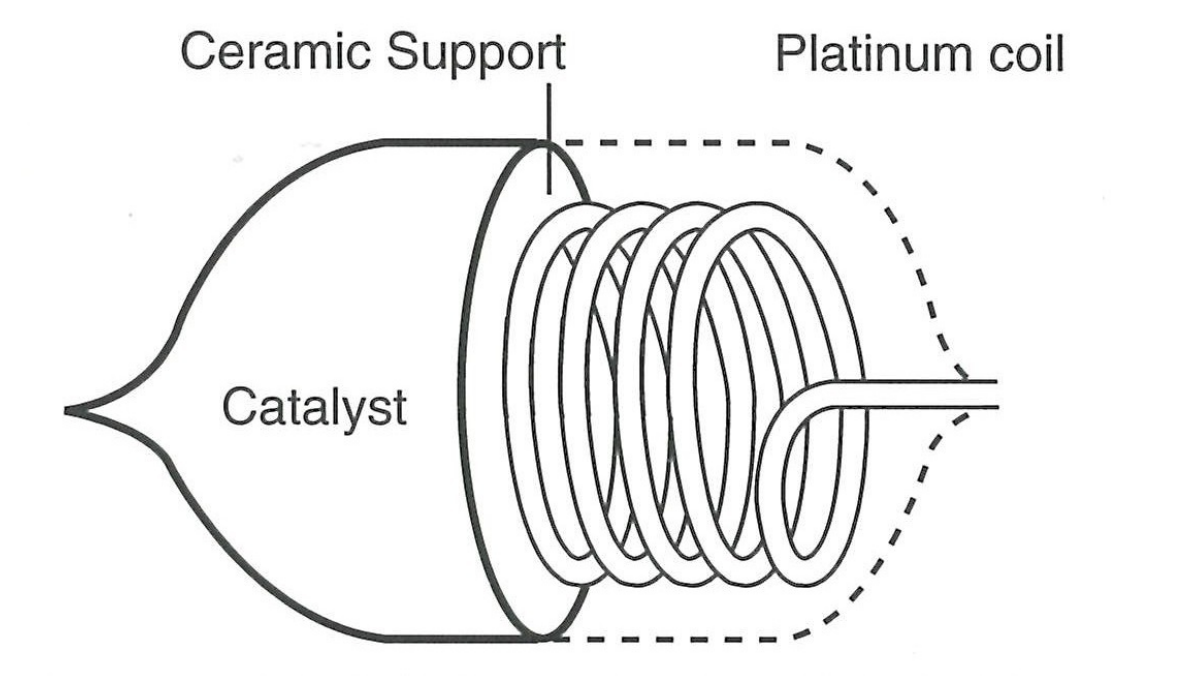
\includegraphics[scale=0.4, center]{catalytic.png}
    \caption[Structuur katalytische gassensor]{Interne structuur van een katalytische verbrandingsgassensor \autocite{gastec2016}}
    \label{fig:catalytic}
\end{figure}


\subsection{Elektrochemische gassensoren}
\label{subsec:elektrochemische}

Elektrochemische gassensoren gebruiken oxidatiereductiereacties om de gasconcentratie te meten. Wanneer een specifiek gas met het membraan (zie figuur~\ref{fig:elektrochemical}) in aanraking komt wordt het verdeeld in de elektrolyt. Deze elektrolyt kan van vast of vloeibaar materiaal zijn gemaakt. Wanneer de moleculen vervolgens in aanraking komen met de elektrode ondergaan deze een oxidatieve reactie. In deze reactie komen ionen en elektronen vrij. Zo kan er via een stroommetingssysteem worden bepaald hoeveel stroom er tussen de twee elektroden loopt (sensing- en counter elektrode in figuur~\ref{fig:elektrochemical}) \autocite{Stetter2008}.

Zo wordt de hoeveelheid gas vervolgens bepaald via de Coulomb-analyse. In deze analyse wordt de hoeveelheid gas bepaald op basis van de wet van Faraday \autocite{gvda2023}.

Deze soort gassensor kan een grote waaier aan gassen detecteren en heeft een hoge gevoeligheid \autocite{review2014}. Maar deze sensoren hebben een korte levensduur en hebben dus regelmatig nood aan onderhoud, waardoor ze niet geschikt zouden zijn als duurzame gassensor voor in een veestal.

\begin{figure}[h]
    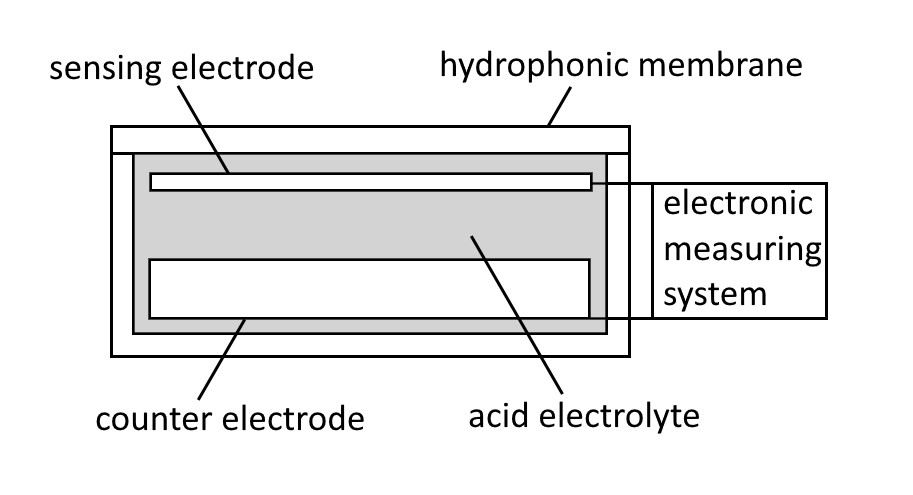
\includegraphics[scale=0.4, center]{elektrochemical.png}
    \caption[Structuur elektrochemisch gassensor]{Interne structuur van een elektrochemische gassensor \autocite{MajderLopatka2018}}
    \label{fig:elektrochemical}
\end{figure}



\subsection{Infrarood gassensoren}
\label{subsec:infrarood}

Een andere veelgebruikt gassensor is de infrarood gassensor (zie figuur~\ref{fig:infrarood}). Deze bestaat uit een lichtbron, een meetkamer en een detector. In deze lichtbron is ook een filter aanwezig. Deze filter is in staat om specifieke golflengtes van infrarood licht te selecteren.

Zo maakt de infrarood gassensor gebruik van het feit dat gasmoleculen in staat zijn om infrarode lichtstralen absorberen. Zo heeft ieder soort gas een eigen specifieke golflengte die wordt geabsorbeerd \autocite{li2010infrared}.

Wanneer de verzonden infraroodstralen de infraroodsensor verzwakt bereiken kan de gasconcentratie worden berekend. Dit gebeurt op basis van het verschil in de bereikte hoeveelheden infraroodstraling. Hoe meer gas er is, hoe minder infraroodstralen de sensor bereiken en omgekeerd \autocite{Senseair2018}. Wat betreft nauwkeurigheid en gevoeligheid is de infrarood gassensor superieur aan de andere soorten, en ook heeft deze soort sensor een langere levensuur dan de rest. Maar een infraroodsensor is wel een stuk duurder dan andere gassensoren. Ook kampt het met het probleem dat niet alle gassen infrarood licht kunnen absorberen, zoals bijvoorbeeld stikstof (N\textsubscript{2}) of waterstof (H\textsubscript{2}) \autocite{review2014}. Deze gassen kunnen dus niet worden gemeten.

\begin{figure}[h]
    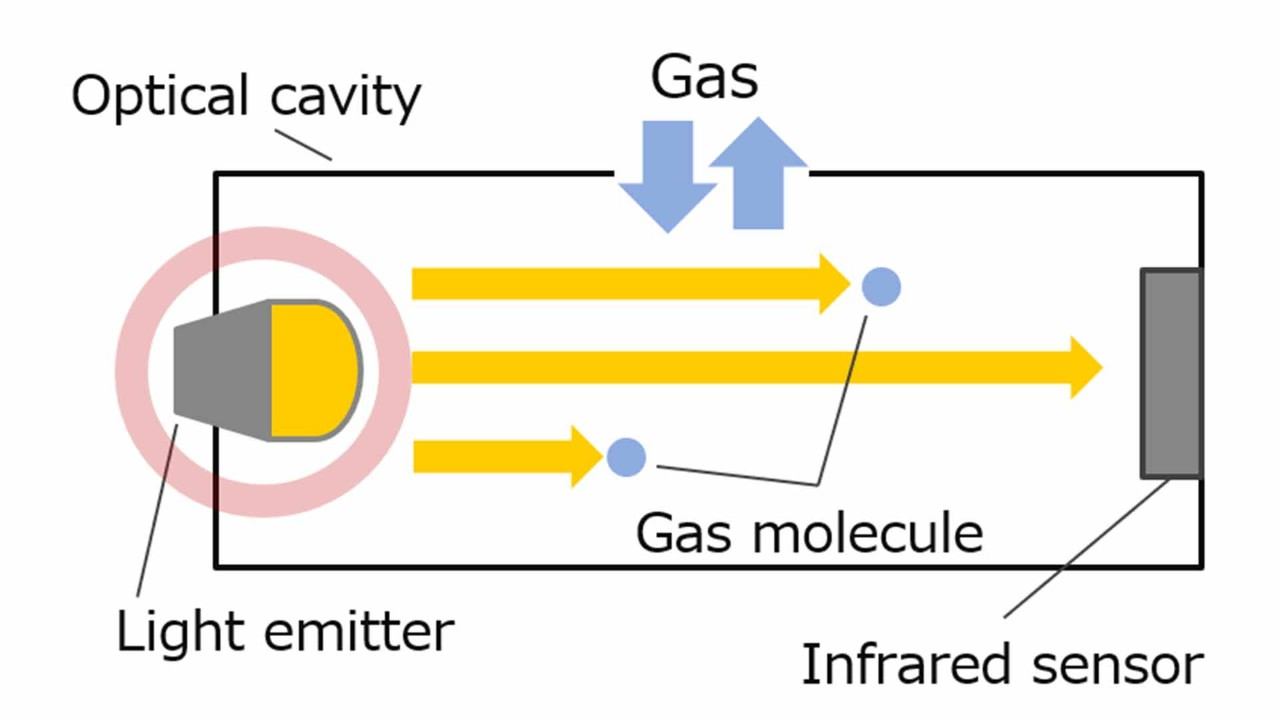
\includegraphics[scale=0.15, center]{infrarood.jpeg}
    \caption[Structuur infrarood gassensor]{Interne structuur van een infrarood gassensor \autocite{Senseair2018}}
    \label{fig:infrarood}
\end{figure}


\subsection{Halfgeleider gassensoren}
\label{subsec:MOS}

Volgens \textcite{wiki2022} is een halfgeleider een stof die op vlak van elektrische geleiding het midden houdt tussen goede geleiders en goede isolators. De halfgeleider die het meest wordt gebruikt bij gassensoren is tindioxide (SnO\textsubscript{2}) samen met een laag siliconen \autocite{Nikolic2020}. Wanneer het halfgeleidermateriaal in contact komt met een gasmolecule waarvoor het gevoelig is, treden er chemische reacties op aan het oppervlak van het materiaal. Deze reacties leiden tot veranderingen in de elektrische weerstand van het halfgeleidermateriaal. Het meetcircuit van de sensor detecteert deze verandering en zet deze om in een meetbare elektrische signaaluitgang \autocite{review2014}. Deze soort gassensoren hebben een hoge gevoeligheid, zijn goedkoop en kunnen en breed scala aan gassen detecteren. Het grootste nadeel van halfgeleider gassensoren is dat ze ook gevoelig zijn voor omgevingsfactoren zoals temperatuur en luchtvochtigheid, die de resultaten sterk kunnen beïnvloeden. Ook leiden ze aan kruisgevoeligheid, wat betekent dat ze kunnen ook reageren op andere gassen dan het doelgas, wat kan leiden tot vals-positieve resultaten.


\begin{figure}[h]
    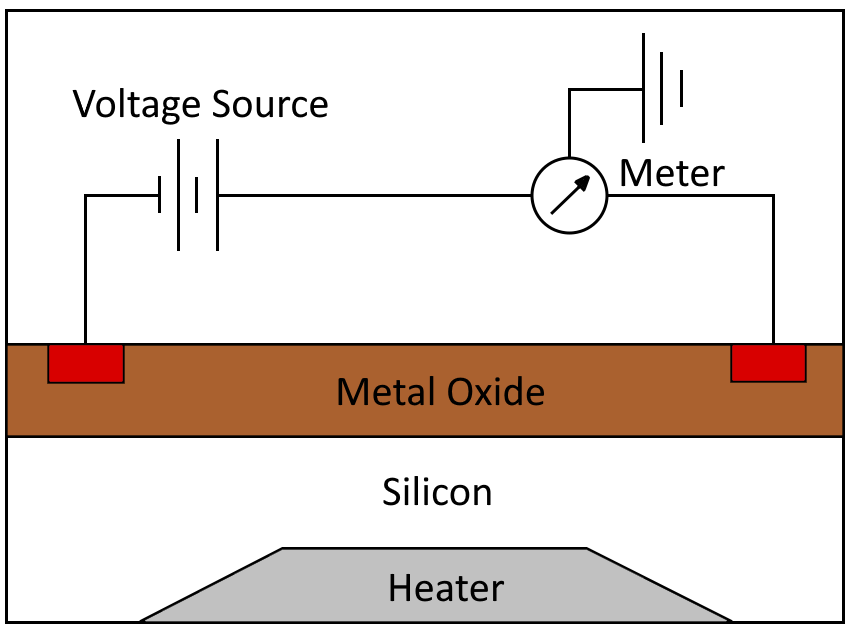
\includegraphics[scale=0.2, center]{halfgeleider.png}
    \caption[Structuur halfgeleider gassensor]{Interne structuur van een halfgeleider gassensor \autocite{review2014}}
    \label{fig:halfgeleider}
\end{figure}

\pagebreak

\section{Gebruikte hardware in de test set-up}
\label{sec:hardware}


\subsection{De MQ-gassensoren}%
\label{subsec:werking-MQ}

De MQ-gassensor is dus een gassensor van het type halfgeleider, ze kost twee tot vijf euro en kan gemakkelijk worden gebruikt via een microcontroller zoals Arduino. Het is belangrijk op te merken dat de MQ-gassensor meerdere gassen kan detecteren, maar deze niet afzonderlijk kan identificeren. De sensor geeft dus een enkele waarde terug.
De MQ-sensor heeft een voeding van 5V nodig \autocite{akp2023}, en omdat deze sensor via verwarming te werk gaat is deze beschermt met 2 lagen fijn roestvrij stalen gaas. Dit beschermende gaas zorgt ervoor dat het verwarmingselement in de sensor geen explosies veroorzaakt wanneer het in aanraking komt met een brandbaar gas.


\begin{figure}[h]
    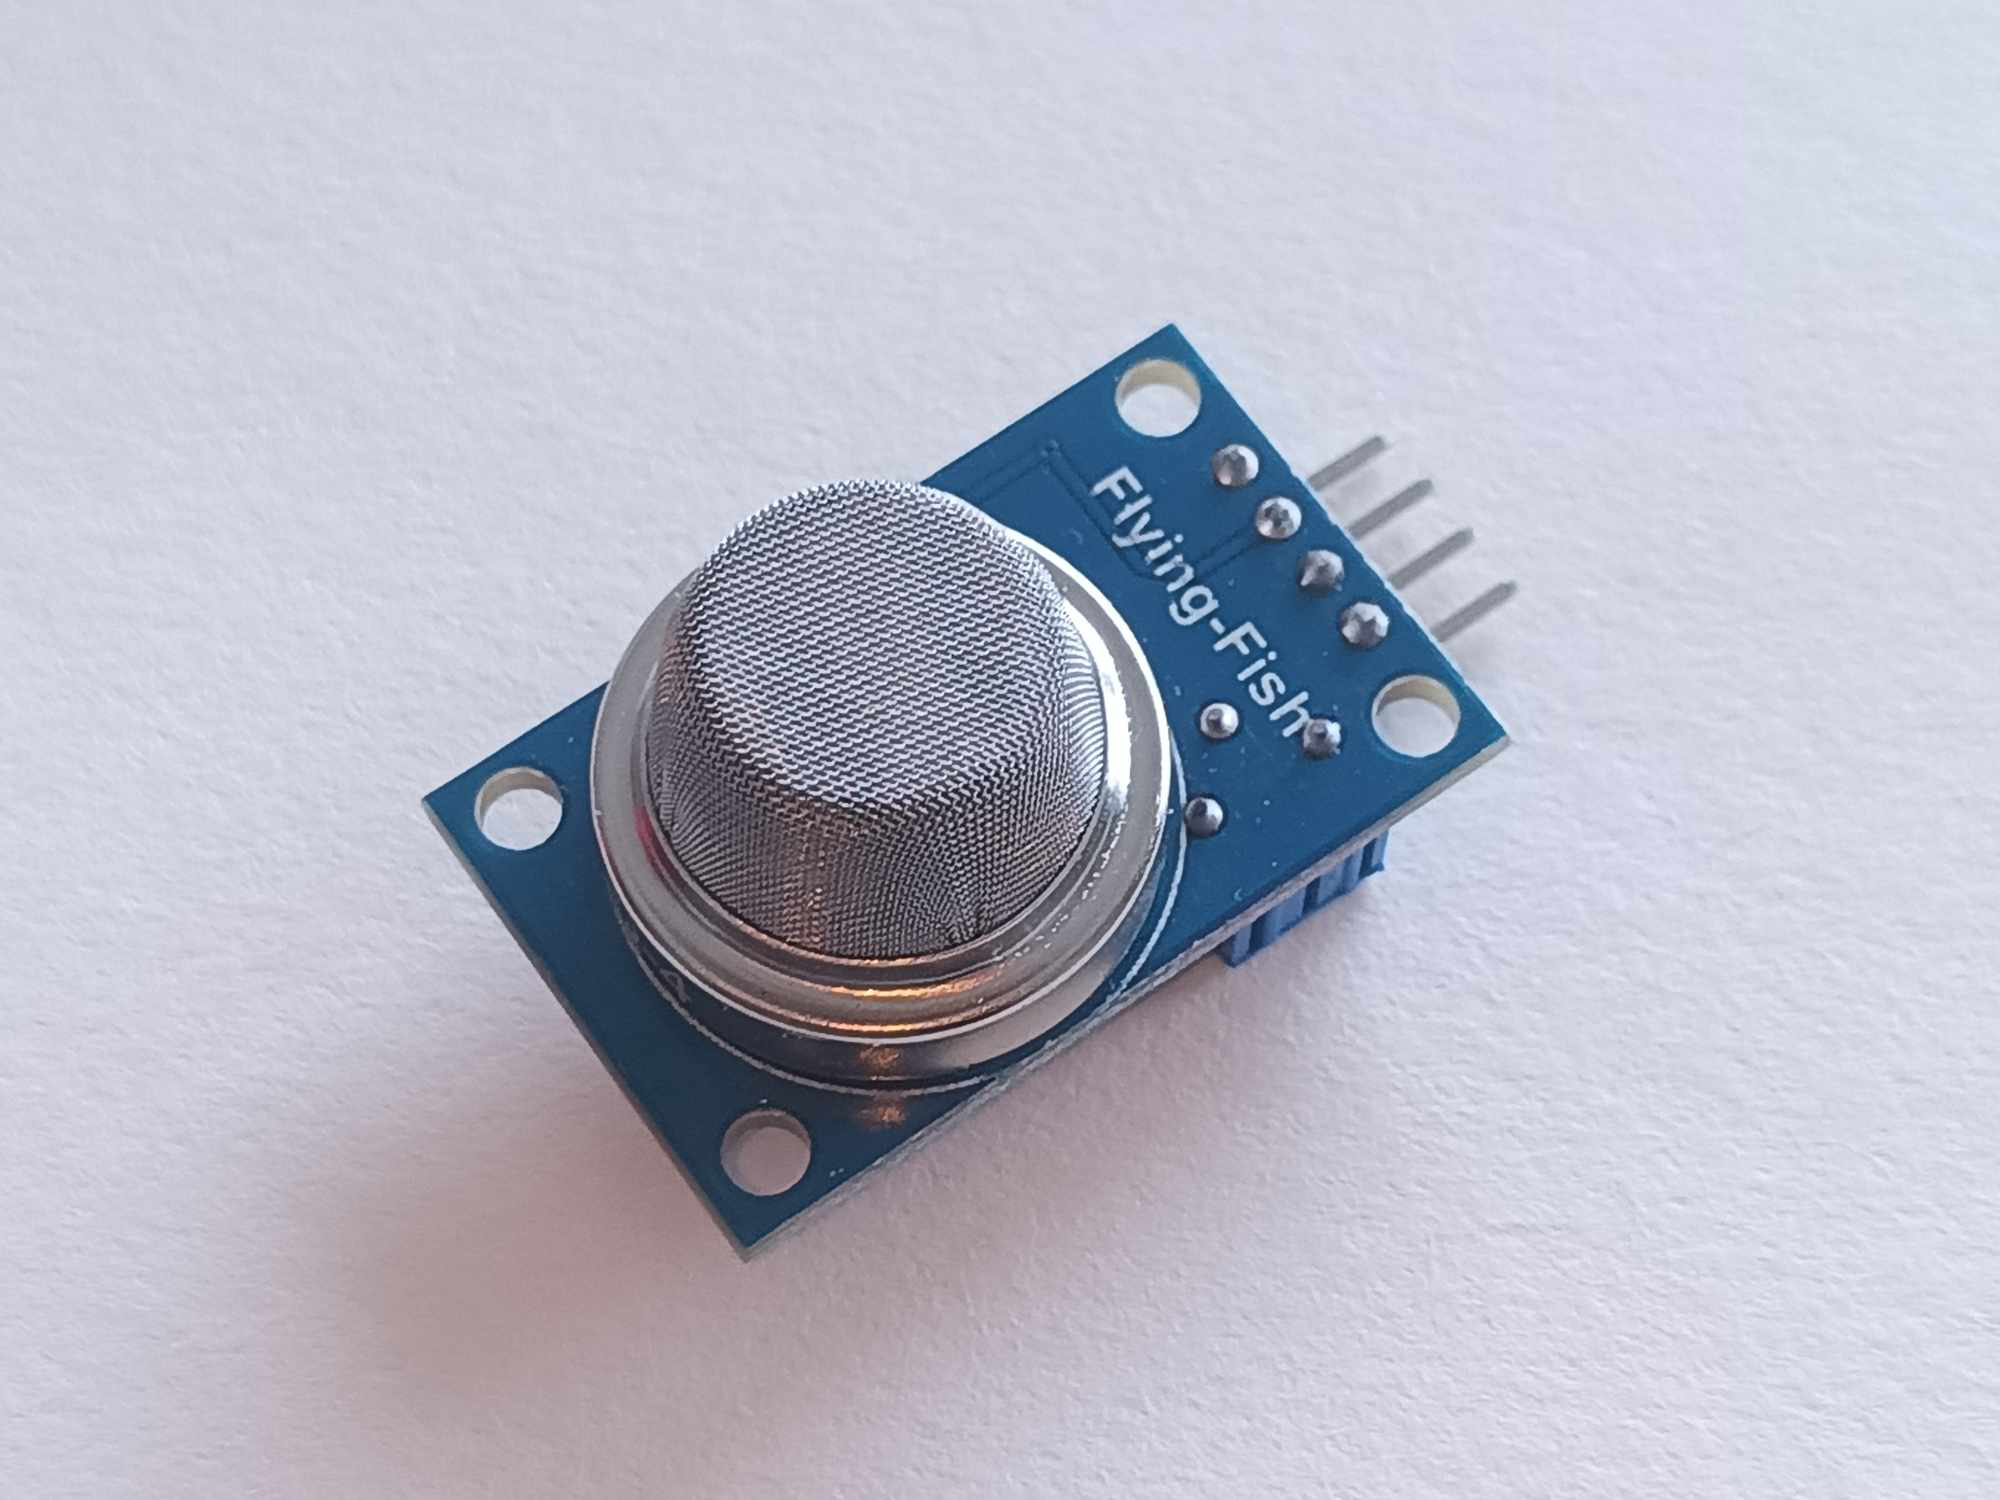
\includegraphics[scale=0.12, center]{mq.png}
    \caption[MQ-gassensor]{MQ-gassensor (links) en zijn interne structuur (rechts)}
    \label{fig:mq}
\end{figure}


De interne structuur van de sensor bestaat uit zes pinnen die verbonden zijn met een centraal sensorelement. De twee middelste pinnen zijn verantwoordelijk voor het verwarmen van het sensorelement, en de vier andere pinnen detecteren kleine variaties in de stroom die door het element gaat. Dit sensorelement bestaat uit keramiek op aluminiumoxidebasis (Al\textsubscript{2}O\textsubscript{3}), gecoat met een laag tindioxide (SnO\textsubscript{2}).


\begin{figure}[h]
    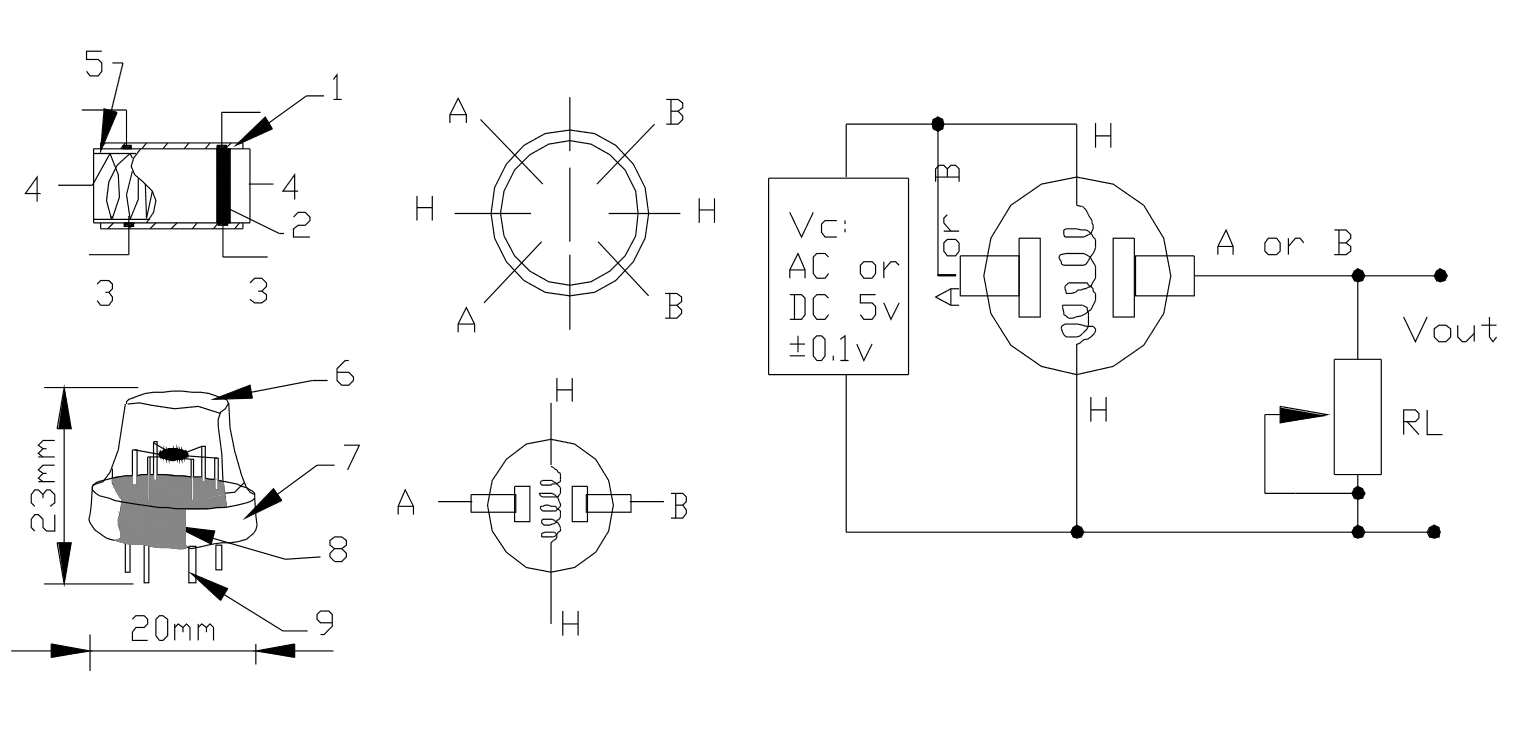
\includegraphics[scale=0.3, center]{mq_configuratie.png}
    \caption[Schema MQ-gassensor]{Schema van de structuur van een MQ-gassensor \autocite{mq4}}
    \label{fig:mq_configuratie}
\end{figure}

Wanneer deze laag SnO\textsubscript{2} wordt verwarmd blijven zuurstofmoleculen aan het oppervlak vast hangen door adsorptie. Hierdoor wordt een depletielaag gevormd, dit is een laag waar geen transport mogelijk is en dus een elektrisch isolerende laag wordt gevormd \autocite{dr2016}. Gevolglijk heeft de SnO\textsubscript{2} een hoge weerstand, waardoor de elektrische stroom wordt geblokkeerd.

Wanneer de omgeving echter andere gassen bevat kunnen deze de zuurstoflaag reduceren door middel van reductie. Als resultaat neemt de depletielaag af in dichtheid en komen er elektronen vrij in het SnO\textsubscript{2}-materiaal. Zo verminderd de weerstand en verhoogt de elektrische stroom.

Een belangrijk detail bij het gebruiken van de MQ-sensor is de voorverwarming. Doordat de sensor een lange tijd in opslag heeft gelegen verliest hij zijn nauwkeurigheid, daarom is het noodzakelijk om hem 24-48 uur te laten voorverwarmen. Hierna heeft de sensor bij iedere sessie slechts 5-10 minuten nodig om zich te stabiliseren \autocite{Sakayo2019}.

Er zijn veel verschillende soorten MQ-sensoren die elk gespecialiseerd zijn in verschillende gassen, volgens het onderzoek van \textcite{Khodadadi2001} kan de gevoeligheid voor methaan (CH\textsubscript{4}) vergroot worden door platina toe te voegen aan de SnO\textsubscript{2}. Ook kan door een toevoeging van K\textsubscript{2}O de gevoeligheid voor koolstofmonoxide (CO) worden vergroot. En op dezelfde manier kan Na\textsubscript{2}O ervoor zorgen dat de sensor minder gevoelig wordt voor CO\textsubscript{2}. Zo heeft iedere MQ-sensor kleine aanpassingen in het sensor element wat ze gevoelig maakt voor specifieke gassen.

De MQ-sensoren die gekozen zijn voor dit onderzoek zijn de MQ-4, MQ-7 en MQ-135. De MQ-4 sensor is gevoelig voor methaan (CH\textsubscript{4}) en LPG (Liquified Petroleum Gas). De MQ-7 biedt een specialisatie in koolstofmonoxide (CO) en waterstof (H\textsubscript{2}). Tenslotte is de MQ-135 een sensor die wordt gebruikt om de algemene luchtkwaliteit te meten, dit gebeurt vooral aan de hand van de gassen CO\textsubscript{2}, NH\textsubscript{4} en CO \autocite{RC2022}.

In dit onderzoek is er voor de MQ-4 en en MQ-135 sensor gewerkt met een module, dit betekent dat de sensor al op een vooraf gemaakte printplaat is bevestigd. Deze modules hebben geen zes maar vier pinnen: spanning, grond, digitale- en analoge uitgang. Het voordeel van deze modules is dat deze gemakkelijker te gebruiken zijn dan de naakte sensoren, maar het nadeel is dat de belastingsweerstand op deze modules gelijk is aan 1k$\Omega$. In de datasheets van deze sensoren (\autocite{mq135}, \autocite{mq4}) staat dat er voor optimale resultaten de aanbevolen belastingsweerstand 20k$\Omega$ is. 1 k$\Omega$ valt hier dus ver onder dus het is belangrijk hier rekening mee te houden als de ppm wordt berekend in de berekeningen (\ref{sec:hoe-luchtsamenstelling meten}).


\subsection{DHT22}%
\label{subsec:dht22}

Naast de MQ-sensoren zal ook een DHT22 sensor worden geïntegreerd in de test set-up. De DHT22 sensor meet temperatuur en luchtvochtigheid. Deze waarden kunnen van pas komen bij het optimaliseren van de resultaten van de MQ-sensoren, aangezien deze sensoren gevoelig zijn voor omgevingsfactoren zoals temperatuur en luchtvochtigheid.

In sectie~\ref{sec:temp-en-hum} zal worden berekend hoe de waarde van de MQ-sensor kan worden gecorrigeerd aan de hand van de temperatuur, de luchtvochtigheid en de info van de datasheet.

\begin{figure}[h]
    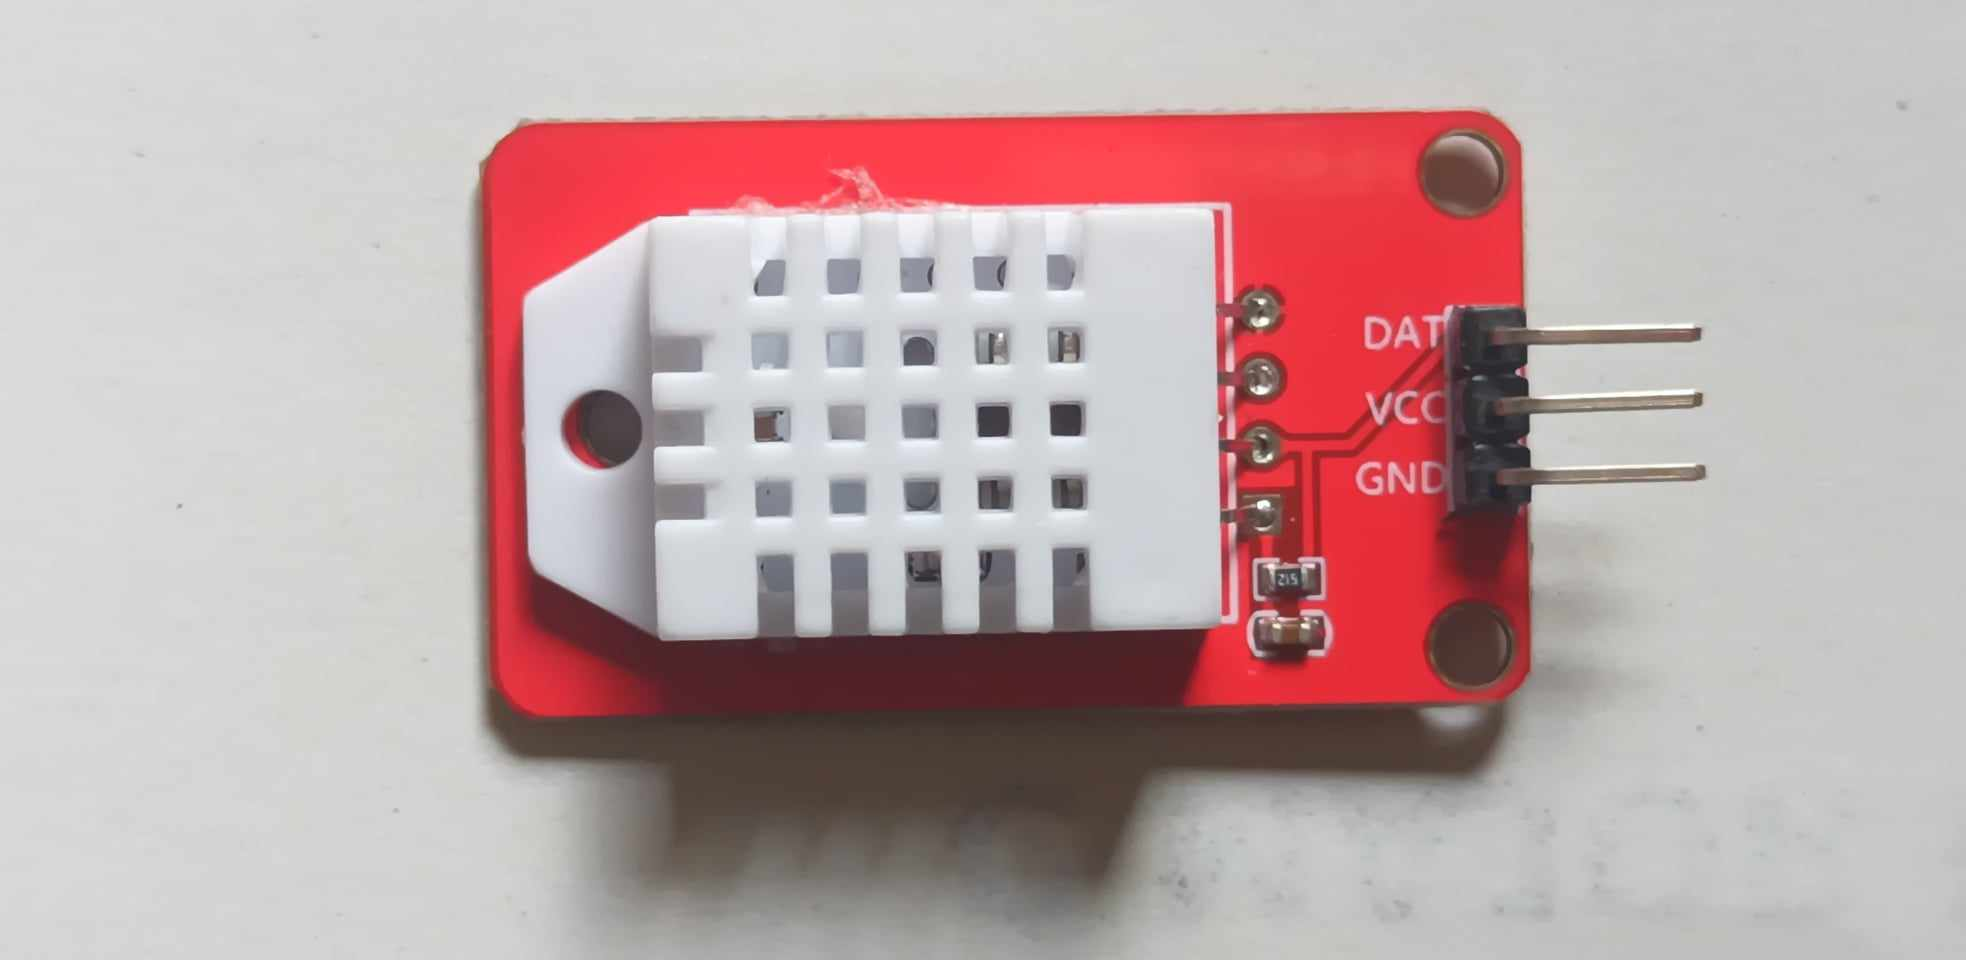
\includegraphics[scale=0.1, center]{dht22.jpg}
    \caption[DHT22 sensor]{De DHT22 sensor}
    \label{fig:dht22}
\end{figure}


\subsection{Arduino Mega 2560 Microcontroller}%
\label{subsec:arduino}

Voor dit onderzoek werd de Arduino Mega 2560 gekozen als microcontroller. De Arduino Mega 2560 is iets groter en krachtiger in vergelijking met de basis Arduino Uno voor een iets duurdere prijs. De Arduino Mega biedt een flashgeheugen van 256 KB, 54 I/O pins, 16 analoge input pins, een EEPROM (Electrically erasable programmable read-only memory) van 4kB en een SRAM (Static random-access memory) van 8 kB \autocite{Arduino}.

\begin{figure}[h]
    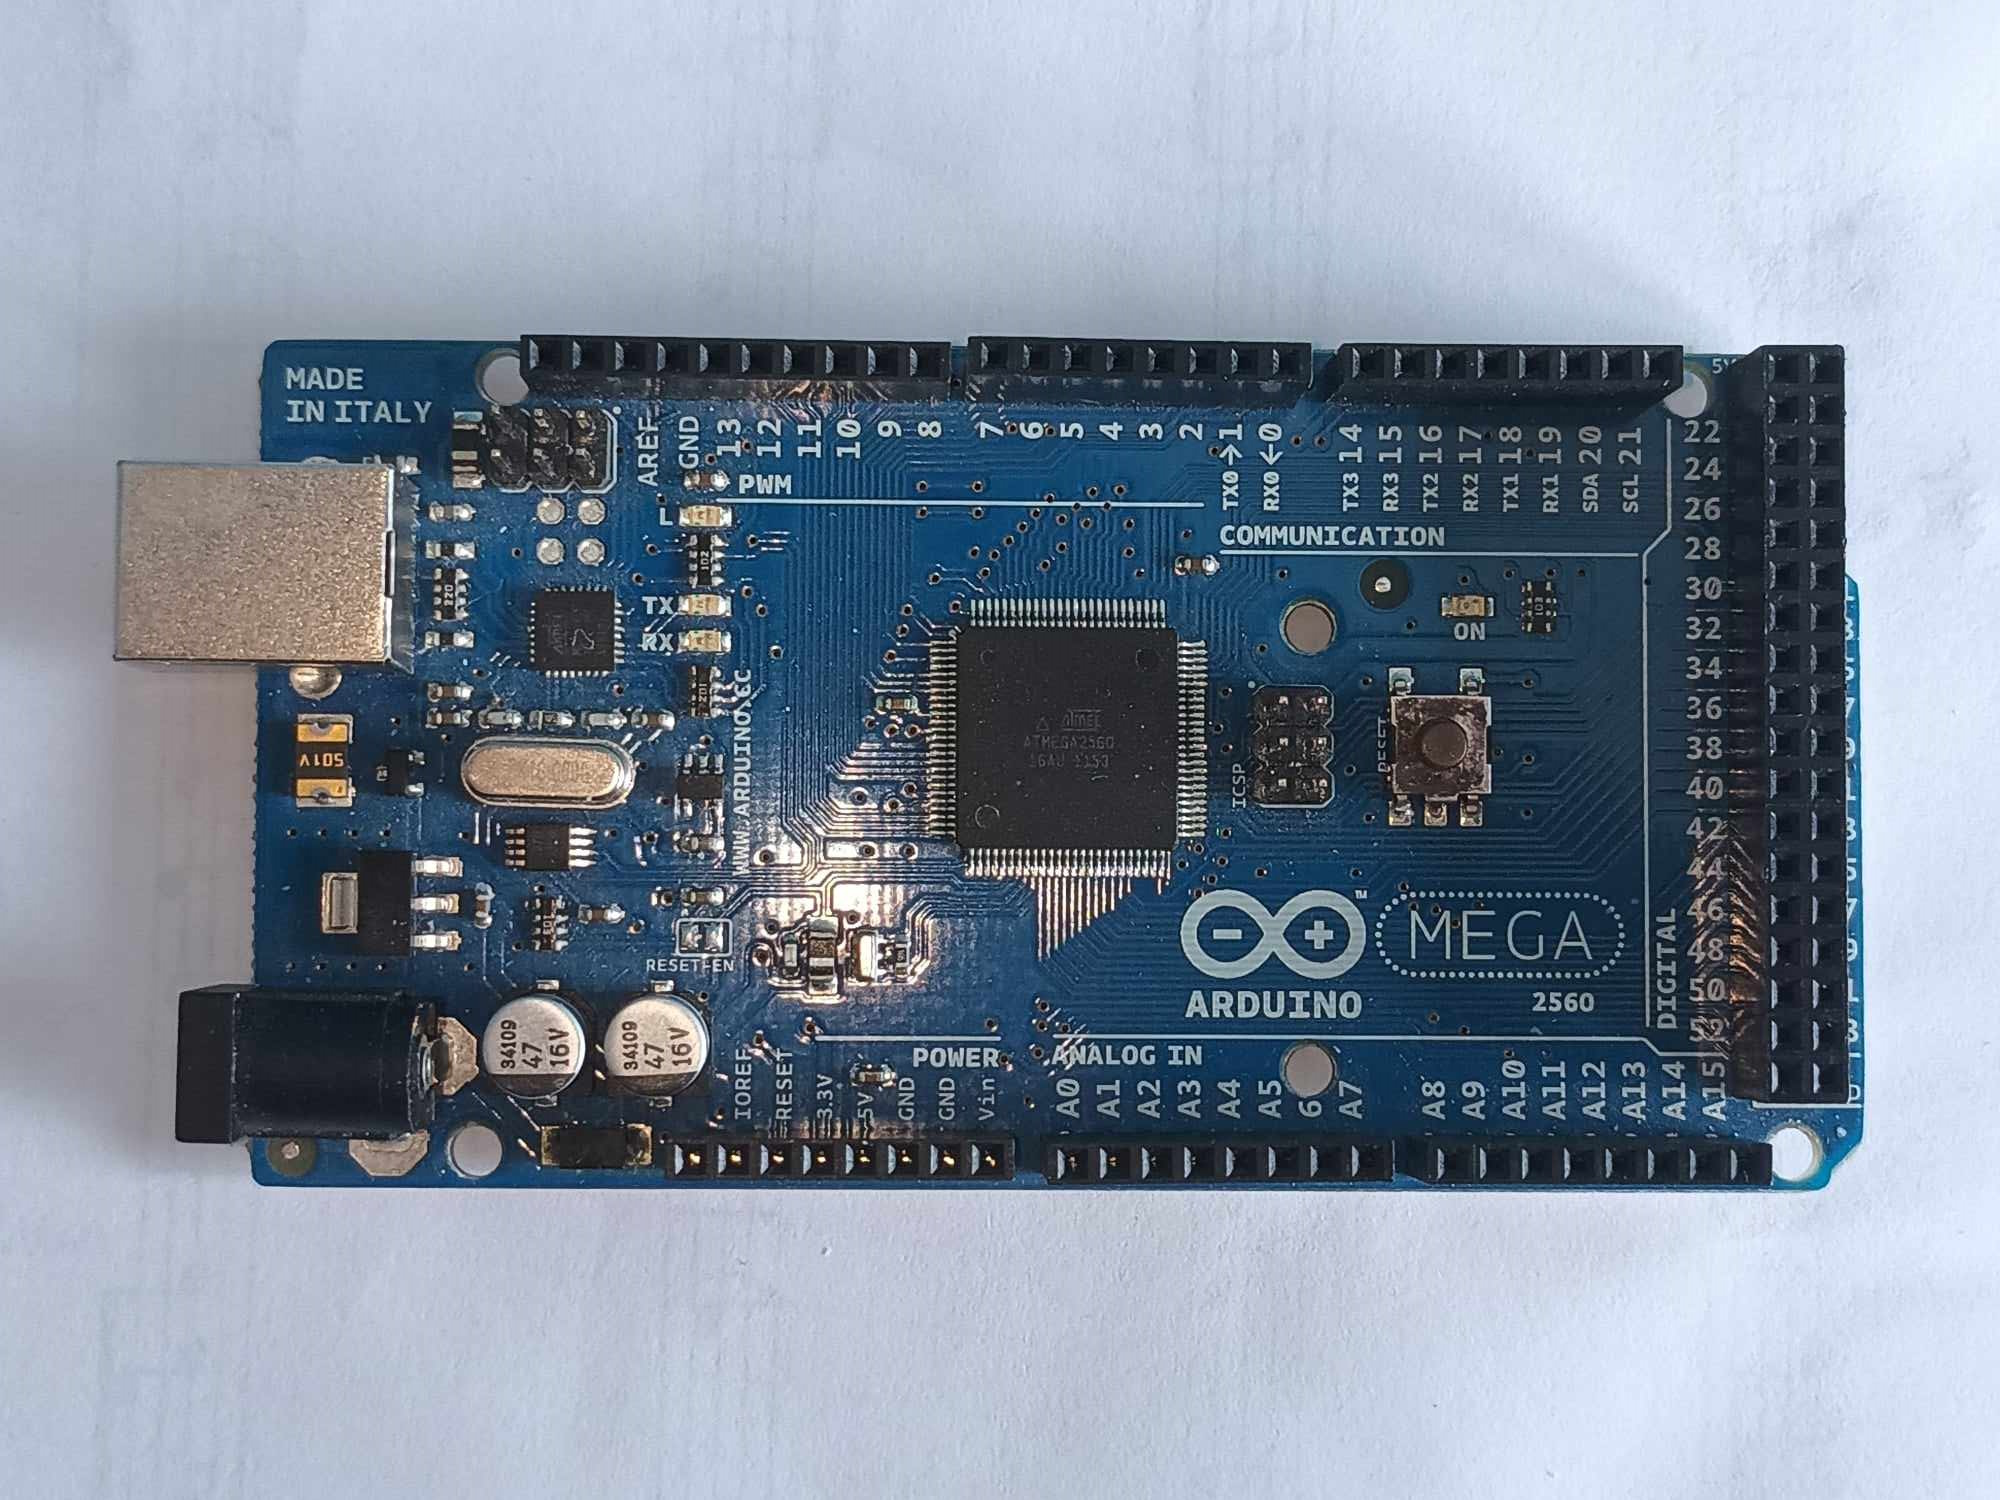
\includegraphics[scale=0.1, center]{arduino.jpg}
    \caption[Arduino Mega]{De Arduino Mega 2560}
    \label{fig:arduino}
\end{figure}


Via de Arduino IDE kan de microcontroller gemakkelijk worden geprogrammeerd om de sensoren uit te lezen en deze door te sturen naar de WiFi module.

\subsection{ESP8266-01s WiFi Module}%
\label{subsec:esp01}

De ESP8266-01s, of in het kort de ESP01, is een kleine en goedkope module die data kan versturen over een WiFi-netwerk, mits ze is aangesloten op dat netwerk. De ESP01 werkt via AT commando's, ook wel gekend als de Hayes Command Set \autocite{Bales2023}. Deze commando's worden vooral gebruikt om een ​​modem te configureren en de netwerkverbinding tot stand te brengen, maar ze zijn ook in staat data te versturen via een TCP of UDP verbinding. Zo kunnen de waarden die terug worden gegeven door de sensoren worden verzonden naar een databank en het Thingspeak platform.
Het AT-commando bestaat algemeen uit drie delen: de prefix, body en terminator. De prefix bestaat steeds uit ``AT''. De body bestaat uit de werkelijke opdracht, samen met parameters en andere gegevens. Ten slotte is er de terminator, deze is doorgaans een newline (\textbackslash r\textbackslash n) \autocite{Teltonika}.

\begin{figure}[h]
    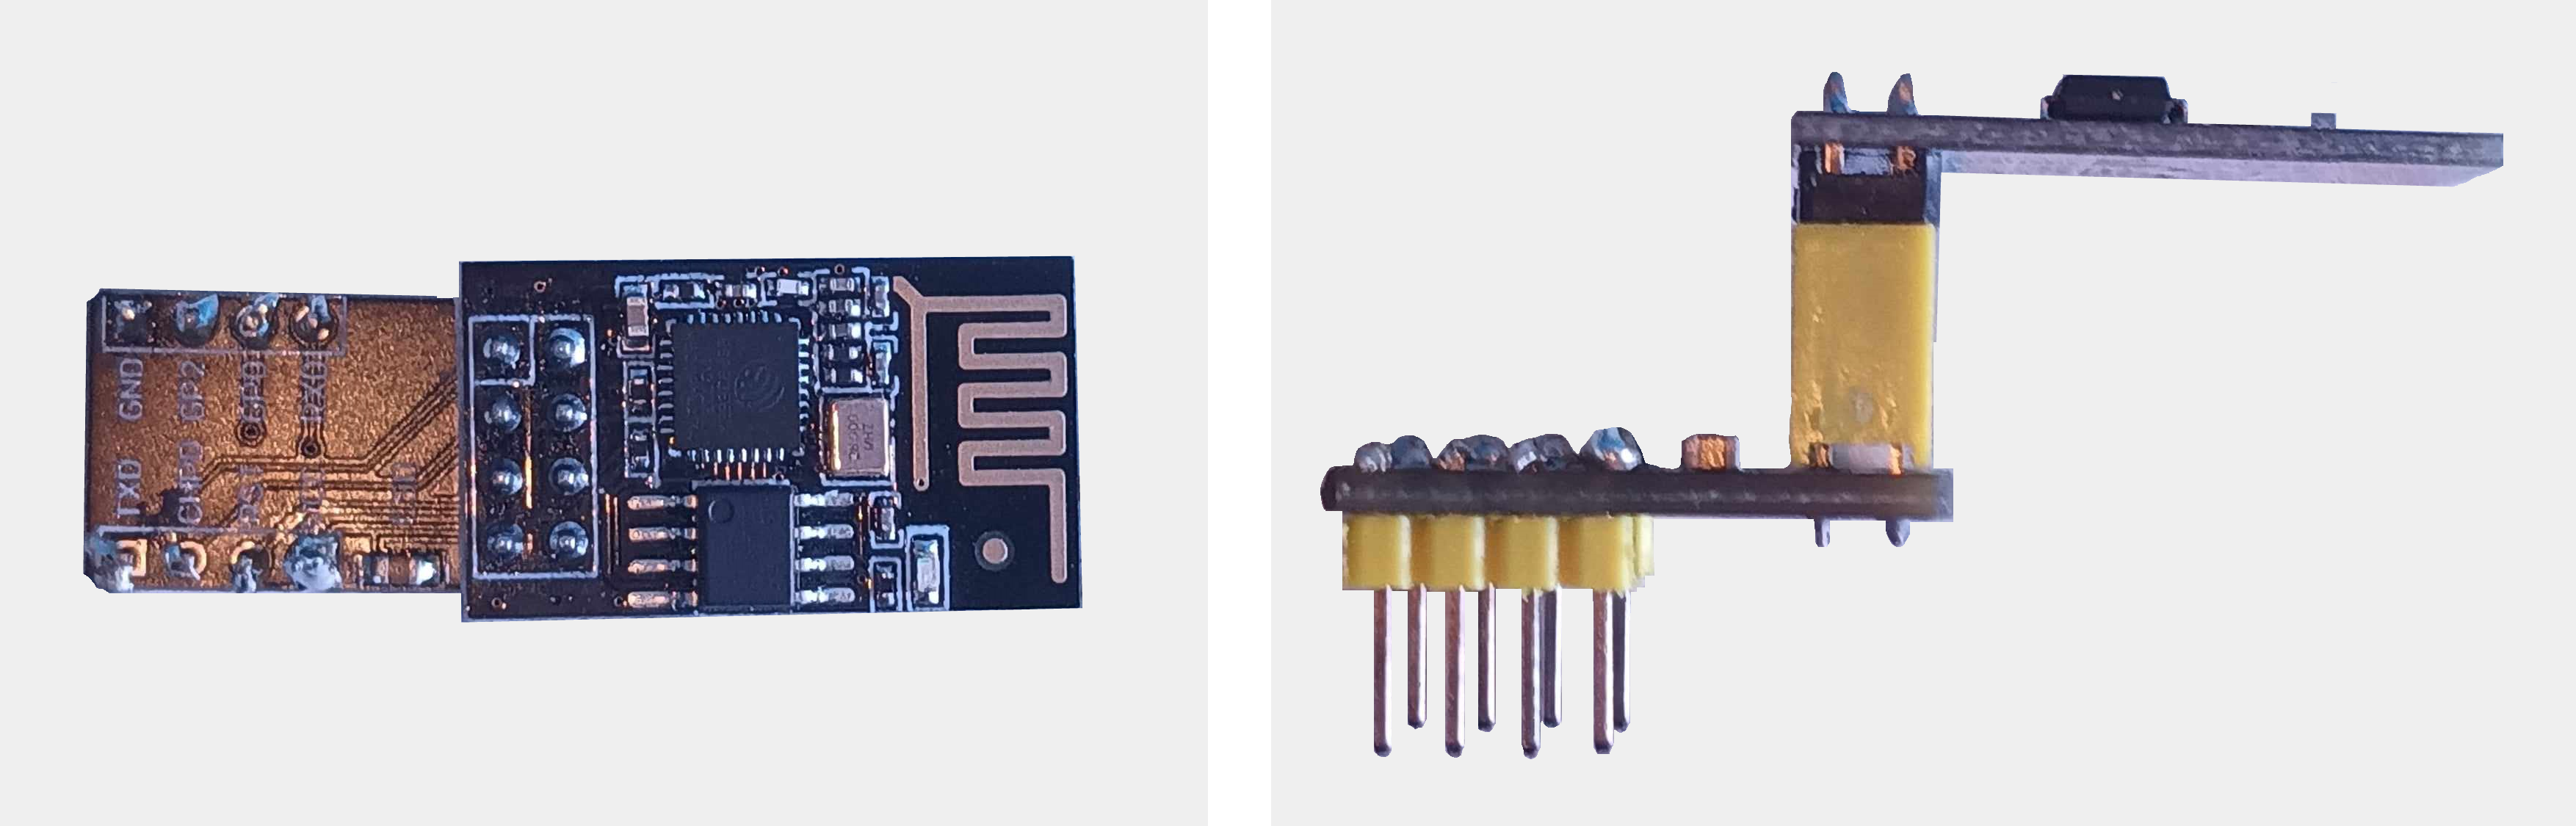
\includegraphics[scale=0.18, center]{esp.png}
    \caption[ESP01 WiFi module]{De ESP01 WiFi module met een breadboard-adapter}
    \label{fig:esp}
\end{figure}



\section{Hoe kan de luchtsamenstelling worden gemeten door MQ-sensoren?}%
\label{sec:hoe-luchtsamenstelling meten}

Een MQ-sensor geeft dus maar 1 analoge waarde terug, maar op basis van deze waarde kan een berekende schatting worden gemaakt naar de luchtsamenstelling. In de officiële datasheets van de MQ-4, -7 en -135 staan gevoeligheidscurves voor de soorten gas waar die sensor het meest gevoelig voor is (\autocite{mq4}, \autocite{mq7}, \autocite{mq135}). Zo zie je in figuur~\ref{fig:MQ135_grafiek} een voorbeeld van de gevoeligheidscurve van de MQ-135 sensor.

\begin{figure}[h]
    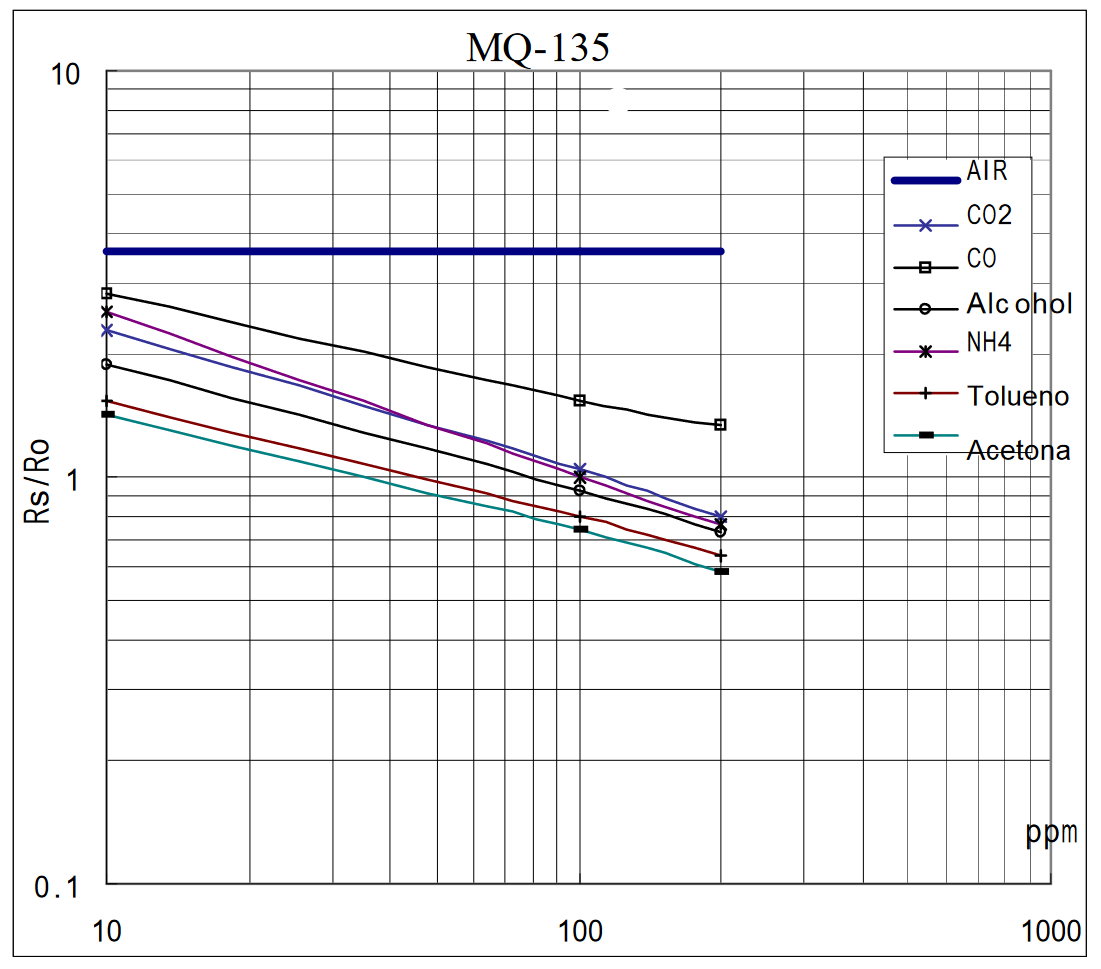
\includegraphics[scale=0.5, center]{MQ135_grafiek.png}
    \caption[Gevoeligheidscurve MQ-135]{Gevoeligheidscurve van de MQ-135 sensor \autocite{mq135}}
    \label{fig:MQ135_grafiek}
\end{figure}

\pagebreak

Via deze curves kan per type gas de PPM worden berekend, maar daarvoor moet Rs/R\textsubscript{0} zijn gekend. De volgende berekeningen tonen hoe Rs en R0 kunnen worden berekend, waarmee vervolgens een analoge waarde kan worden omgezet naar PPM.

Het omzetten van de analoge waarden (0-1023) die Arduino teruggeeft naar spanningswaarden gaat als volgt:
\begin{equation}
    Vout = \frac{analoge\_waarde * Vcc}{max\_analoge\_waarde}
\end{equation}
Met Vcc = voedingsspanning in het circuit (= 5V) en max\_analoge\_waarde = 1023.

Daarna moet Rs worden gevonden, we beginnen met de wet van Ohm (met U = spanning in V, I = stroomsterkte in A en R = weerstand in $\Omega$):
\begin{equation}
    U = I * R
\end{equation}
\begin{equation}
    I = \frac{U}{R}
\end{equation}
\begin{equation}
    I = \frac{Vcc}{Rs+Rl}
\end{equation}
Met Rl = belastingsweerstand van het circuit en Rs = weerstand van de sensor

Terug naar Ohm:
\begin{equation}
    U = I * R
\end{equation}
\begin{equation}
    VRL = \frac{Vcc}{Rs + Rl} * Rl
\end{equation}
Met VRL = voltage reference low \textbf{(= Vout)}
\begin{equation}
    Rs = \frac{Vcc * Rl}{VRL} - Rl
\end{equation}
Nu de formule voor Rs te berekenen gekend is, moeten we kijken naar R0. R0 is de weerstand van de sensor in schone lucht. Op de gevoeligheidscurve (\ref{fig:MQ135_grafiek}) is te zien hoe Rs/R\textsubscript{0} een constante is voor schone lucht. Via software zoals WebPlotDigitizer \autocite{Rohatgi2024} kan de waarde van deze constante worden opgehaald. Voor de MQ-135 is deze waarde 3,6.

Dus:
\begin{equation}
    \frac{Rs}{R_0}(voor\ schone\ lucht) = 3,6
\end{equation}
\begin{equation}
    R_0 = \frac{Rs}{3,6}
\end{equation}
Om de sensor te kalibreren moet dus de R\textsubscript{0} waarde worden berekend. Het is dus zeer belangrijk dat de sensor 24-48 heeft voorverwarmd en dat de kalibratie in schone lucht gebeurt, anders kan de R\textsubscript{0} waarde afwijken en zullen de lezingen incorrect zijn.

Om de ppm waarde te berekenen kijken we opnieuw naar de gevoeligheidscurves (\ref{fig:MQ135_grafiek}). Deze curves lijken lineair te dalen, maar deze grafiek is dubbellogaritmisch. Volgens \textcite{loglog2024} is de vergelijking voor een lineaire curve in een dubbellogaritmische weergave de volgende:
\begin{equation}
    F(x) = x^{m} * 10^{b}
\end{equation}
Met m = gradiënt (de helling) en b = het snijpunt met de Y-as.

Volgens de MQ-135 grafiek is dit dan:
\begin{equation}
    \label{eq:grafiek}
    \frac{Rs}{R_0} = ppm^{m} * 10^{b}
\end{equation}
\begin{equation}
    \log_{10} (\frac{Rs}{R_0}) = m * \log_{10} (ppm) + b
\end{equation}
Om de ppm van een specifiek gas te berekenen hebben we $m$ en $b$ nodig. Hiervoor nemen we 2 punten op de curve van het gewenste gas waarvoor de ppm moet worden berekend (\ref{fig:MQ135_grafiek}), dit kan opnieuw worden gedaan met WebPlotDigitizer \autocite{Rohatgi2024}. Deze punten zullen we $x1,\ x2,\ y1\ en\ y2$ noemen:
\begin{eqnarray}
    \begin{cases}
        \log_{10} (y1) = m * \log_{10} (x1) + b\\
        \log_{10} (y2) = m * \log_{10} (x2) + b\\
    \end{cases}
\end{eqnarray}
\begin{eqnarray}
    \begin{cases}
        m = \frac{log_{10} (y2) - log_{10} (y1)}{log_{10} (x2) - log_{10} (x1)} \\
        b = log_{10} (y1) - m * log_{10} (x1)\\
    \end{cases}
\end{eqnarray}
Nu dat $m$ en $b$ zijn gekend kan de ppm worden berekend via vergelijking~\ref{eq:grafiek}:
\begin{equation}
    ppm = \Big(\frac{Rs}{R_0 * 10^{b}}\Big)^{\frac{1}{m}}
\end{equation}

De volgende bronnen werden geraadpleegd bij het berekenen van deze waarden: \autocite{ohm2024}, \autocite{Cornelius2022}, \autocite{KumarSai2019}, \autocite{Dorcea2018}, \autocite{jaycon2023}, \autocite{Kalra2016}, \autocite{RapidTables}, \autocite{Ibrahim2022}, \autocite{Gironi2014} en \autocite{Gironi2017}.



\section{Hoe gaat een sensor met een warmte-koelcyclus te werk?}%
\label{sec:warmte-koelcyclus}


Volgens de officiële datasheet van de MQ-7 sensor is het werkingsprincipe voor deze sensor anders dan de MQ-4 en -135 sensoren. Voor optimale resultaten moet er namelijk gebruik worden gemaakt van een warmte-koelcyclus. In deze cyclus wordt doorheen twee fases gegaan, een fase van lage verwarming en een fase van hoge verwarming. Tijdens de lage temperatuurfase wordt gedurende 90 seconden 1,4V naar de sensor verzonden. In deze fase wordt gas geabsorbeerd op de plaat, op het einde kan de waarde worden afgelezen. Tijdens de hoge temperatuurfase wordt gedurende 60 seconden 5V naar de sensor verzonden. In deze fase verdampen geabsorbeerde gassen van de sensorplaat, waardoor deze wordt gereinigd voor de volgende meting \autocite{Kobbekaduwa2021}. Een duidelijk voorbeeld hiervan is te zien in de figuur (\ref{fig:heat_cool_datasheet}) van de datasheet

\begin{figure}[h!]
    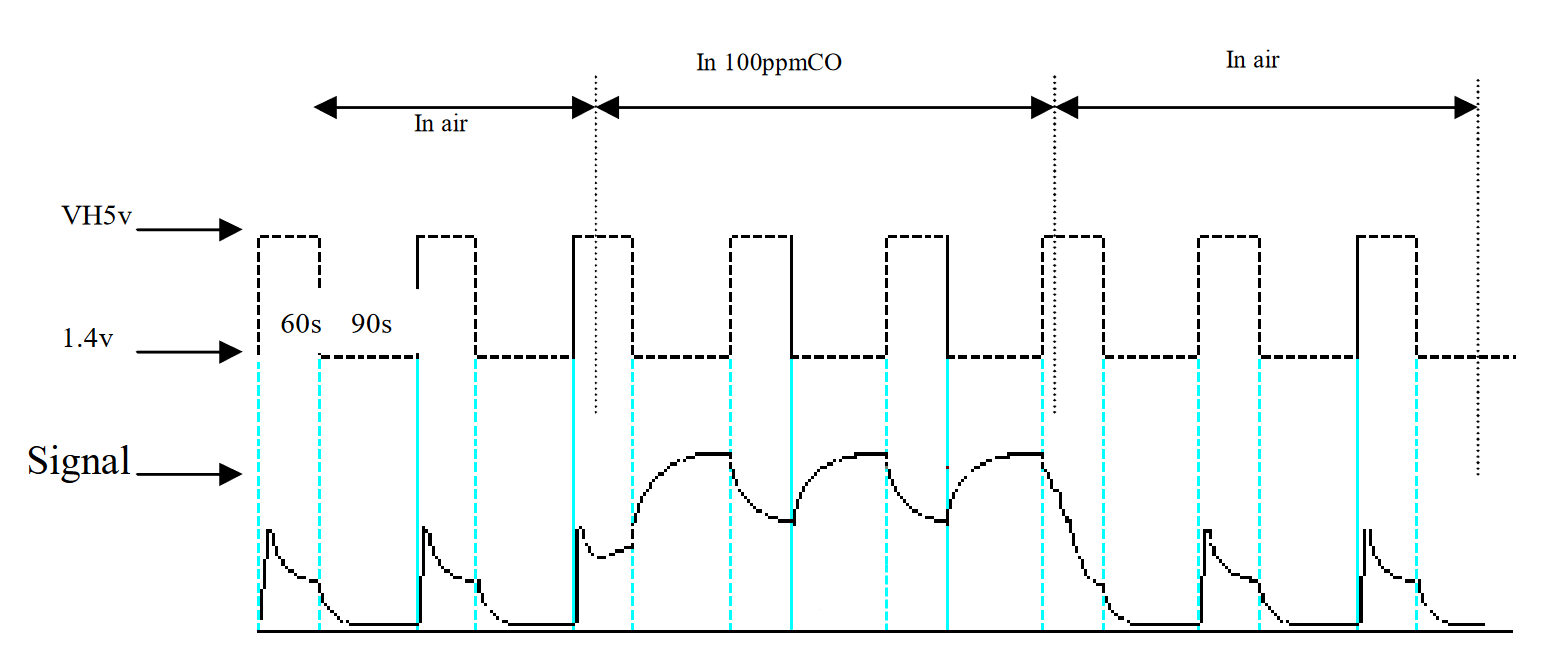
\includegraphics[scale=0.3, center]{heat_cool_datasheet.png}
    \caption[Warmte-koelcyclus MQ-7]{Een voorbeeld van de warmte-koelcyclus in de datasheet van de MQ-7 \autocite{mq7}}
    \label{fig:heat_cool_datasheet}
\end{figure}

In de studie van \textcite{Kobbekaduwa2021} is te zien hoe deze warmte-koelcyclus kan worden geïmplementeerd. De benodigde materialen (naast de MQ-7 en Arduino) zijn twee weerstanden van 10$k\Omega$ en een MOSFET transistor van het type IRF2807.


\section{Hoe kunnen de temperatuur en luchtvochtigheid tot nauwkeurigere resultaten leiden?}
\label{sec:temp-en-hum}

Zoals besproken in~\ref{subsec:MOS} zijn halfgeleider gassensoren gevoelig voor omgevingsfactoren zoals temperatuur en luchtvochtigheid. Een sensor zoals de DHT22 \autocite{Liu} kan deze omgevingsfactoren meten en kan zo de resultaten van de MQ-sensoren optimaliseren.

Volgens \textcite{Kalra2016} en \textcite{Cornelius2023} kan $Rs$ worden gecorrigeerd om zo een correctere ppm te verkrijgen. In de datasheets (\autocite{mq4}, \autocite{mq7}, \autocite{mq135}) van de MQ-sensoren staan naast gevoeligheidscurves grafieken die de invloed van temperatuur en vochtigheid weergeven. Zo zie je bijvoorbeeld in figuur~\ref{fig:MQ135_grafiek2} de afhankelijkheidsgrafiek van de MQ-135 datasheet.

\begin{figure}[h]
    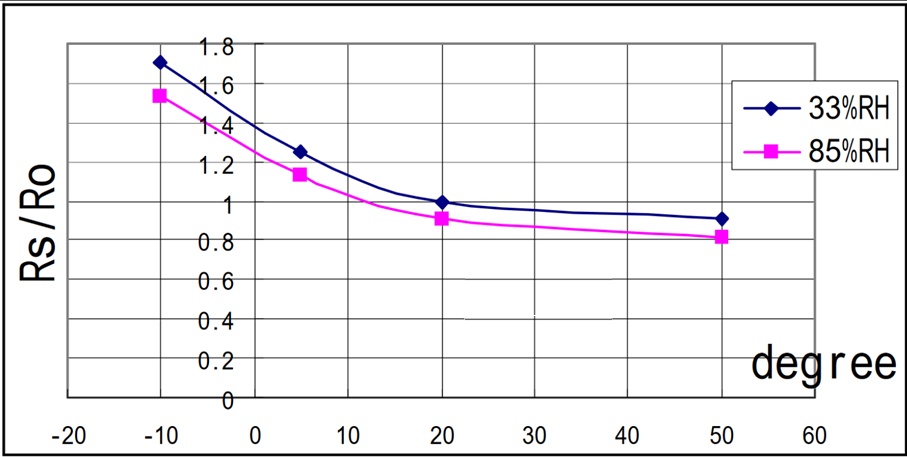
\includegraphics[scale=0.55, center]{MQ135_grafiek2.png}
    \caption[Afhankelijkheid temperatuur en luchtvochtigheid op MQ-135]{Afhankelijkheidsgrafiek van temperatuur en luchtvochtigheid op de resultaten van de MQ-135 \autocite{mq135}}
    \label{fig:MQ135_grafiek2}
\end{figure}

In de blog van software-ingenieur \textcite{Gironi20172} en in de studie van \textcite{Sukhdev2022} wordt vastgesteld dat via lineaire interpolatie de juiste correctiefactor kan worden berekent.

Aan de hand van de volgende stappen wordt duidelijk gemaakt hoe de correctiefactor kan worden berekend:

We beginnen met de afhankelijkheidsgrafiek van de datasheet (\ref{fig:MQ135_grafiek2}). Hier is te zien hoe Rs/R\textsubscript{0} kleiner wordt naarmate de temperatuur en vochtigheidsgraad stijgen. Via WebPlotDigitizer kunnen opnieuw de waarden uit deze grafieken gehaald worden \autocite{Rohatgi2024}. Hierna kan er via de \verb|polyfit| functie van Python package \verb|numpy| curve fitting worden gedaan op deze datapunten, zoals in de volgende listing:
\begin{lstlisting}[language=Python, caption={Curve fitting in Python}]
import pandas as pd
import numpy as np

mq135_humidity_33 = {'x': [ datapunten x ],
                    'y': [ datapunten y ]}
mq135_humidity_33_df = pd.DataFrame(mq135_humidity_33)

mq135_humidity_33_fit = np.polyfit(mq135_humidity_33_df['x'], mq135_humidity_33_df['y'], 2) #functie van de 2de graad

\end{lstlisting}

Als dit voor alle grafieken wordt gedaan wordt het resultaat in figuur~\ref{fig:curve_fitting_NOG_NIET} verkregen.

\begin{figure}[h]
    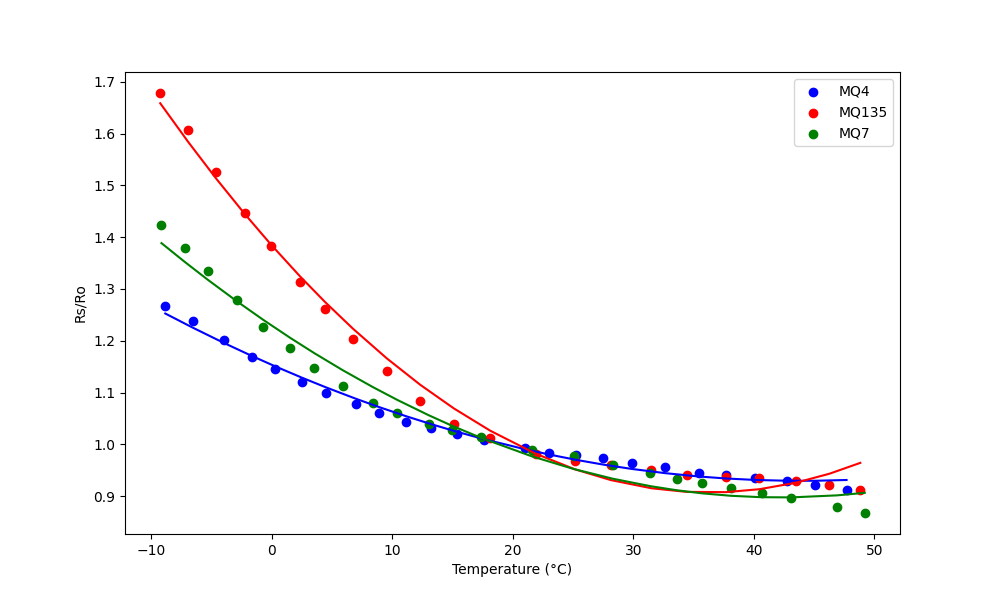
\includegraphics[scale=0.43, center]{curve_fitting_NOG_NIET.png}
    \caption[Niet optimale curve-fit op de datapunten]{Niet optimale curve-fit op de datapunten}
    \label{fig:curve_fitting_NOG_NIET}
\end{figure}

In deze grafiek is te zien hoe de curve fitting vanaf 20°C niet meer correct is, daarom zal de curve fitting worden opgesplitst. Voor de temperaturen onder 20°C zal een functie van de 2\textsubscript{de} graad worden toegepast, voor alle temperaturen hierboven zal gebruik worden gemaakt van een lineaire functie. Het resultaat is te zien in figuur~\ref{fig:curve_fitting_GOED}.

\begin{figure}[!h]
    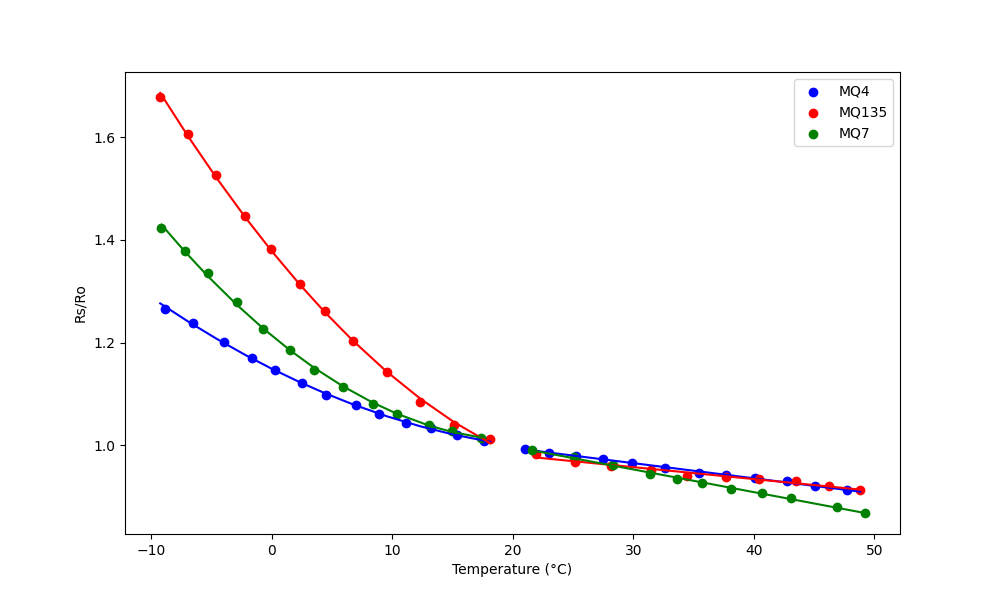
\includegraphics[scale=0.43, center]{curve_fitting_GOED.png}
    \caption[Optimale curve-fit op de datapunten]{Optimale curve-fit op de datapunten}
    \label{fig:curve_fitting_GOED}
\end{figure}

Zo zijn de functies voor de MQ-135 (\ref{fig:MQ135_grafiek2}) de volgende:

\(MQ135\_humidity\_33\_under\_20\ =\ 0.00046 * x^2 - 0.02907 * x + 1.37849\) \\
\(MQ135\_humidity\_85\_under\_20\ =\ 0.00041 * x^2 - 0.02534 * x + 1.24596\) \\
\(MQ135\_humidity\_33\_over\_20\ =\ -0.00233 * x + 1.02679\) \\
\(MQ135\_humidity\_85\_over\_20\ =\ -0.00273 * x + 0.95286\)

Nu de vergelijkingen voor alle grafieken gekend zijn kan de correctiefactor worden berekend. In het volgende voorbeeld wordt aangetoond hoe dit kan: stel dat we met de MQ-135 sensor een meting hebben gedaan waarbij de $temperatuur$ gelijk is aan $23$°C en de $vochtigheidsgraad$ gelijk is aan $55\%$. Aangezien de temperatuur boven de 20°C ligt zullen de lineaire vergelijkingen worden gebruikt.
Eerst zal Rs/R\textsubscript{0} worden berekend voor $temperatuur = 23$°C:

\begin{equation}
    F\_33(t) = -0.00233 * t + 1.02679
\end{equation}
\begin{equation}
    F\_33(23) = 0.9732
\end{equation}
En hetzelfde voor vochtigheidsgraad 85\%:
\begin{equation}
    F\_85(23) = 0.89007
\end{equation}

Als er vanuit wordt gegaan dat de luchtvochtigheidsgraad lineair afhankelijk is (wat niet zeker is aangezien er maar 2 waarden in de datasheet zijn gegeven!) kan de rechtse grafiek in figuur~\ref{fig:berekeningen} worden opgesteld, waarbij de X-as is nu luchtvochtigheid is.

Via lineaire interpolatie \autocite{lin2016} kan nu de correctiefactor voor Rs/R\textsubscript{0} worden berekend:

\begin{equation}
    y = y1 + \frac{y2 - y1}{x2 - x1}*(x - x1)
\end{equation}
\begin{equation}
    y = 0.9732 + \frac{0.89007 - 0.9732}{85 - 33}*(55 - 33)
\end{equation}
\begin{equation}
    y = 0.93802
\end{equation}

Nu is Rs/R\textsubscript{0}:
\begin{equation}
    correcte\_Rs/R_0 = \frac{Rs}{R_0} * 0.93802
\end{equation}


\begin{figure}[h]
    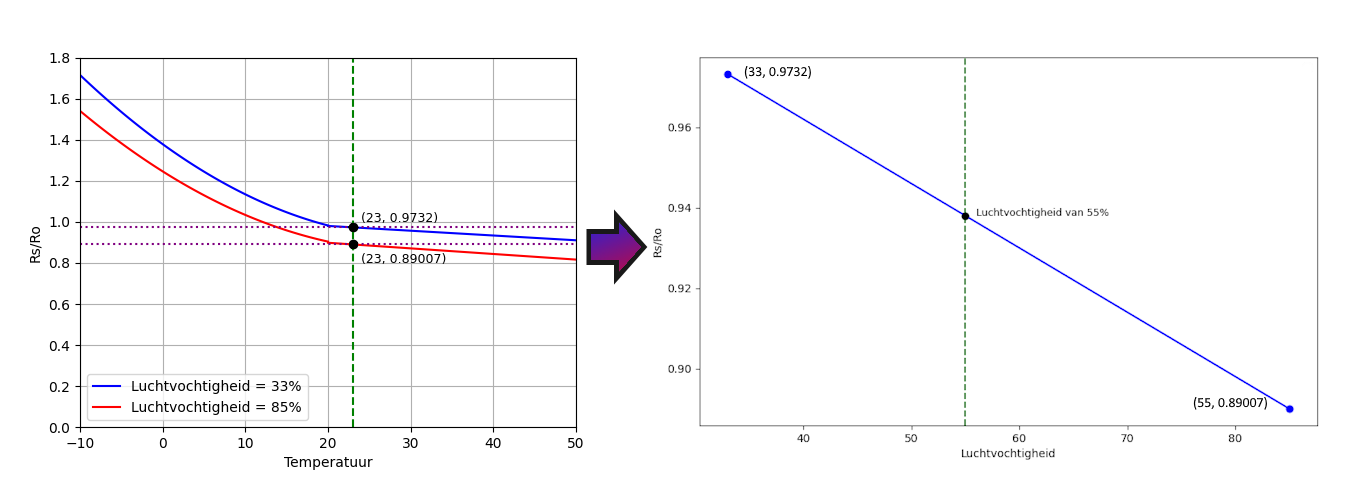
\includegraphics[scale=0.55, center]{berekeningen.png}
    \caption[Voorbeeld berekenen Rs/R0 met temperatuur = 23°C en luchtvochtigheid = 55\%]{Voorbeeld berekenen van de Rs/R0 waarden voor een temperatuur van 23°C en een luchtvochtigheid van 55\%}
    \label{fig:berekeningen}
\end{figure}



%%=============================================================================
%% Methodologie
%%=============================================================================

\chapter{\IfLanguageName{dutch}{Methodologie}{Methodology}}%
\label{ch:methodologie}

%% TODO: In dit hoofstuk geef je een korte toelichting over hoe je te werk bent
%% gegaan. Verdeel je onderzoek in grote fasen, en licht in elke fase toe wat
%% de doelstelling was, welke deliverables daar uit gekomen zijn, en welke
%% onderzoeksmethoden je daarbij toegepast hebt. Verantwoord waarom je
%% op deze manier te werk gegaan bent.
%% 
%% Voorbeelden van zulke fasen zijn: literatuurstudie, opstellen van een
%% requirements-analyse, opstellen long-list (bij vergelijkende studie),
%% selectie van geschikte tools (bij vergelijkende studie, "short-list"),
%% opzetten testopstelling/PoC, uitvoeren testen en verzamelen
%% van resultaten, analyse van resultaten, ...
%%
%% !!!!! LET OP !!!!!
%%
%% Het is uitdrukkelijk NIET de bedoeling dat je het grootste deel van de corpus
%% van je bachelorproef in dit hoofstuk verwerkt! Dit hoofdstuk is eerder een
%% kort overzicht van je plan van aanpak.
%%
%% Maak voor elke fase (behalve het literatuuronderzoek) een NIEUW HOOFDSTUK aan
%% en geef het een gepaste titel.

Zoals bij elke studie was de eerste fase een literatuurstudie om informatie te verwerven over het onderwerp. Zo begon dit onderzoek met een literatuurstudie in verband met stalgassen, types sensoren en de werking van de MQ-sensor. Met deze informatie werd aan de slag gegaan en werden de geschikte tools geselecteerd ~\ref{sec:selectie}. Hierna werd een eigen set-up opgezet waarmee de drie sensoren konden worden uitgelezen. Om de PPM waarden te verkrijgen werd onderzocht hoe deze sensors moesten worden gekalibreerd ~\ref{sec:kalibratie}. Vervolgens werd de ESP01 WiFi-module geanalyseerd en geconfigureerd. Parallel hieraan werd ThingSpeak opgezet en de databank gecreëerd ~\ref{sec:verzendendata}. Toen mijn co-promotor Pieter-Jan afkwam met de vraag of ik de warmte-koelcyclus van de MQ-7 eens kon bestuderen leek me dit interessant en heb ik deze geïmplementeerd in mijn set-up ~\ref{sec:warmte_koel}. Met de implementatie van de DHT22 kon de invloed van temperatuur en luchtvochtigheid op de metingen worden berekend ~\ref{sec:dht22}. Tenslotte werden de bekomen resultaten geanalyseerd via PowerBI ~\ref{sec:analysis}.


\section{Selectie van geschikte tools}%
\label{sec:selectie}

Na de literatuurstudie over stalgassen, sensoren en de MQ-sensor, was de volgende stap de selectie van geschikte tools voor de realisatie van het onderzoek. De volgende lijst omvat zowel de hardware- als softwaretools die essentieel waren voor het opzetten van de test set-up.

Hardware:
\begin{itemize}
    \item Arduino Mega: De Arduino Mega diende als microcontroller om de sensoren te besturen, data te verzamelen en te communiceren met de ESP01 WiFi-module.
    \item Breadboard en nodige kabeltjes: Via een breadboard konden alle elektronische componenten worden verbonden zonder te solderen.
    \item De MQ-4, MQ-7 en MQ-135 gassensoren en de DHT22 temperatuurs- en vochtigheidssensor.
    \item 2 weerstanden van 10k$\Omega$ en een MOSFET-transistor van het type IRF2807: Gebruikt om de stroomtoevoer naar de verwarmingselementen van de MQ-7-sensor te regelen.
    \item ESP01 WiFi-module en adapter: Via de ESP01 kon de verzamelde data naar de databank en Thingspeak worden verstuurd, de adapter werd gebruikt om de ESP01 op het breadboard te monteren.
\end{itemize}

Software:
\begin{itemize}
    \item De software naar keuze voor de databank was MySQL, met Apache kon deze worden gehost op een lokale server waardoor deze bereikbaar was voor de ESP01. De verzamelde data kon hierna worden geanalyseerd met PowerBI.
    \item ThingSpeak werd gebruikt als IoT-platform om de live data te visualiseren.
    \item Verder werd nog de Arduino IDE gebruikt voor de Arduino te programmeren en WebPlotDigitizer om de data uit grafieken te halen.
\end{itemize}


\section{Kalibreren van de MQ-sensors}%
\label{sec:kalibratie}

\section{Verzenden van data}%
\label{sec:verzendendata}

\section{Implementatie warmte-koelcyclus}%
\label{sec:warmte_koel}

\section{Implementatie DHT22-sensor}%
\label{sec:dht22}

\section{Analyse van de resultaten}%
\label{sec:analysis}



% Voeg hier je eigen hoofdstukken toe die de ``corpus'' van je bachelorproef
% vormen. De structuur en titels hangen af van je eigen onderzoek. Je kan bv.
% elke fase in je onderzoek in een apart hoofdstuk bespreken.


%%=============================================================================
%% Test set-up
%%=============================================================================

\chapter{Test set-up}%
\label{ch:test_setup}

Dit hoofdstuk biedt een gedetailleerde beschrijving van het proces waarmee de uiteindelijke test set-up tot stand is gekomen. Al de aparte onderdelen worden besproken en vervolgens worden alle componenten samengevoegd tot één werkende test set-up. Elk van de volgende stappen is genoeg gedocumenteerd en kan gemakkelijk gereproduceerd worden door anderen die een vergelijkbare set-up willen maken.

\section{Kalibratie van de sensoren}%
\label{sec:kalibratie}

Om de MQ-sensoren te kalibreren is het zeer belangrijk dat ze voor de eerste keer gebruik een voorverwarmperdiode van 24-48u hebben gehad, hierna volstaat een opwarmperiode van 5 minuten bij elke keer dat ze gebruikt worden. Vervolgens moet de R\textsubscript{0} waarde voor iedere sensor worden berekend, het is belangrijk dat dit gedaan wordt in schone lucht. Sectie~\ref{sec:hoe-luchtsamenstelling meten} kon worden gedaan. In de Arduino functie in bijlage (\ref{lst:kalibratie}) is te zien hoe dit gebeurt volgens de werkwijze in sectie~\ref{sec:hoe-luchtsamenstelling meten}.

Nadat dit script enige tijd heeft gedraaid kan R\textsubscript{0} worden bepaald via het gemiddelde te nemen. In figuur~\ref{fig:avg_van_R0} is te zien hoe dit gemakkelijk kan worden gedaan aan de hand van een SQL-tabel.

\begin{figure}[h]
    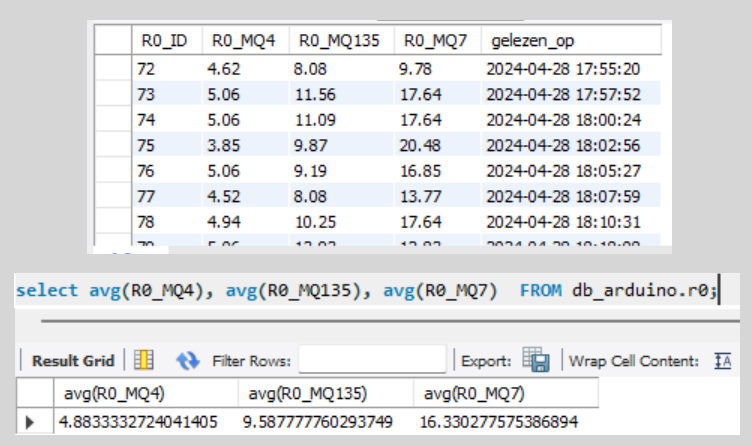
\includegraphics[scale=0.5, center]{avg_van_R0.png}
    \caption[R0 waarden in SQL]{Bepalen van de R0 waarden via SQL}
    \label{fig:avg_van_R0}
\end{figure}

Nu de R\textsubscript{0} waarden zijn bepaald kan er per gas de ppm-waarde worden berekend. In sectie~\ref{sec:hoe-luchtsamenstelling meten} wordt uitgelegd hoe de waarden van de gevoeligheidscurves eerst moeten worden bepaald, en zoals reeds aangehaald wordt dit het best gedaan via een tool zoals WebPlotDigitizer \autocite{Rohatgi2024}. Hier kan een grafiek worden ingeladen waarna de x- en y-as moeten worden uitgelijnd, het is belangrijk dat deze assen worden ingesteld als logaritmisch (zie figuur~\ref{fig:x_en_y}). Vervolgens moeten er per gas 2 punten worden aangeduid, die liefst zo ver mogelijk van elkaar liggen (figuur~\ref{fig:voorbeeld}).

\begin{figure}[h]
    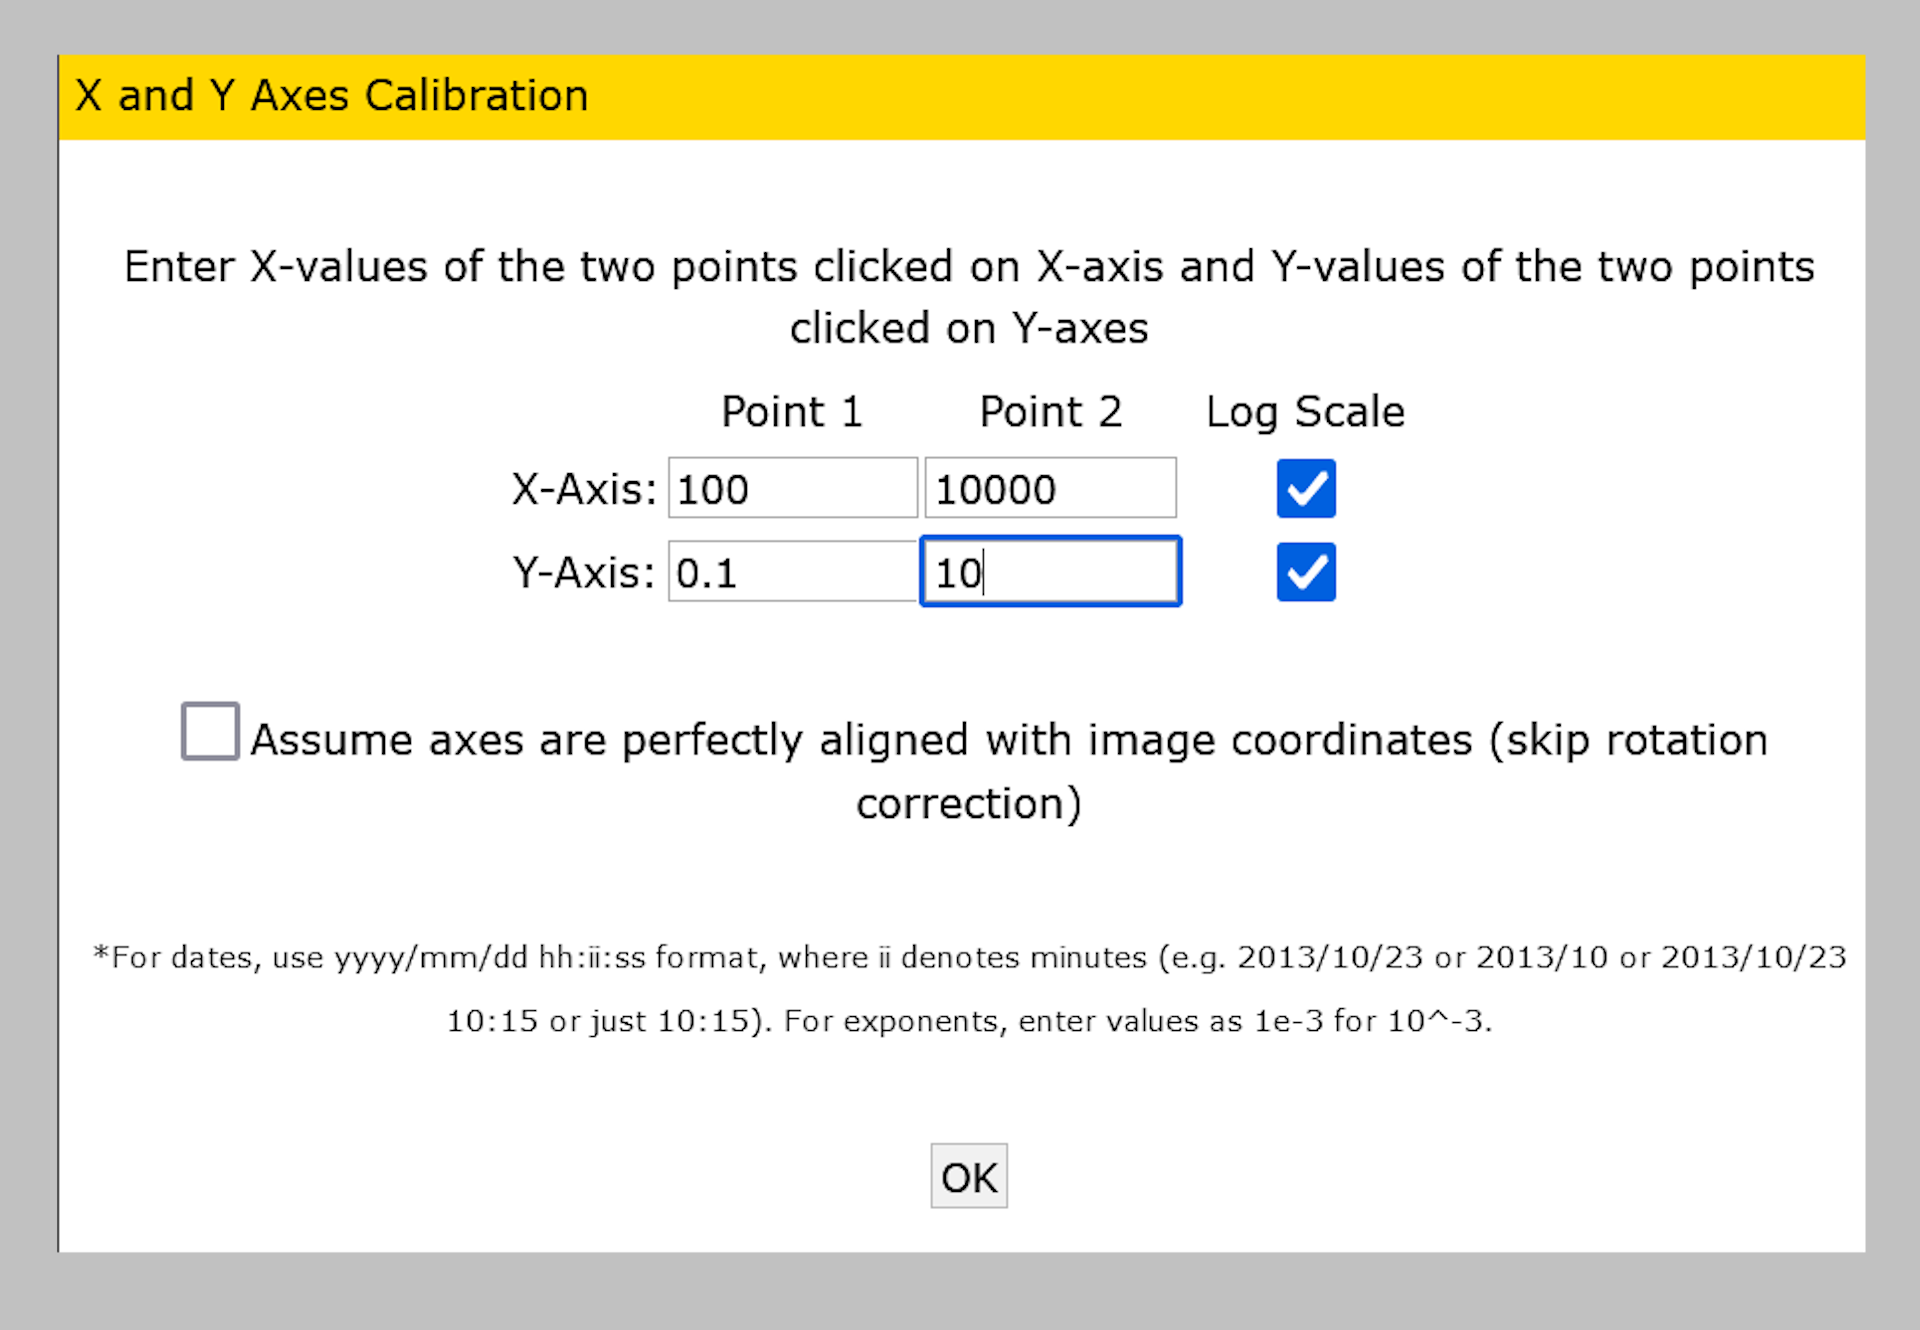
\includegraphics[scale=0.25, center]{XenY.png}
    \caption[Uitlijnen X- en Y-assen]{Uitlijnen van de X- en Y-assen in WebPlotDigitizer}
    \label{fig:x_en_y}
\end{figure}

\begin{figure}[h]
    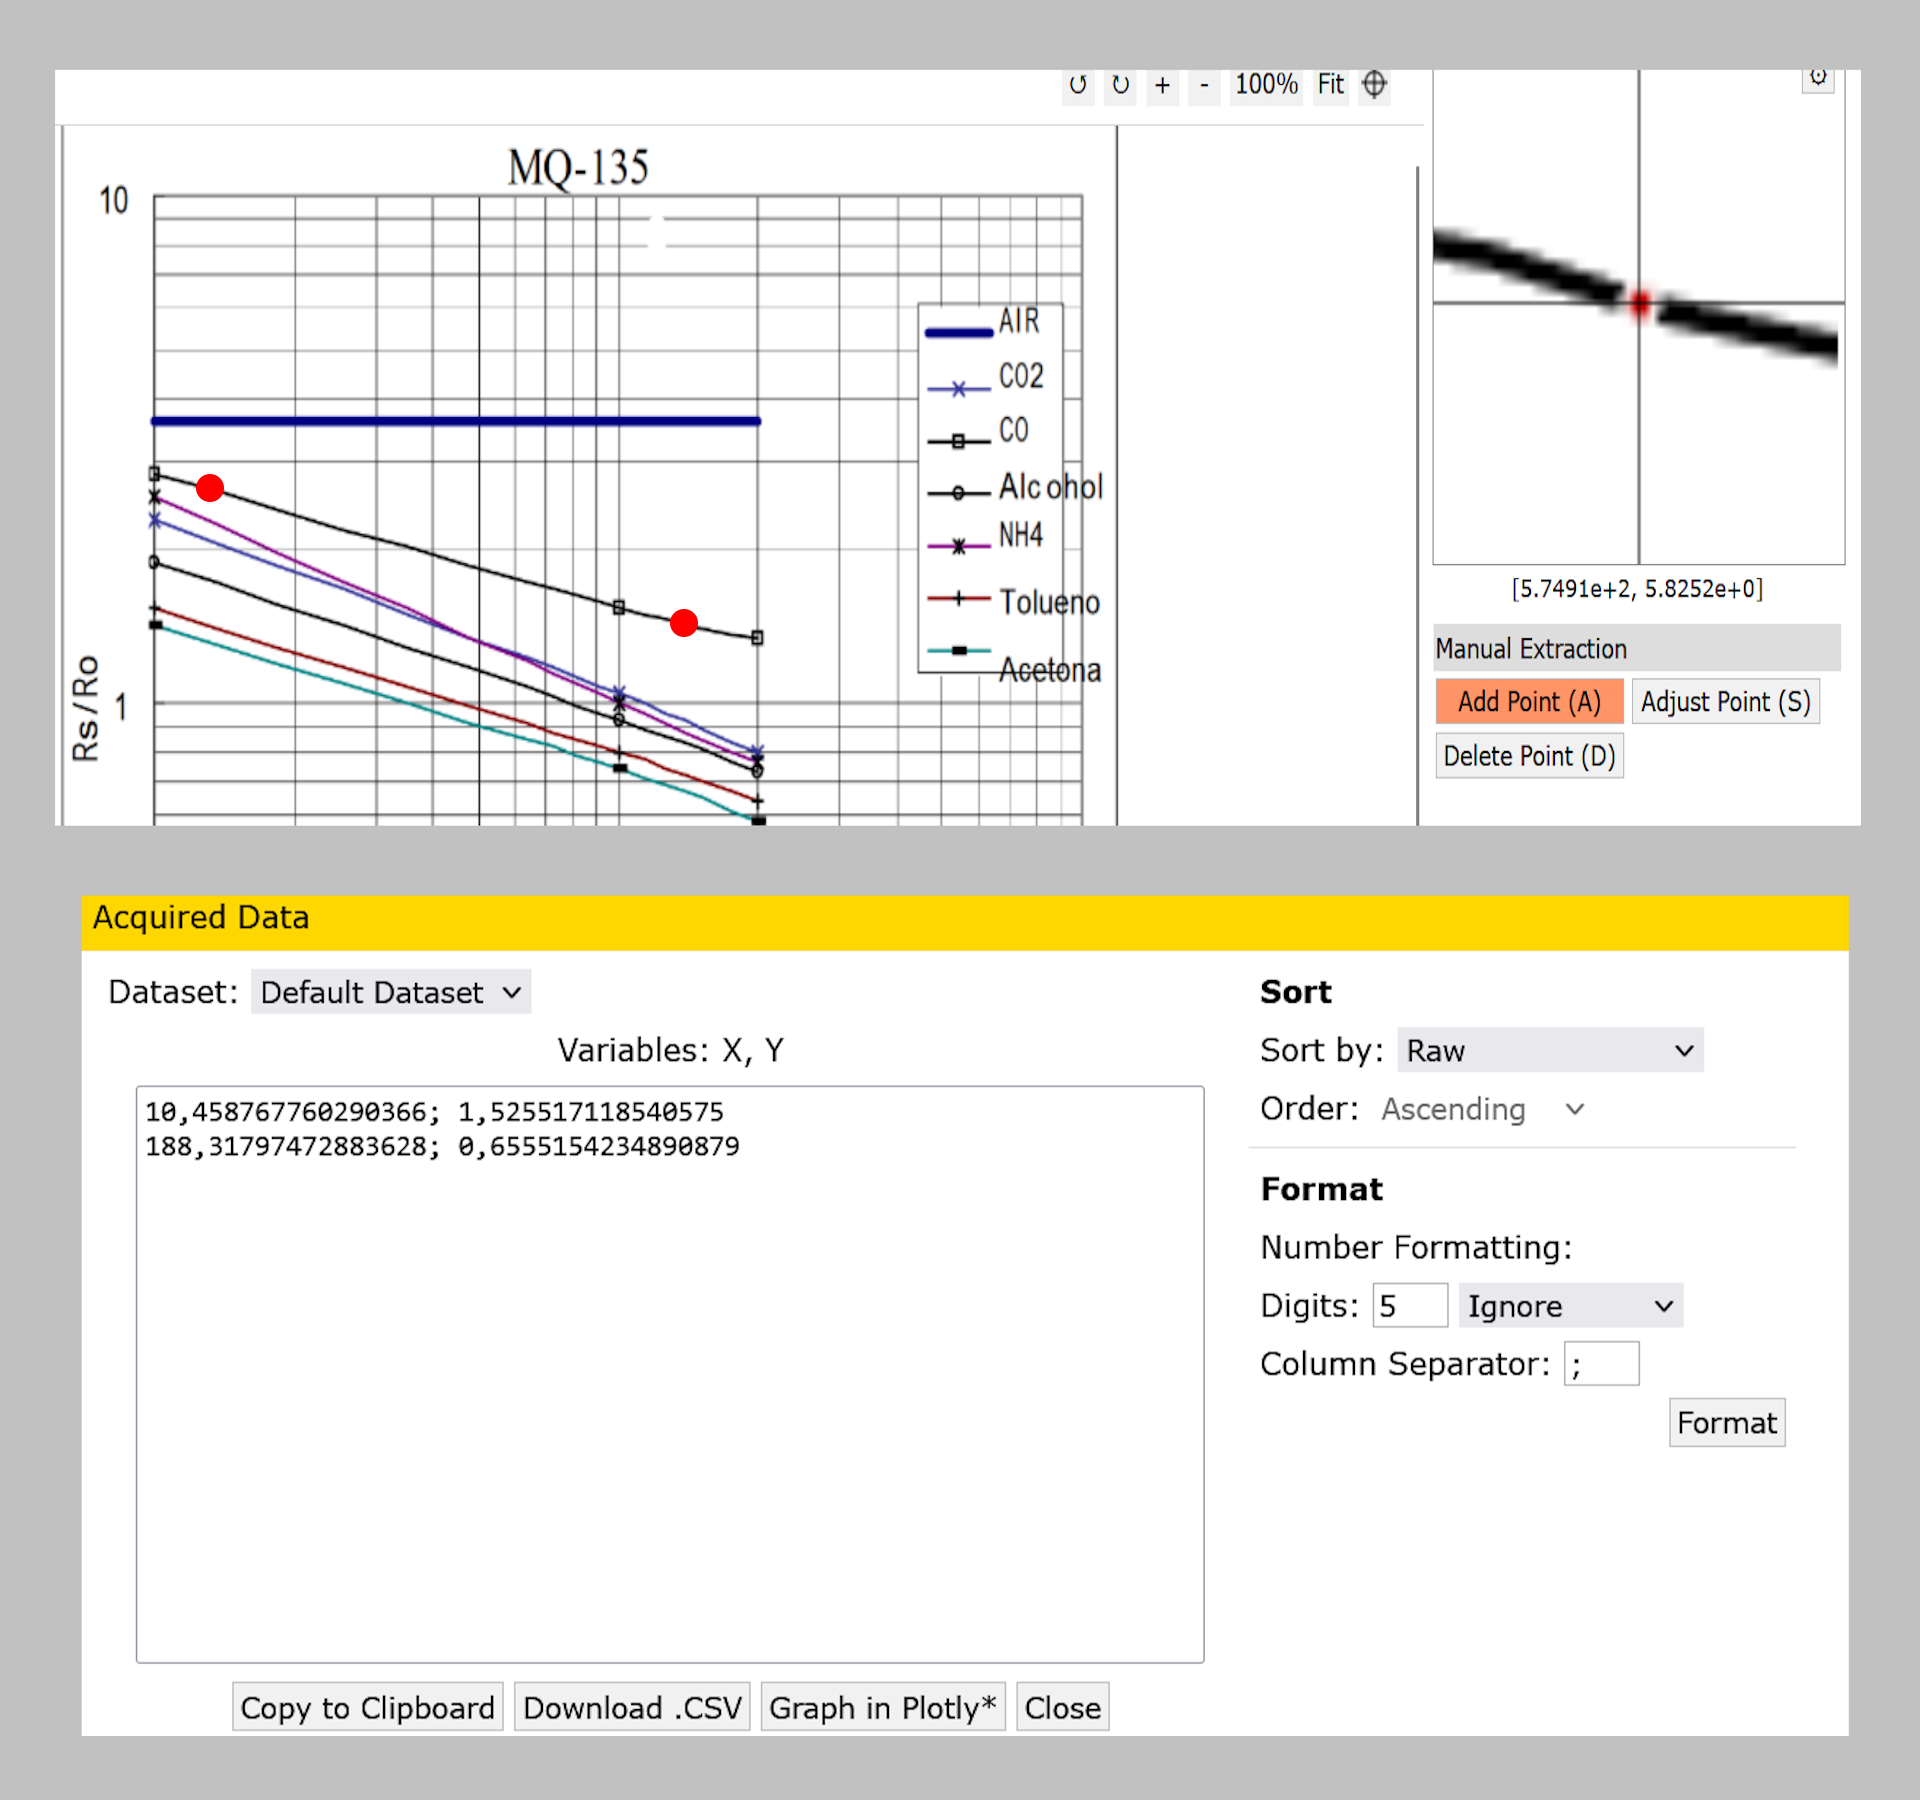
\includegraphics[scale=0.25, center]{voorbeeld.png}
    \caption[Datapunten uit WebPlotDigitizer]{Verkrijgen van de datapunten uit de grafiek in WebPlotDigitizer}
    \label{fig:voorbeeld}
\end{figure}

Met deze waarden kan er vervolgens worden verdergegaan. Zo zie je in script~\ref{lst:ppm_mq135} hoe op deze manier de ppm voor alle gassen van de MQ-135 sensor worden berekend.

\pagebreak

\section{Verzenden van data}%
\label{sec:verzendendata}

Het verzenden van deze data gebeurt met een ESP8266-01s, of in het kort de ESP01. Zoals reeds besproken in sectie~\ref{subsec:esp01} werkt deze WiFi module met AT-commando's. Vooraleer de ESP01 kan worden gebruikt moeten er een paar stappen gebeuren. Zo moet de juiste firmware geïnstalleerd worden, dit wordt besproken in sectie~\ref{subsec:firmware} van de bijlage. Hiernaast moet de ESP01 juist worden ingesteld via AT commando's, dit is stap voor stap te zien in sectie~\ref{subsec:instellen} in de bijlage.

Nadat de voorafgaande stappen zijn gebeurd kan de ESP01 worden aangesproken in de code zelf, en niet enkel in de command-line-interface van de Arduino IDE. De ESP-module wordt als volgt geïnitialiseerd:
\begin{lstlisting}[language=Java, caption={Initialisatie van de ESP in Arduino}]
#include <SoftwareSerial.h>
#include <stdlib.h>

SoftwareSerial ESP(10, 11); // TX, RX
ESP.begin(9600); // baud rate van 9600
\end{lstlisting}

Vervolgens worden AT commando's gestuurd via:
\begin{lstlisting}[language=Java, caption={Voorbeeld: resetten van de ESP}]
ESP.println("AT+RST");
\end{lstlisting}

\subsection{Verzenden naar Thingspeak}
\label{subsec:thingspeak}

Het Thingspeak platform is volledig open-source. Gebruikers kunnen gratis kanalen aanmaken waarnaar data kan worden geschreven die live wordt getoond. Om data te uploaden moet gebruik worden gemaakt van het IP adres van Thingspeak (184.106.153.149) en de API Write key van het kanaal waar de data op zal worden vertoond.

In Thingspeak zelf kunnen tot 8 velden worden ingesteld. Figuur~\ref{tab:velden} toont welke veld zijn gebruikt in dit project.
\begin{table}[h]
    \centering
    \begin{tabular}{|c|c|}
        \hline
        Veld & Beschrijving \\
        \hline
        1 & MQ135\_CO2 \\
        2 & MQ135\_NH4 \\
        3 & MQ7\_CO \\
        4 & MQ4\_CH4 \\
        5 & MQ7\_H2 \\
        6 & MQ4\_LPG \\
        7 & Temperatuur \\
        8 & Luchtvochtigheid \\
        \hline
    \end{tabular}
    \caption{Velden in Thingspeak}
    \label{tab:velden}
\end{table}

Om data te versturen via de ESP01 moeten de de volgende commando's naar de WiFi module worden verstuurd:
\begin{lstlisting}[language=Java,caption={ESP01 naar Thingspeak}]
AT+CIPSTART="TCP","184.106.153.149",80  // verbinding maken met Thingspeak via TCP
    CONNECT
    OK

AT+CIPSEND=49   // lengte van het bericht
    OK

> GET /update?key={API_WRITE_KEY}&field1=X&field2=Y //waarde X naar field1 en waarde Y naar field2 versturen
    SEND OK

AT+CIPCLOSE  //verbinding sluiten
    OK
\end{lstlisting}

Hierna worden deze waarden toegevoegd aan Thingspeak. Het visualiseren van de data kan via de standaard visualisaties van Thingspeak, maar voor meer controle kunnen er via Matlab \autocite{MATLAB} eigen visualisaties worden gemaakt. De Matlab code in sectie~\ref{sec:matlab} van de bijlage toont aan hoe al de velden op 1 scherm kunnen worden getoond.
Het uiteindelijke resultaat is te zien is figuur~\ref{fig:matlab}:

\begin{figure}[h]
    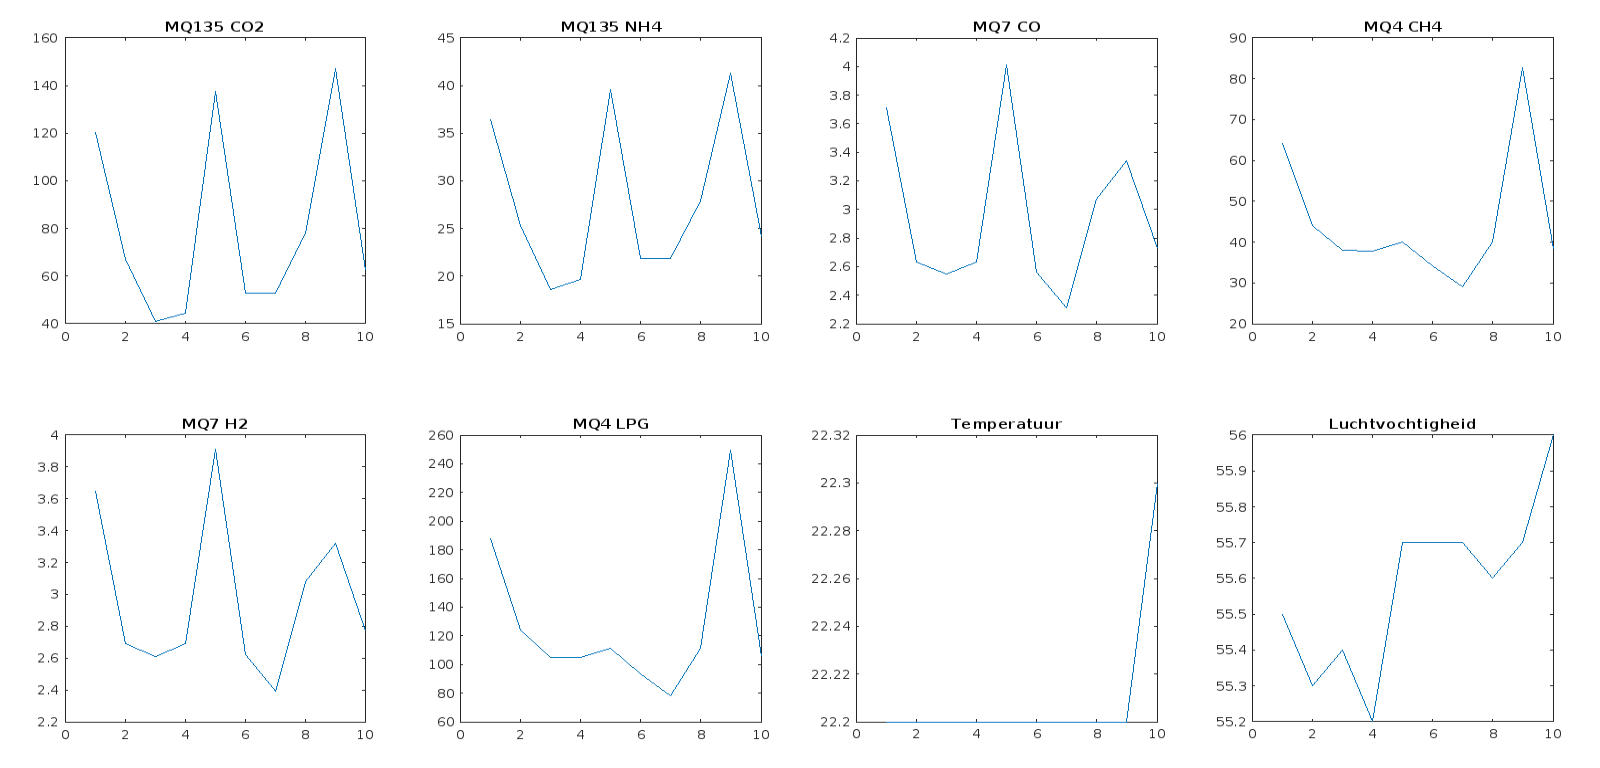
\includegraphics[scale=0.5, center]{matlab.png}
    \caption[Thingspeak live]{Een live weergave van de waarden van de MQ-sensoren via Thingspeak}
    \label{fig:matlab}
\end{figure}


\subsection{Verzenden naar databank}
\label{subsec:database}

Om de data te kunnen analyseren via PowerBI is het essentieel dat ze ook naar een databank kan worden verstuurd. Deze databank werd opgezet via MySQL (\ref{fig:SQLtabellen}). Zo kreeg iedere MQ-sensor een eigen tabel met al hun gasmetingen en een datetime-object die aantoont wanneer dit gelezen is. Ook is er een DHT22 tabel, waar de temperatuur en luchtvochtigheid worden opgeslagen. Verder is er nog een tabel voor de R\textsubscript{0} waarden en voor de analoge waarden van de MQ7, deze zal verder worden besproken in sectie~\ref{sec:warmte_koel}.

\begin{figure}[h]
    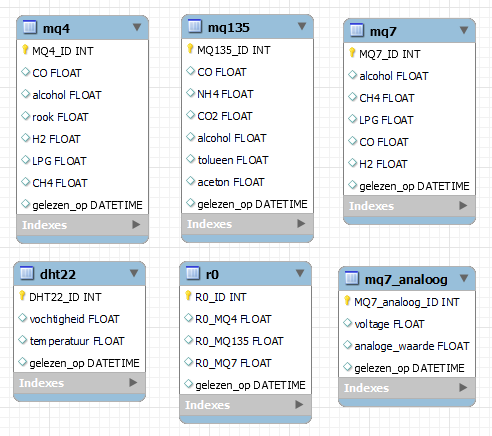
\includegraphics[scale=0.9, center]{SQLtabellen.png}
    \caption[Tabellen in de databank]{Tabellen in de MySQL databank}
    \label{fig:SQLtabellen}
\end{figure}

Deze databank wordt gehost met Apache, de ESP01 en de hostcomputer moeten dus op hetzelfde netwerk zitten. Hoe Apache werd ingesteld is te vinden in bijlage~\ref{sec:database}. Om de waarden daadwerkelijk in de databank te krijgen moet gebruik worden gemaakt van PHP scripts. In deze scripts wordt er een connectie gemaakt met de databank en worden de waarden via SQL-statements in de juiste tabel gegoten. In de volgende listing is een voorbeeld te zien van het PHP-script voor de gasmetingen van de MQ-135:
\begin{lstlisting}[language=PHP,caption={PHP-script MQ-135}]
<?php

$MQ135_CO_ppm = $_POST["MQ135_CO_ppm"];
$MQ135_NH4_ppm = $_POST["MQ135_NH4_ppm"];
$MQ135_CO2_ppm = $_POST["MQ135_CO2_ppm"];
$MQ135_alcohol_ppm = $_POST["MQ135_alcohol_ppm"];
$MQ135_tolueen_ppm = $_POST["MQ135_tolueen_ppm"];
$MQ135_aceton_ppm = $_POST["MQ135_aceton_ppm"];


$servername = "localhost";
$username = "root";
$password = "root";
$dbname = "db_arduino";

// Create connection
$conn = new mysqli($servername, $username, $password, $dbname);
// Check connection
if ($conn->connect_error) {
    die("Connection failed: " . $conn->connect_error);
}

$sql = "INSERT INTO MQ135 (CO, NH4, CO2, alcohol, tolueen, aceton, gelezen_op) VALUES ($MQ135_CO_ppm, $MQ135_NH4_ppm, $MQ135_CO2_ppm, $MQ135_alcohol_ppm, $MQ135_tolueen_ppm, $MQ135_aceton_ppm, NOW())";
if ($conn->query($sql) === TRUE) {
    echo "New record created successfully";
} else {
    echo "Error: " . $sql . " => " . $conn->error;
}


$conn->close();

?>

\end{lstlisting}

Als de databank is opgezet, de PHP-scripts zijn geschreven en Apache runt kunnen met behulp van de volgende AT-commando's waarden worden toegevoegd aan de databank:
\begin{lstlisting}[language=Java,caption={ESP01 naar de database}]
AT+CIPSTART="TCP","192.168.1.44",80  //lokale IP adres van de host
    CONNECT
    OK

AT+CIPSEND=236  //grootte van het bericht
    OK
    
> POST /insertMQ4DB.php HTTP/1.1    //naam php script
  Host: 192.168.1.44
  Connection: keep-alive
  Content-Type: application/x-www-form-urlencoded
  Content-Length: 86

  MQ4_CO_ppm=1&MQ4_alcohol_ppm=2&MQ4_rook_ppm=3&MQ4_H2_ppm=4&MQ4_LPG_ppm=5&MQ4_CH4_ppm=6

    SEND OK
    
    +IPD,285:HTTP/1.1 200 OK
    Date: Tue, 2 Apr 2024 14:54:11 GMT
    Server: Apache/2.4.58 (Win64) OpenSSL/3.1.3 PHP/8.2.12
    X-Powered-By: PHP/8.2.12
    Content-Length: 31
    Keep-Alive: timeout=5, max=100
    Connection: Keep-Alive
    Content-Type: text/html; charset=UTF-8
    New record created successfully

    CLOSED
    
\end{lstlisting}


\section{Implementatie van de warmte-koelcyclus}%
\label{sec:warmte_koel}


Zoals besproken in sectie~\ref{sec:warmte-koelcyclus} is het werkingsprincipe van de MQ-7 sensor anders dan de andere sensoren. Voor optimale resultaten moet er  gebruik worden gemaakt van een warmte-koelcyclus. In het onderzoek van \textcite{Kobbekaduwa2021} wordt duidelijk uitgelegd hoe deze warmte-koelcyclus kan worden geïmplementeerd. 

In figuur~\ref{fig:heatcool_circuit} wordt aangetoond aan hoe het circuit diagram uit moet uit zien volgens \textcite{Kobbekaduwa2021}.

\begin{figure}[h]
    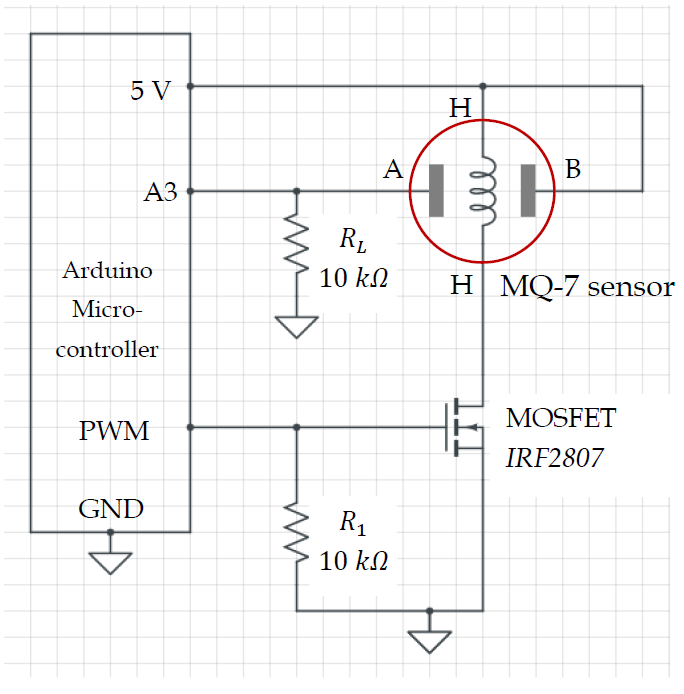
\includegraphics[scale=0.3, center]{heatcool_circuit.png}
    \caption[Circuit warmte-koelcyclus]{Het circuit voor een warmte-koelcyclus \autocite{Kobbekaduwa2021}}
    \label{fig:heatcool_circuit}
\end{figure}

In dit circuit is te zien hoe de opwarming van de MQ-7 sensor gebeurt. De Arduino stuurt de MOSFET transistor aan om zo het voltage van de MQ-7 te veranderen. De MQ-7 moet 60 seconden lang 5V toegediend krijgen om alle gassen te verdampen en de sensor te reinigen. Hierna krijgt de sensor 90 seconden lang 1.4V toegediend, hier worden de gassen gemeten. De volgende listing toont aan hoe kan worden gedaan in Arduino code volgens de werkwijze van \textcite{Kobbekaduwa2021}:

\begin{lstlisting}[language=Java,caption={Warmte-koelcyclus MQ-7}]
//pinnen vd sensoren 
int MQ7 = A2;
int mosfet = 9;

void setup() {
    Serial.begin(9600);
    pinMode(MQ7, INPUT);
    pinMode(mosfet, OUTPUT);
}

void loop() {
    // MQ7 hoog (voor 60 sec)
    analogWrite(mosfet, 255); //5V naar MQ7
    delay(60000);
    // MQ7 laag (voor 90 sec)
    analogWrite(mosfet, 72); //1.4V naar MQ7
    delay(90000);
    
    Serial.println(analogRead(MQ7));
}
        
\end{lstlisting}

Nu dit geïmplementeerd is kunnen deze waarden ook naar de database worden gestuurd voor een analyse. De grafiek (zoals bijvoorbeeld die van figuur~\ref{fig:mq7_heatcool_vb}) die ontstaat tijdens deze cyclus roept vragen op zoals: zijn verschillende gassen te onderscheiden in deze grafiek? En welke invloed hebben de temperatuur en vochtigheidsgraad?

\begin{figure}[h]
    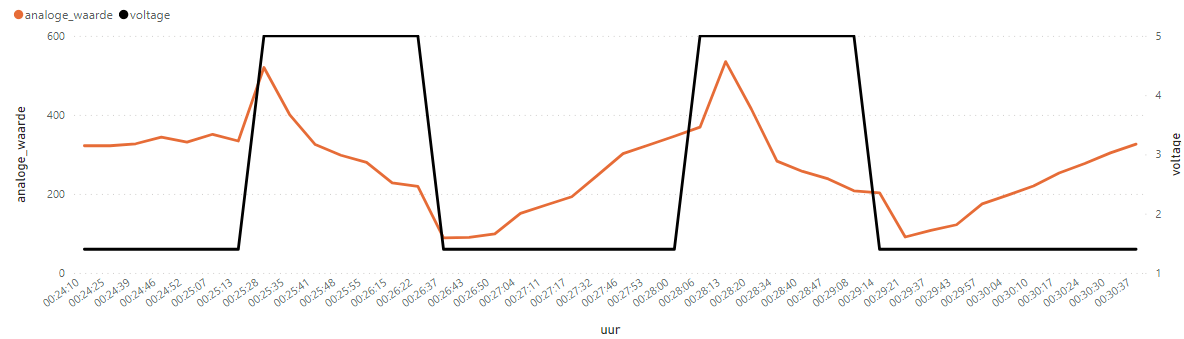
\includegraphics[scale=0.5, center]{mq7_heatcool_vb.png}
    \caption[Warmte-koelcyclus in de praktijk]{Voorbeeld van de visualisatie van de warmte-koelcyclus}
    \label{fig:mq7_heatcool_vb}
\end{figure}


Omdat dit interessante zaken kunnen zijn voor een analyse zijn ze getest geweest. Zo zijn er experimenten opgezet met 3 verschillende gassen waar de MQ-7 gevoelig voor is: CO, alcohol en LPG. Deze experimenten zijn uitgevoerd in een normale omgeving en een omgeving met een hoge vochtigheidsgraad.

%Een van de hoofdbestanddelen van rook is koolstofmonoxide, zo werd er door de rook van een brandende lucifer een hoge ppm CO gesimuleerd. Zo is er voor alcohol de damp van ontsmettingsalcohol gebruikt, en voor LPG de damp van aanstekerbenzine. De experimenten in normale omgeving werden buiten uitgevoerd, en voor de hoge vochtigheidsgraad is er in een vochtige badkamer gewerkt.

Omdat de ESP01 module niet snel genoeg data kan versturen, werd tijdens het experiment om de 2 seconden data geprint in de vorm van INSERT-statements in de Arduino IDE. Hierna kon deze output worden uitgevoerd in MySQL. Op deze manier is er meer detail uit te lezen op de grafieken. Deze resultaten worden besproken in sectie~\ref{sec:analyse_mq7}.




\section{Implementatie van de DHT22-sensor}%
\label{sec:dht22}


Om de DHT22-sensor te implementeren werd gebruik gemaakt van de DHT library op Arduino. Via deze library kan gemakkelijk de temperatuur en luchtvochtigheid worden afgelezen. De DHT22 is een stabiele en nauwkeurige sensor die geen kalibratie nodig heeft.

Om de correctiefactor te implementeren werd de werkwijze beschreven in sectie~\ref{sec:temp-en-hum} geïmplementeerd in de code. De volgende listing toont de functie bereken\_correctiefactor. Hier wordt er op basis van het sensortype, de temperatuur en de luchtvochtigheidsgraad berekent hoeveel de correctiefactor bedraagt.

\begin{lstlisting}[language=Java,caption={Berekenen van de correctiefactor}]
float bereken_correctiefactor(int sensor, float temp, float hum) {
    float y_33;
    float y_85;
    if (temp > 20) {
        switch (sensor) {
            case 4:
            y_33 = -0.00296 * temp + 1.05336;
            y_85 = -0.00434 * temp + 0.93704;
            break;
            case 7:
            y_33 = -0.00442 * temp + 1.08514;
            y_85 = -0.00398 * temp + 0.93537;
            break;
            case 135:
            y_33 = -0.00233 * temp + 1.02679;
            y_85 = -0.00273 * temp + 0.95286;
            break;
            default:
            Serial.println("Foute sensor");
            break;
        }
    } else {
        switch (sensor) {
            case 4:
            y_33 = 0.00022 * pow(temp,2) - 0.01178 * temp + 1.14896;
            y_85 = 0.00012 * pow(temp,2) - 0.00940 * temp + 0.99210;
            break;
            case 7:
            y_33 = 0.00046 * pow(temp,2) - 0.01945 * temp + 1.21352;
            y_85 = 0.00021 * pow(temp,2) - 0.01249 * temp + 1.02743;
            break;
            case 135:
            y_33 = 0.00046 * pow(temp,2) - 0.02907 * temp + 1.37849;
            y_85 = 0.00041 * pow(temp,2) - 0.02534 * temp + 1.24596;
            break;
            default:
            Serial.println("Foute sensor");
            break;
        }
    }
    return y_33 + ((y_85-y_33)/(85-33))*(hum-33);
}
\end{lstlisting}


\section{Finale code}%
\label{sec:final}

De finale code bestaat uit 4 scripts. In de eerste wordt de R\textsubscript{0} waarde berekent en naar de databank verstuurd (\ref{subsec:script_R0}), hier is de warmte-koelcyclus van de MQ-7 ook in opgenomen. In het tweede script wordt de data live naar Thingspeak geüpload (\ref{subsec:script_thingspeak}) en in het derde naar de databank (\ref{subsec:script_db}). Het vierde script werd gebruikt voor de testen met de MQ-7 sensor (\ref{subsec:script_mq7}).

Al deze scripts kunnen worden uitgevoerd met het circuit afgebeeld in figuur~\ref{fig:arduino_circuit}.


\begin{figure}[h]
    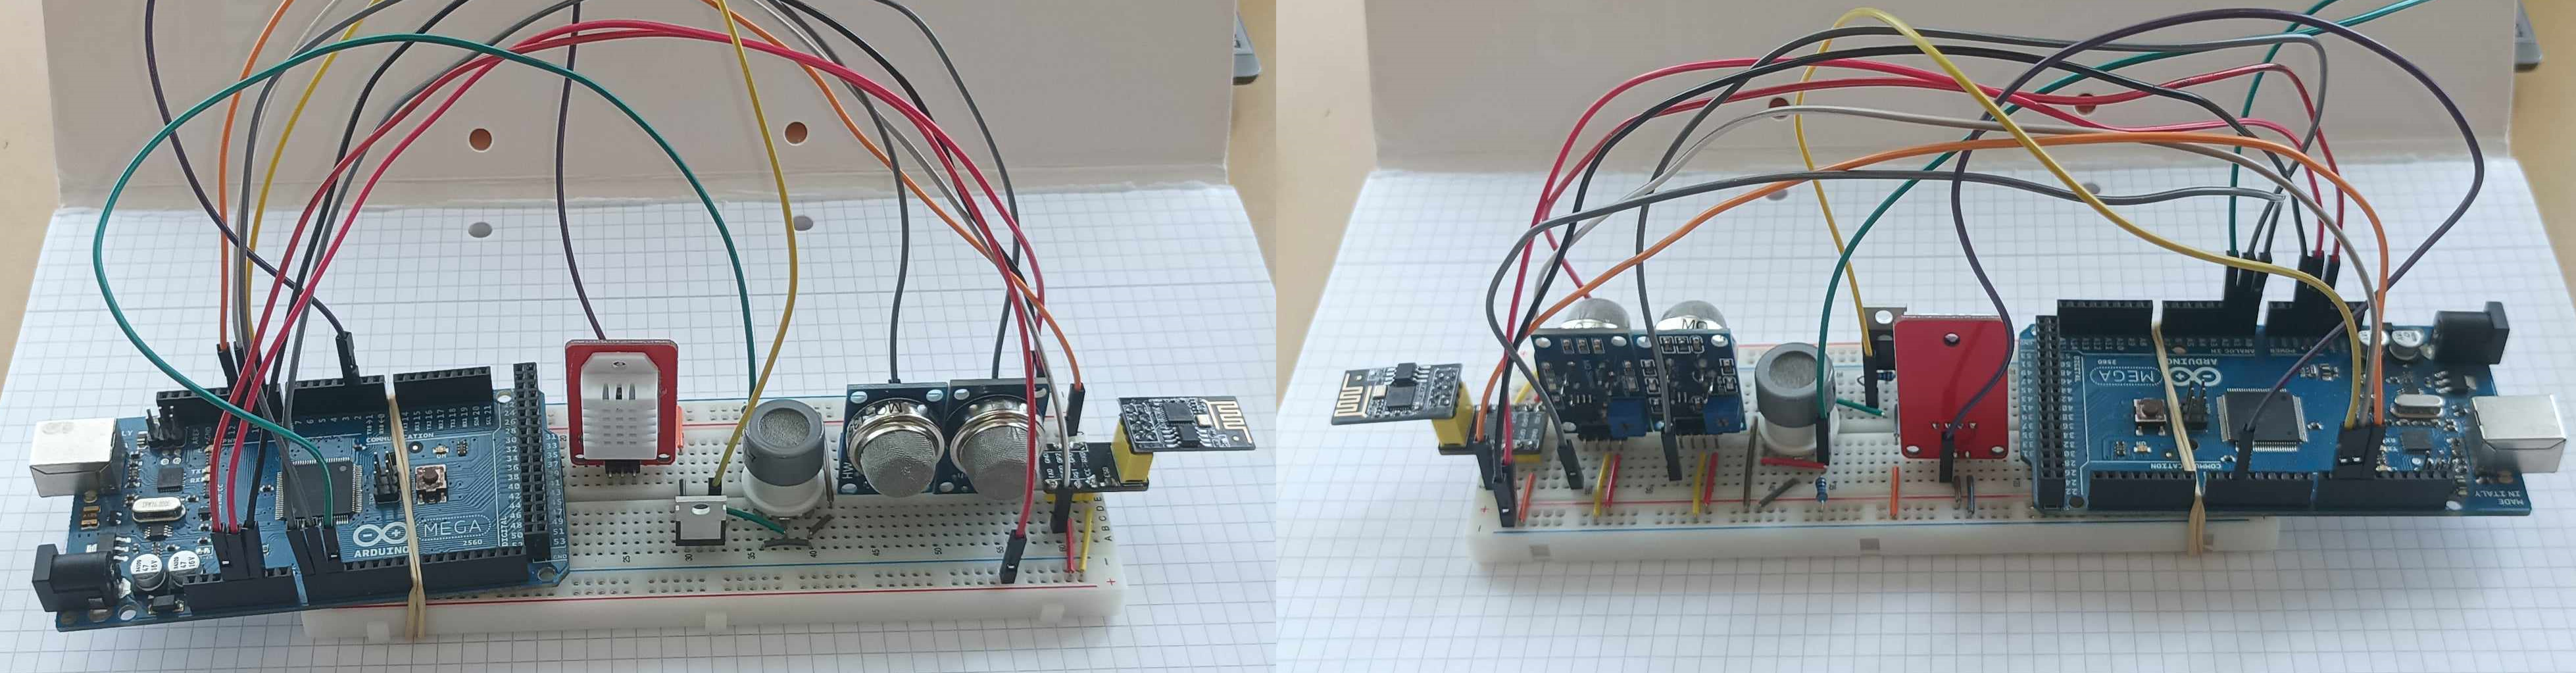
\includegraphics[scale=0.16, center]{voor_en_achterkant.png}
    \caption[Foto test set-up]{Voor- en achterkant van de test set-up}
    \label{fig:voor_en_achterkant}
\end{figure}

\begin{figure}[h]
    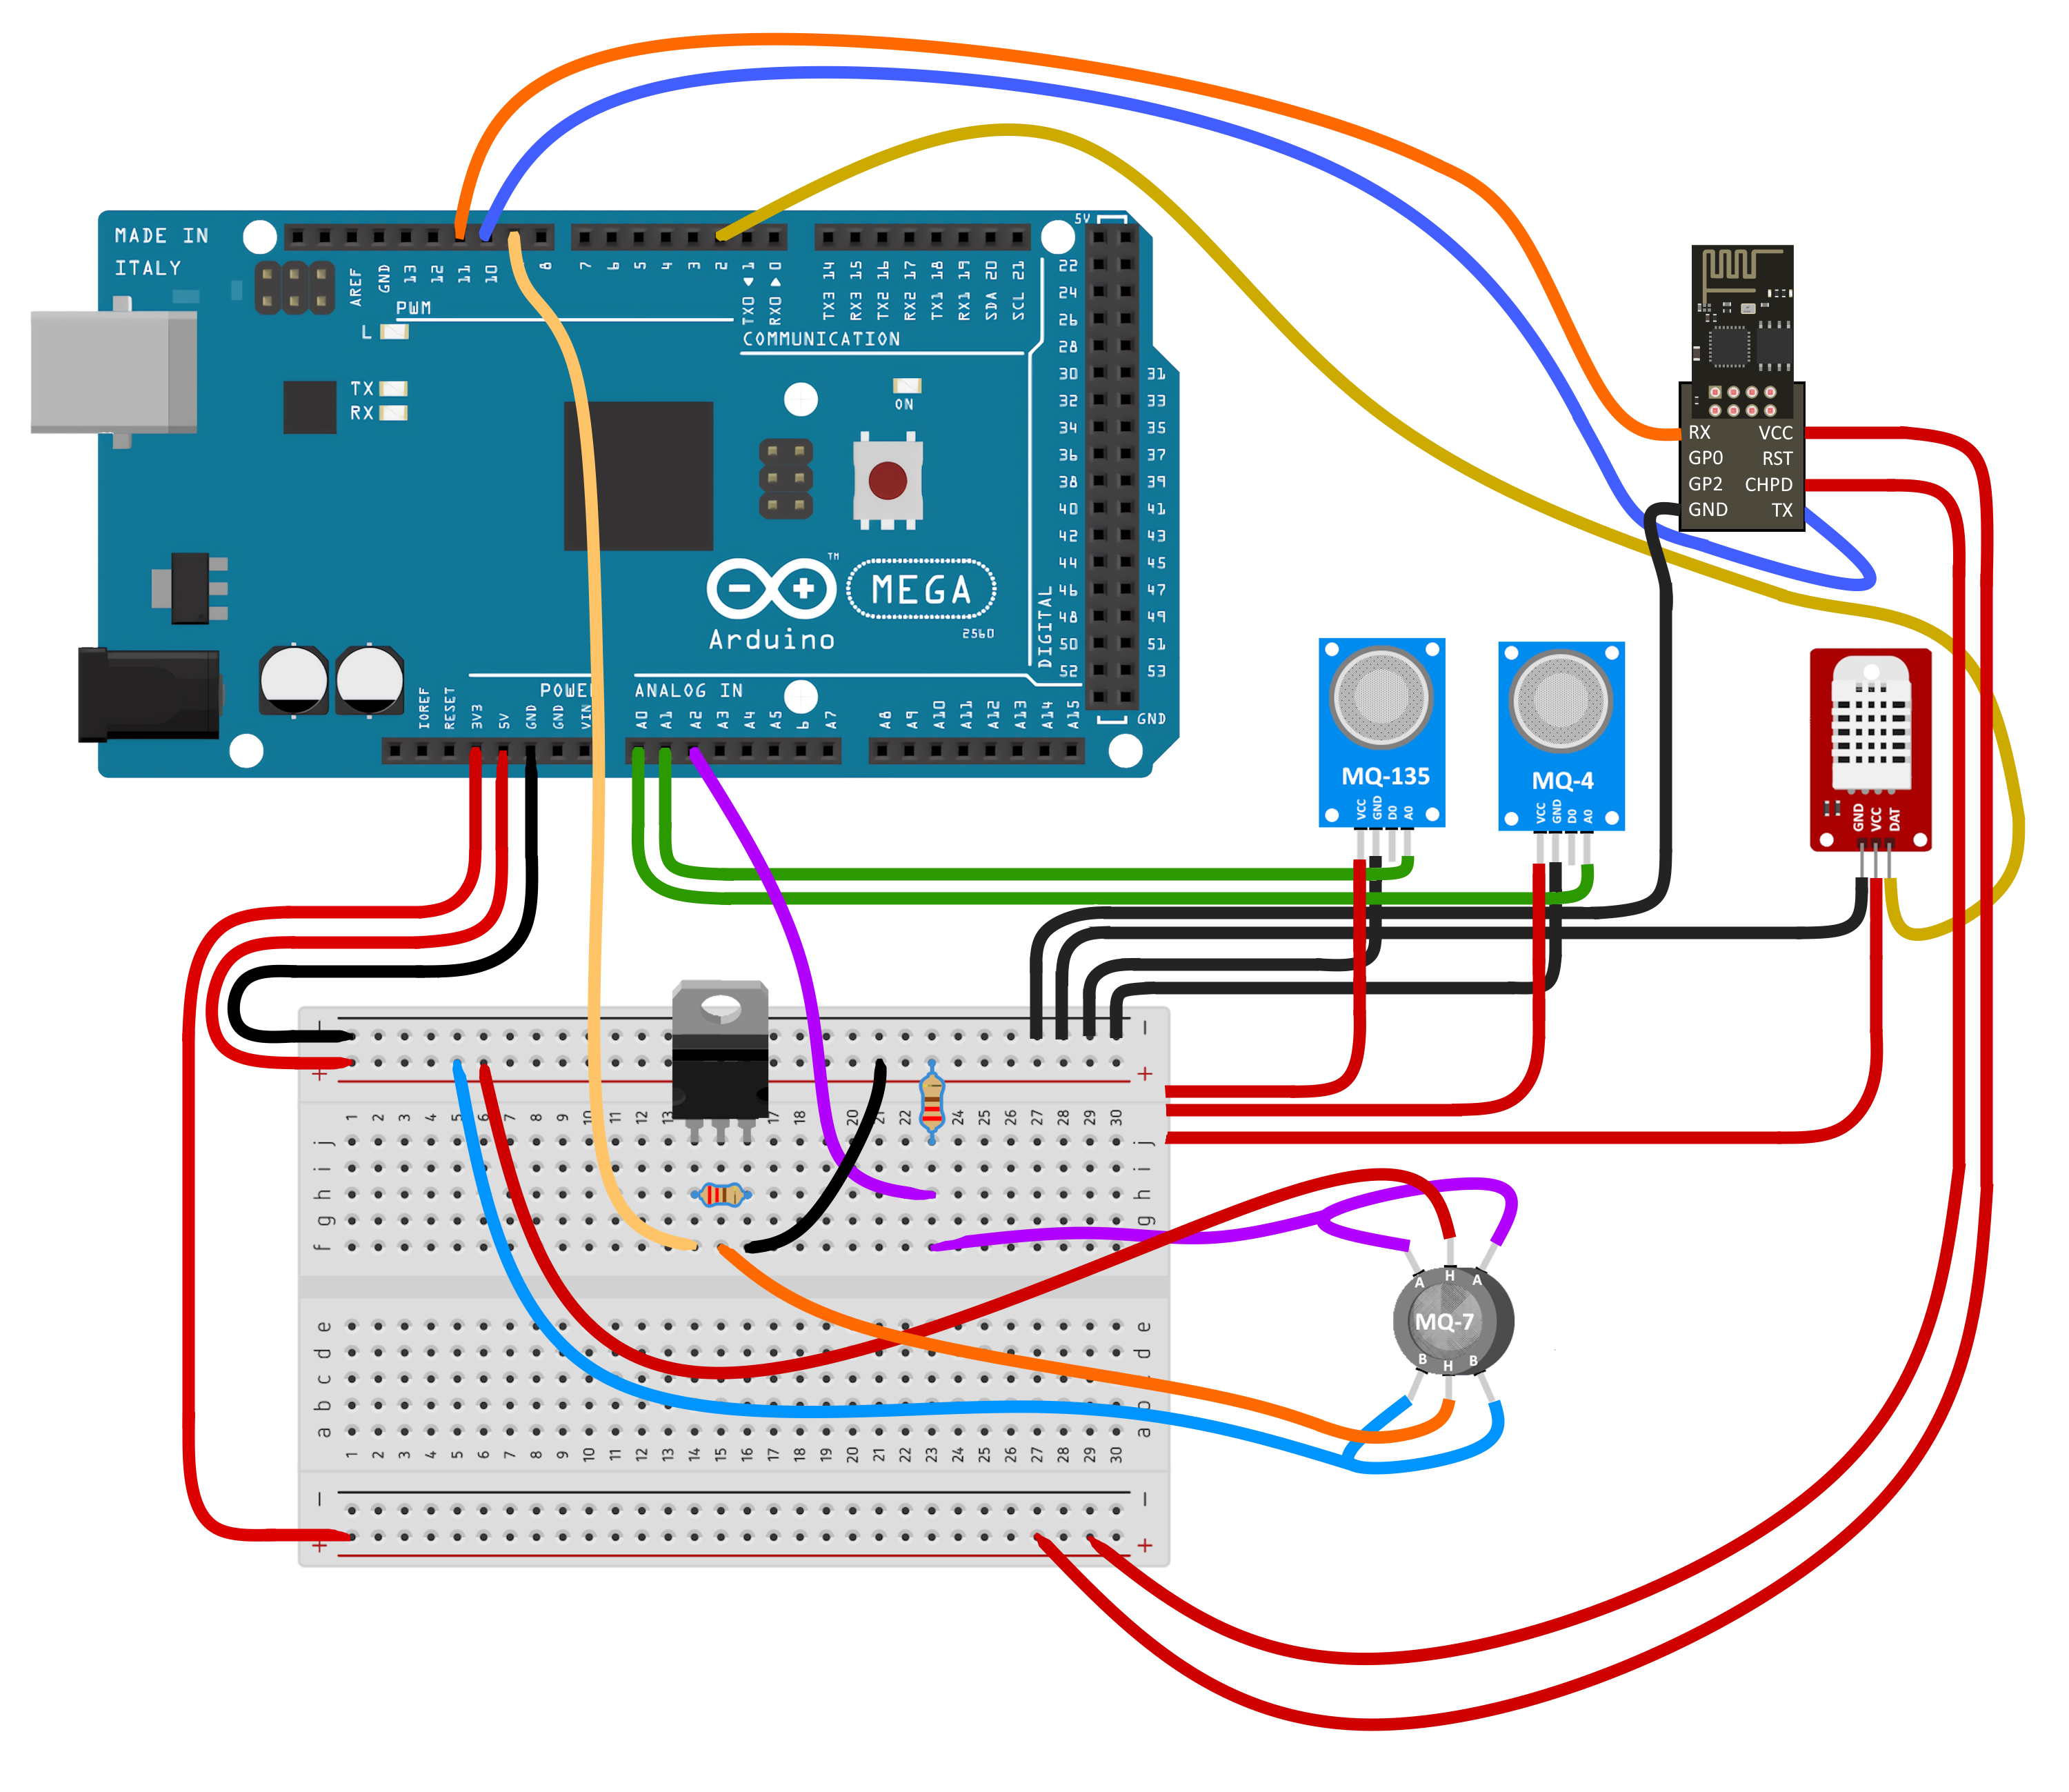
\includegraphics[scale=0.16, center]{arduino_circuit.png}
    \caption[Circuit test set-up]{Finale circuit van de test set-up}
    \label{fig:arduino_circuit}
\end{figure}

\pagebreak

Deze test set-up werd uiteindelijk getest in een kalibratiesetup van ILVO. In deze set-up worden andere gassensoren gekalibreerd die vervolgens worden opgehangen in stallen. Indien deze sensoren geen correcte resultaten geven kunnen ze zo worden bijgesteld. Zo zijn er 2 testen uitgevoerd, een met ammoniak en een met koolstofdioxide. Bij deze kalibratie zitten al de gassensoren in een luchtdichte kist waar gekende gasconcentraties naartoe worden gestuurd. Deze gasconcentraties worden terwijl ook geanalyseerd door een Picarro gassensor. Dit is een zeer nauwkeurige gassensor met een prijskaartje van 150.000€. De Picarro gassensor werkt op basis van een infraroodlaser en kan N\textsubscript{2}O, CH\textsubscript{4}, NH\textsubscript{3} en CO\textsubscript{2} meten.

In de eerste test werd NH\textsubscript{3} aangeboden, dit was interessant om te testen omdat NH\textsubscript{3} een veelvoorkomende en gevaarlijk stalgas is. In de gevoeligheidsgrafieken van de 3 MQ-sensoren staat geen NH\textsubscript{3}, zo werd dus getest of de sensoren daadwerkelijk geen NH\textsubscript{3} konden meten. En indien dit wel lukte, welke sensor hier het beste op reageerde. De NH\textsubscript{3} werd toegediend in 5 fases, in de eerste fase werd een half uur lang niks aangeboden. Daarna werd 1, 3 en 5 ppm NH\textsubscript{3} per anderhalf uur toegediend. In de laatste fase werd terug voor een half uur 0 ppm aangeboden om te testen hoe snel de sensoren terug zouden stabiliseren.

In de tweede test werd CO\textsubscript{2} aangeboden, hier werd vooral getest hoe accuraat de MQ-135 is die CO\textsubscript{2} meet. Maar ook werd getest hoe hard de andere sensoren hier op reageerden. Tijdens deze test is er in 3 fases gewerkt. Zo werd om het uur per fase 0 ppm, 500 ppm en 2000 ppm CO\textsubscript{2} aangeboden.

De resultaten van deze twee testen worden besproken in sectie~\ref{sec:nauwkeurigheid}.

\begin{figure}[h]
    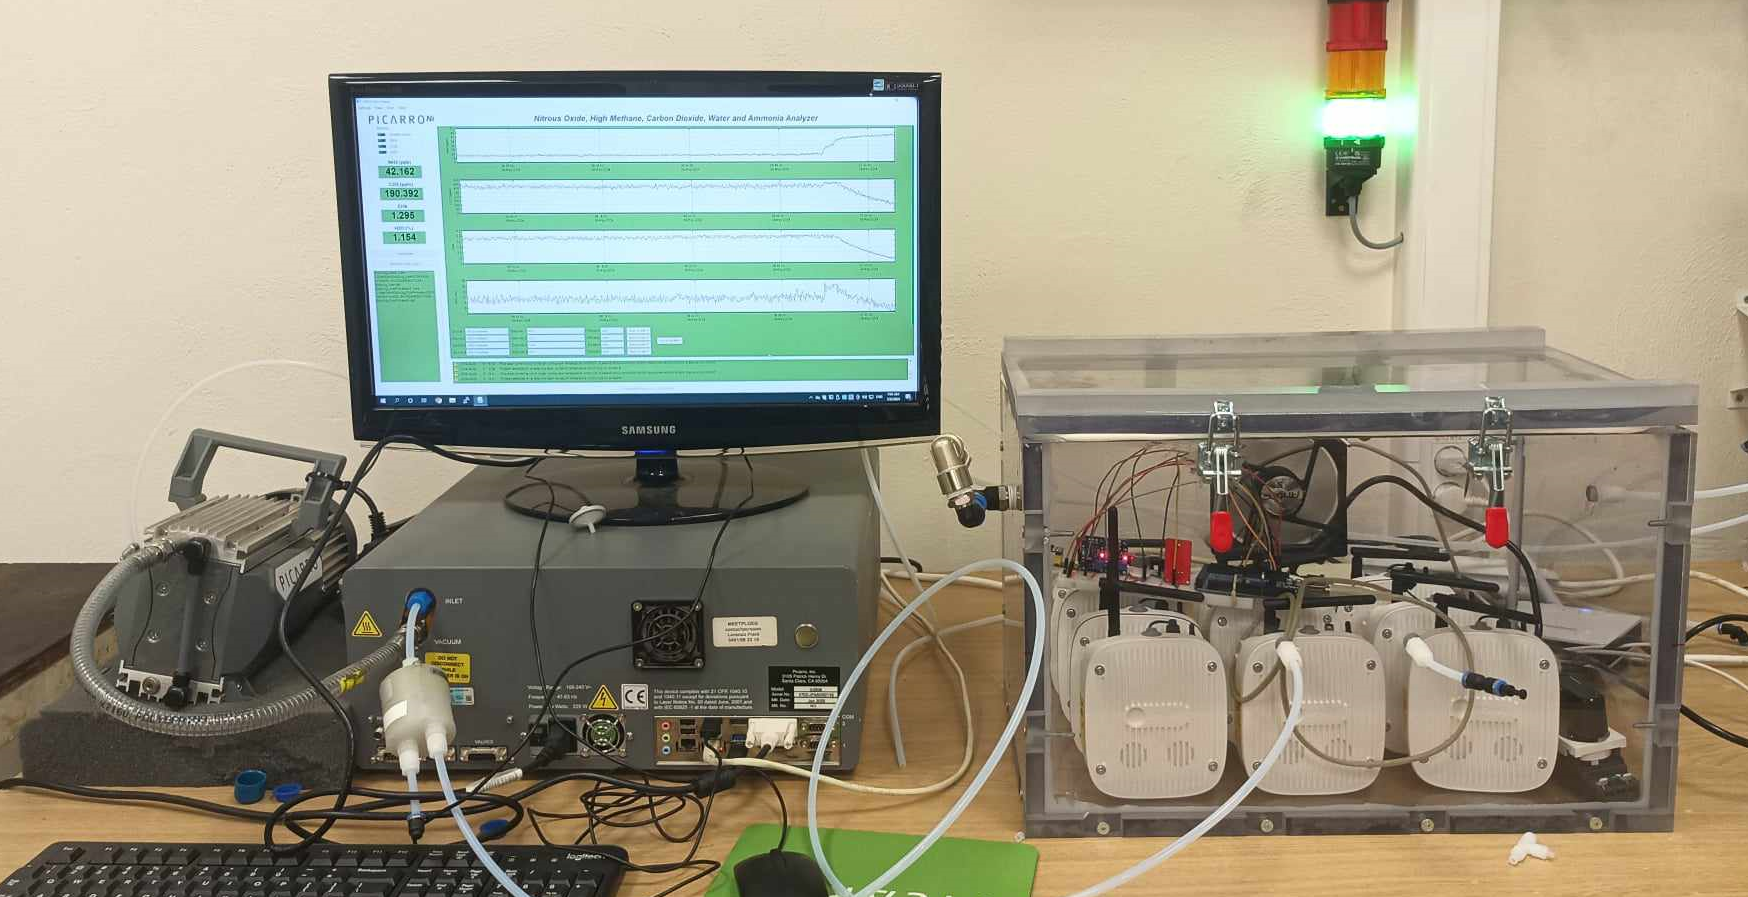
\includegraphics[scale=0.3, center]{test.png}
    \caption[Kalibratiesetup]{De kalibratiesetup bij ILVO met de Picarro gassensor (links) en de luchtdichte kist met de gassensoren (rechts)}
    \label{fig:test}
\end{figure}









\chapter{Analyse van de reslutaten}%
\label{ch:analyse}

\section{Nauwkeurigheid MQ-sensoren}
\label{sec:nauwkeurigheid}

\subsection{Ammoniak (NH\textsubscript{3})}
\label{subsec:nh3}

TODO


\subsection{Koolstofdioxide (CO\textsubscript{2})}
\label{subsec:co2}

TODO (de CO2 test gaat aanstaande woensdag door)

\section{Analyse van de warmte-koelcyclus}
\label{sec:analyse_mq7}

Zoals reeds aangehaald in sectie~\ref{sec:warmte_koel} is de warmte-koelcyclus getest in een normale omgeving, dit was buiten, en een omgeving met een hoge luchtvochtigheid, dit was een dampige badkamer. Zo zijn er per omgeving 3 gassen getest: alcohol, CO en LPG. De resultaten werden in de databank opgeslagen en gevisualiseerd in PowerBI. De resultaten zijn te zien op de volgende figuren, waarbij de blootstelling aan het specifieke gas in het rood staat gekleurd.

\begin{figure}[h!]
    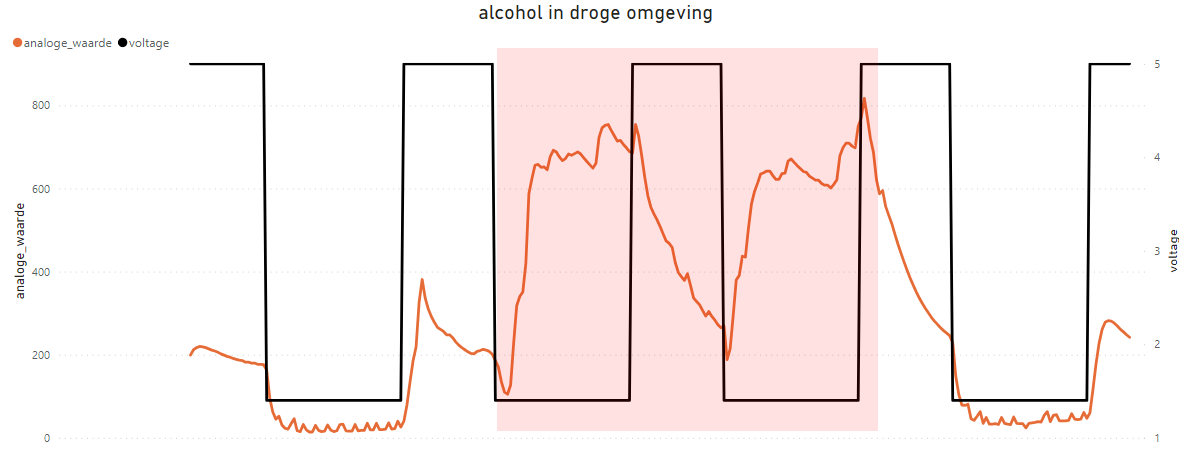
\includegraphics[scale=0.65, center]{alcohol_droog.png}
    \caption[Alcohol in droge omgeving]{Alcohol in droge omgeving}
    \label{fig:alcohol_droog}
\end{figure}

\begin{figure}[h!]
    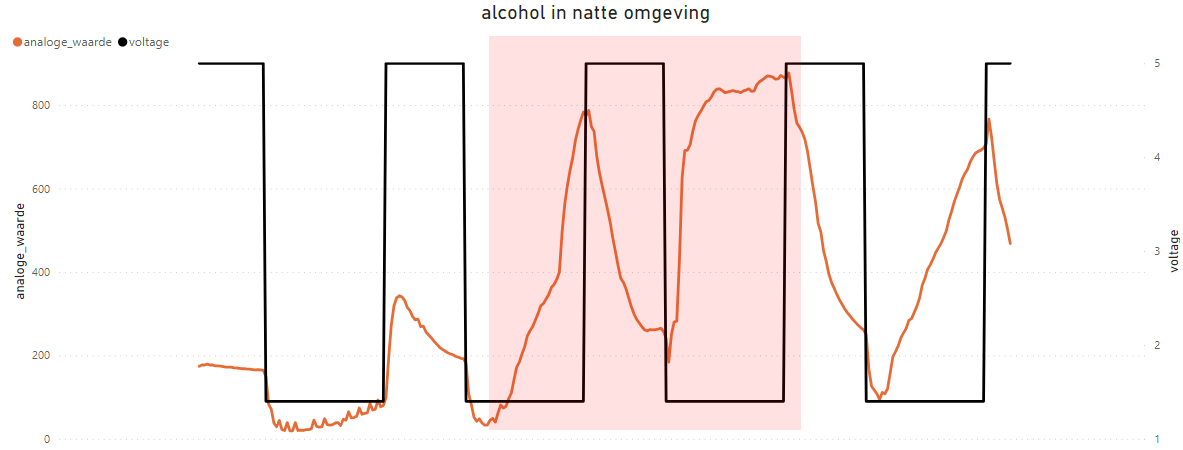
\includegraphics[scale=0.65, center]{alcohol_nat.png}
    \caption[Alcohol in natte omgeving]{Alcohol in natte omgeving}
    \label{fig:alcohol_nat}
\end{figure}

\begin{figure}[h!]
    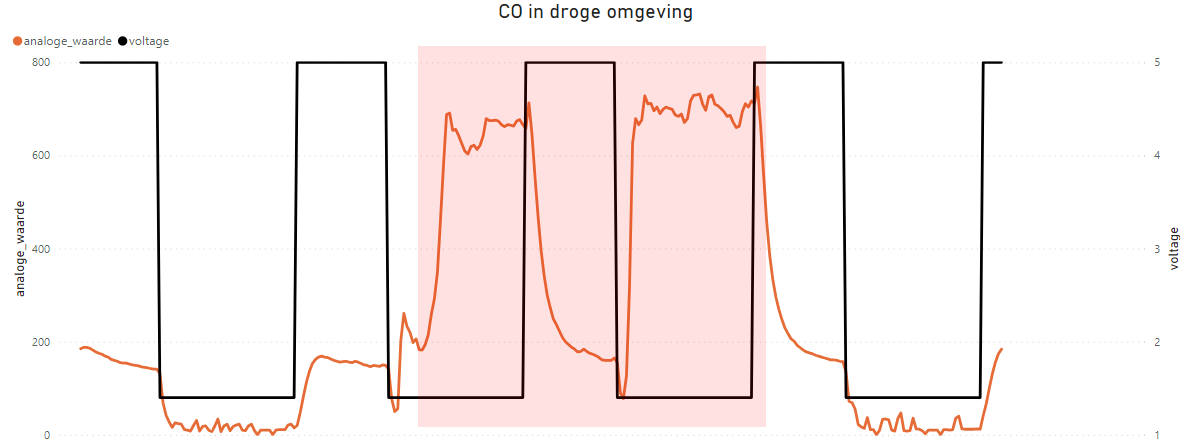
\includegraphics[scale=0.65, center]{co_droog.png}
    \caption[CO in droge omgeving]{CO in droge omgeving}
    \label{fig:co_droog}
\end{figure}

\begin{figure}[h!]
    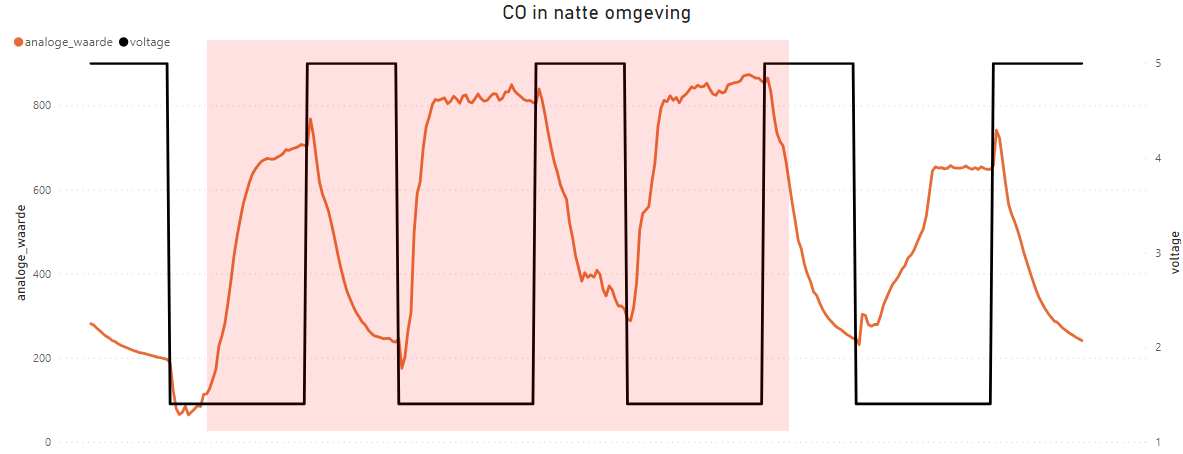
\includegraphics[scale=0.65, center]{co_nat.png}
    \caption[CO in natte omgeving]{CO in natte omgeving}
    \label{fig:co_nat}
\end{figure}

\begin{figure}[h!]
    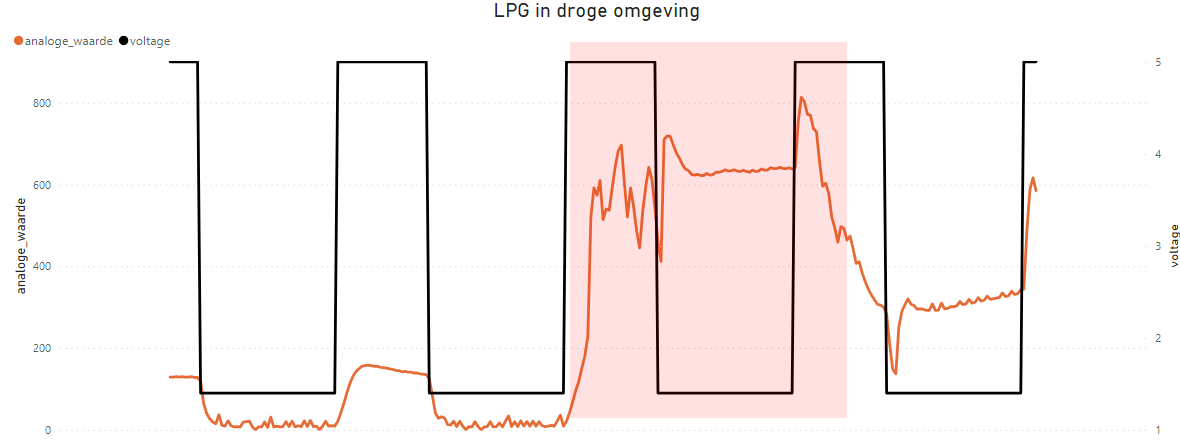
\includegraphics[scale=0.65, center]{lpg_droog.png}
    \caption[LPG in droge omgeving]{LPG in droge omgeving}
    \label{fig:lpg_droog}
\end{figure}

\begin{figure}[h!]
    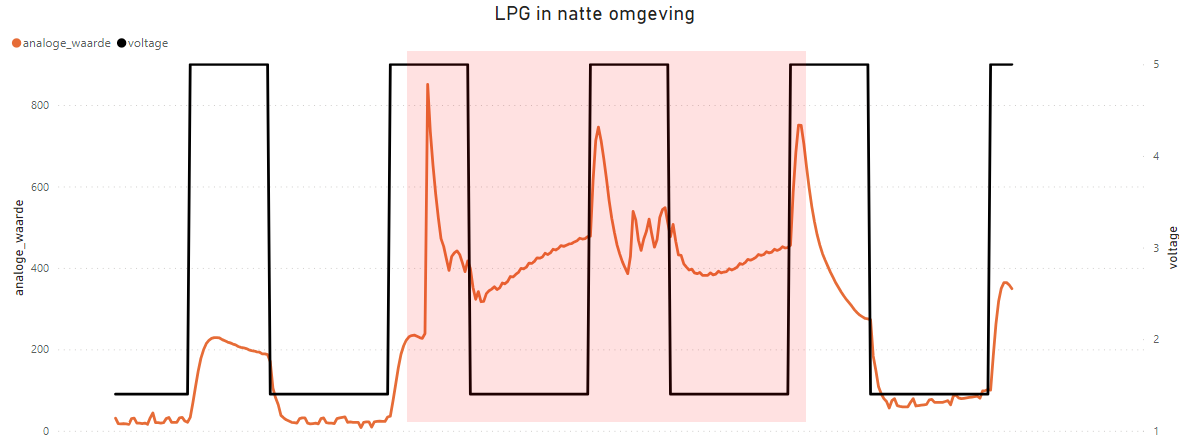
\includegraphics[scale=0.65, center]{lpg_nat.png}
    \caption[LPG in natte omgeving]{LPG in natte omgeving}
    \label{fig:lpg_nat}
\end{figure}


%\pagebreak
\clearpage
\subsection{Invloed van luchtvochtigheid}
\label{subsec:invloed_hum}

Op de resultaten is te zien dat de luchtvochtigheid wel degelijk een rol speelt bij de lezingen van de MQ-7 sensor. 

Het eerste wat opvalt is dat zowel bij alcohol (\ref{fig:alcohol_droog} \&~\ref{fig:alcohol_nat}) als CO (\ref{fig:co_droog} \&~\ref{fig:co_nat}) de waarde hoger is in een vochtige omgeving dan in een normale omgeving, terwijl voor LPG (\ref{fig:lpg_droog} \&~\ref{fig:lpg_nat}) juist het omgekeerde geldt. Dit verschijnsel kan worden verklaart met het feit dat stoffen homo- en heterogeen kunnen zijn.
Door de vochtige omgeving zit de sensor vol met watermoleculen. Doordat water en LPG sterk heterogeen zijn, en dus net als water en olie niet kunnen worden gemengd, zal deze sensor bij aanraking met LPG een minder hoge waarde uitlezen als normaal. Omdat CO juist homogeen is zijn de waarden hier hoger dan normaal. Bij alcohol kan de mengbaarheid afhangen van de soort alcohol, in dit geval is er ontsmettingsalcohol gebruikt die volgens de deze redenering dus ook homogeen blijkt te zijn met water.

Bij zowel alcohol als CO zijn er weinig verschillen in de droge- en natte grafieken, naast dat de waarde hoger wordt dan normaal en iets stabieler is in de koelfase. Maar bij LPG is er een duidelijker verschil te zien in de koelfase. Zo stabiliseert de waarde vrij snel in de droge omgeving (\ref{fig:lpg_droog}), terwijl ze in natte omgeving (\ref{fig:lpg_nat}) juist heel geleidelijk aan toeneemt.


\subsection{Onderscheiden van verschillende gassen}
\label{subsec:onderscheiding_gassen}


Omdat elk soort gas zich anders gedraagt zouden deze onderscheidbaar moeten kunnen zijn op de grafieken. Zo valt meteen de grafiek van CO op (\ref{fig:co_droog}). De MQ-7 sensor is het meest gevoelig voor CO en op de grafiek is dan ook merkbaar hoe snel de waarde klimt wanneer de sensor wordt blootgesteld aan CO. Ook zal de CO het snelste worden weggedreven door een hoge temperatuur.

Alcohol (\ref{fig:alcohol_droog}) klimt daarentegen trager en is veel minder stabiel, waardoor de uiteindelijke lezing na de koelcyclus minder kan accuraat zijn.

LPG heeft de meest merkbare grafiek (\ref{fig:lpg_droog}), zo is te zien hoe LPG zeer stabiel is in de koelcyclus. En tijdens de warmtecyclus een minder grote dip neemt dan de andere gassen. 

Hieruit kan worden opgemerkt dat MQ-7 sensor minder gevoelig is voor alcohol dan LPG en CO. Dit wordt ook aangetoond in de gevoeligheidscurve van de MQ-7 datasheet
%TODO bron datasheet mq7
te zien in figuur~\ref{fig:MQ7_grafiek}.

\begin{figure}[h]
    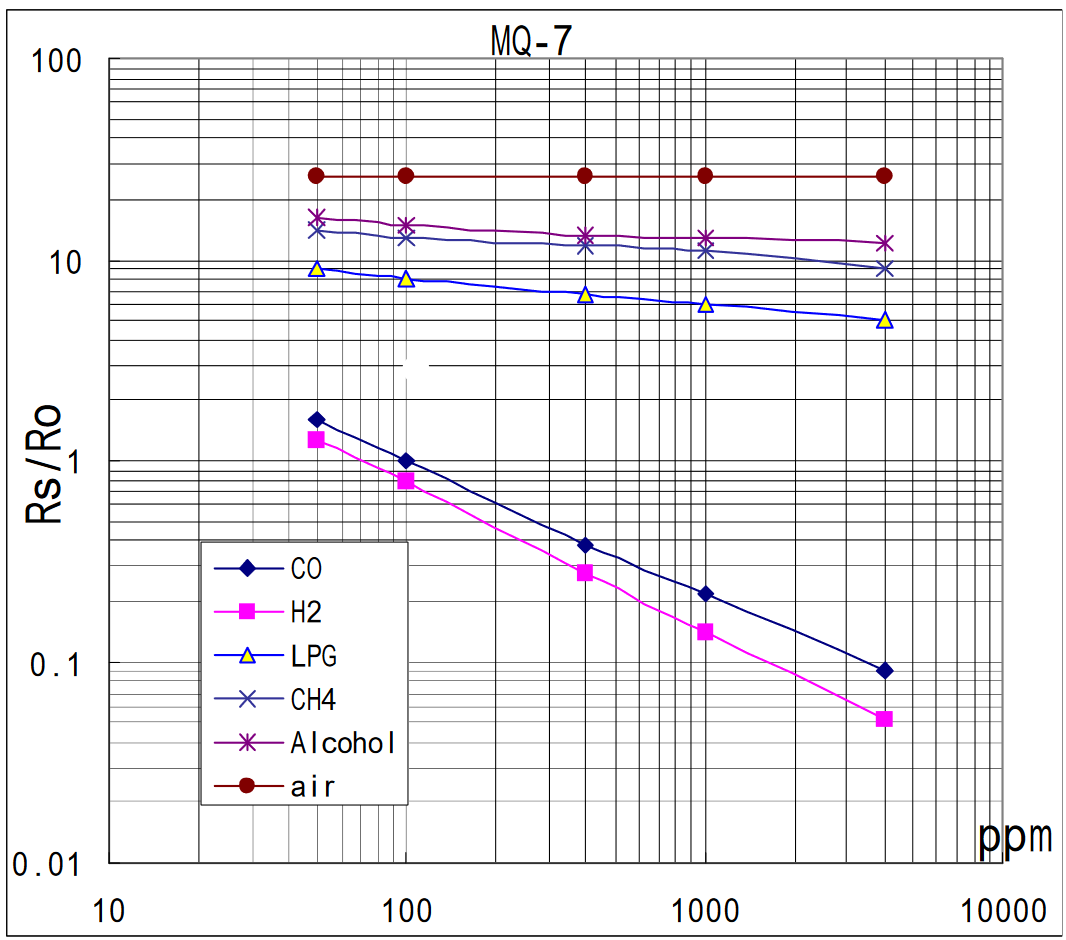
\includegraphics[scale=0.4, center]{MQ7_grafiek.png}
    \caption[Gevoeligheidscurve MQ-7]{Gevoeligheidscurve van de MQ-7 sensor
        %TODO bron datasheet mq135
    }
    \label{fig:MQ7_grafiek}
\end{figure}
















%%=============================================================================
%% Conclusie
%%=============================================================================

\chapter{Conclusie}%
\label{ch:conclusie}

% TODO: Trek een duidelijke conclusie, in de vorm van een antwoord op de
% onderzoeksvra(a)g(en). Wat was jouw bijdrage aan het onderzoeksdomein en
% hoe biedt dit meerwaarde aan het vakgebied/doelgroep? 
% Reflecteer kritisch over het resultaat. In Engelse teksten wordt deze sectie
% ``Discussion'' genoemd. Had je deze uitkomst verwacht? Zijn er zaken die nog
% niet duidelijk zijn?
% Heeft het onderzoek geleid tot nieuwe vragen die uitnodigen tot verder 
%onderzoek?

%centrale onderzoeksvraag: Hoe geschikt zijn goedkope sensoren om gassen in stalomgevingen te meten?
%deelonderzoeksvragen:  - Hoe gaat een MQ-gassensor te werk?
%                       - Hoe kunnen deze gassensoren de luchtsamenstelling meten?
%                       - Zijn deze gassensoren geschikt om de luchtsamenstelling uit te lezen?
%                       - Hoe werkt een warmte-koelcyclus in een sensor en heeft dit voordelen?



In deze studie werd onderzocht hoe geschikt goedkope sensoren zijn om gassen in stalomgeving te meten. De geteste gassensoren zijn de goedkope MQ-sensoren, die kunnen worden bestuurd via een microcontroller zoals Arduino. Er werd onderzocht welke gassen er in een stalomgeving voorkomen en hoe een MQ-sensor exact werkt. Via de informatie uit de datasheets werd berekend hoe deze sensor de luchtsamenstelling kon meten. 
Zo is er tot de conclusie gekomen dat deze MQ-sensoren niet geschikt zijn om de luchtsamenstelling uit te lezen. De MQ-sensoren zijn zeer instabiel en de luchtsamenstelling is een berekende schatting op basis van 1 waarde. 
%TODO Na de R\textsubscript{0}-waarde te berekenen kunnen sommige gassen wel ongeveer correct worden ingeschat, zoals bijvoorbeeld CO\textsubscript{2}, Maar andere gassen worden totaal verkeerd ingeschat. 
Wat deze gassensoren wel kunnen is detecteren of er een te grote hoeveelheid gas aanwezig is, dit kan ze bruikbaar maken als een goedkope monitor die via een alarmsignaal zou kunnen laten weten wanneer de omgeving een te slechte luchtkwaliteit heeft.
Ook bevatten de datasheets niet heel veel informatie waardoor het kalibratieproces moeilijk kan verlopen. 

Hiernaast werd ook de toepassing van een warmte-koelcyclus uitgetest.
%TODO stabieler dan andere?
Het onderscheiden van verschillende gassen via de curve die door deze warmte-koelcyclus wordt gemaakt is iets wat zeker verder onderzocht kan worden. Aangezien elk gas zich op een andere manier gedraagt en TODO








%---------- Bijlagen -----------------------------------------------------------

\appendix

\chapter{Onderzoeksvoorstel}

Het onderwerp van deze bachelorproef is gebaseerd op een onderzoeksvoorstel dat vooraf werd beoordeeld door de promotor. Dat voorstel is opgenomen in deze bijlage.


\section*{Samenvatting}

    Dit onderzoek richt zich op het ontwikkelen en evalueren van goedkope gassensoren, met name MQ-sensoren, die via breakout boards de luchtkwaliteit in varkensstallen kunnen meten. De motivatie voor dit onderzoek ligt in de problematiek van schadelijke stalgassen die een bedreiging vormen voor zowel dieren als mensen, alsook voor de biodiversiteit in de omgeving van de stal. Omdat professionele gassensoren zeer duur zijn en niet thuishoren in een stalomgeving, zou deze studie als inspiratie kunnen dienen voor onderzoekers en fabrikanten van gassensoren, om nieuwe producten te maken die geschikt zijn om in een stalomgeving te werken. De methodologie omvat een literatuurstudie, de bouw en programmering van de sensor en databank, experimenten zowel binnen- als buitenshuis, en een analyse van de verzamelde gegevens. Uit dit onderzoek zou een breakoutboard met meerdere gassensoren komen die in staat is de luchtkwaliteit van een stal te bepalen.
    
    

% Kopieer en plak hier de samenvatting (abstract) van je onderzoeksvoorstel.

% Verwijzing naar het bestand met de inhoud van het onderzoeksvoorstel
%---------- Inleiding ---------------------------------------------------------


%TODO
% -kost NodeMCU geld?
% -thingsboard API
% -mail sturen pieterjan
% -mail promotor


\section{Introductie}%
\label{sec:introductie}

\begin{comment}

Waarover zal je bachelorproef gaan? Introduceer het thema en zorg dat volgende zaken zeker duidelijk aanwezig zijn:

\begin{itemize}
  \item kaderen thema
  \item de doelgroep -> varkenshouders
  \item de probleemstelling en (centrale) onderzoeksvraag
  \item de onderzoeksdoelstelling
\end{itemize}

Denk er aan: een typische bachelorproef is \textit{toegepast onderzoek}, wat betekent dat je start vanuit een concrete probleemsituatie in bedrijfscontext, een \textbf{casus}. Het is belangrijk om je onderwerp goed af te bakenen: je gaat voor die \textit{ene specifieke probleemsituatie} op zoek naar een goede oplossing, op basis van de huidige kennis in het vakgebied.

De doelgroep moet ook concreet en duidelijk zijn, dus geen algemene of vaag gedefinieerde groepen zoals \emph{bedrijven}, \emph{developers}, \emph{Vlamingen}, enz. Je richt je in elk geval op it-professionals, een bachelorproef is geen populariserende tekst. Eén specifiek bedrijf (die te maken hebben met een concrete probleemsituatie) is dus beter dan \emph{bedrijven} in het algemeen.

Formuleer duidelijk de onderzoeksvraag! De begeleiders lezen nog steeds te veel voorstellen waarin we geen onderzoeksvraag terugvinden.

Schrijf ook iets over de doelstelling. Wat zie je als het concrete eindresultaat van je onderzoek, naast de uitgeschreven scriptie? Is het een proof-of-concept, een rapport met aanbevelingen, \ldots Met welk eindresultaat kan je je bachelorproef als een succes beschouwen?

\end{comment}


Elk jaar gaan er duizenden varkens dood aan vergiftiging door schadelijke stalgassen \autocite{Sercu2023}, gassen zoals koolstofmonoxide (CO), koolstofdioxide (CO\textsubscript{2}), ammoniak (NH\textsubscript{3}) en methaan (CH\textsubscript{4}) ontstaan in de mest van varkens door de afbraak van aanwezige eiwitten door bacteriën \autocite{Wolf2013}. Deze gassen kunnen bij ophoping zeer giftig zijn voor zowel de dieren als voor mensen. Ook kan er door deze gassen een afname van biodiversiteit in de directe omgeving van de stal ontstaan. Dat komt voornamelijk door ammoniak, ammoniak zorgt voor vermesting waardoor de grond steeds rijker wordt aan voedingsstoffen. Hierdoor worden veel planten verdrongen door planten zoals gras en brandnetels, dit zorgt voor minder planten en dieren waardoor de biodiversiteit verslechtert. Ook kan er in de buurt van een varkensstal last van geurhinder zijn door de grote hoeveelheid ammoniak in de lucht \autocite{RSS2020}.

Het monitoren van het stalklimaat kan door verschillende gassensoren worden gedaan, maar een professionele sensor kan al snel zeer duur zijn. Deze gassensoren zijn bovendien meestal niet gemaakt voor een stalomgeving, wat hun levensduur sterk kan verminderen. Daarom luidt de centrale onderzoeksvraag als volgt: ''Hoe geschikt zijn goedkope sensoren om gassen in stalomgevingen te meten?''. Het onderzoek zal zich richten op goedkope gassensoren die aan de hand van breakout boards de luchtkwaliteit van een stal kunnen bepalen. Er zal aandacht worden besteed aan hoe deze sensoren in precies elkaar zitten, hun nauwkeurigheid en geschiktheid voor gebruik in stalomgevingen, en hoe de bekomen data kan worden opgeslagen en geïnterpreteerd.

De doelgroep voor deze studie zijn fabrikanten van gassensoren, dit onderzoek kan als inspiratie dienen om nieuwe producten te ontwikkelen speciaal voor veehouders. De onderzoekers van deze fabrikanten zouden deze studie kunnen gebruiken om op een goedkope manier een test set-up van een gassensor in elkaar te zetten. Deze test-setup zou dan uiteindelijk kunnen dienen tot een professionele gassensor, die geschikt is om in een stalomgeving de luchtkwaliteit te monitoren. Hierdoor zullen veehouders sneller gemotiveerd zijn om gassensoren te implementeren die voldoende geschikt zijn voor een stalomgeving, omdat ze verantwoordelijk zijn voor het verbeteren van de gezondheid van hun dieren en de omgeving.


%---------- Stand van zaken ---------------------------------------------------


\section{State-of-the-art}%
\label{sec:state-of-the-art}

\begin{comment}

Hier beschrijf je de \emph{state-of-the-art} rondom je gekozen onderzoeksdomein, d.w.z.\ een inleidende, doorlopende tekst over het onderzoeksdomein van je bachelorproef. Je steunt daarbij heel sterk op de professionele \emph{vakliteratuur}, en niet zozeer op populariserende teksten voor een breed publiek. Wat is de huidige stand van zaken in dit domein, en wat zijn nog eventuele open vragen (die misschien de aanleiding waren tot je onderzoeksvraag!)?

Je mag de titel van deze sectie ook aanpassen (literatuurstudie, stand van zaken, enz.). Zijn er al gelijkaardige onderzoeken gevoerd? Wat concluderen ze? Wat is het verschil met jouw onderzoek?

Verwijs bij elke introductie van een term of bewering over het domein naar de vakliteratuur, bijvoorbeeld~\autocite{Hykes2013}! Denk zeker goed na welke werken je refereert en waarom.

Draag zorg voor correcte literatuurverwijzingen! Een bronvermelding hoort thuis \emph{binnen} de zin waar je je op die bron baseert, dus niet er buiten! Maak meteen een verwijzing als je gebruik maakt van een bron. Doe dit dus \emph{niet} aan het einde van een lange paragraaf. Baseer nooit teveel aansluitende tekst op eenzelfde bron.

Als je informatie over bronnen verzamelt in JabRef, zorg er dan voor dat alle nodige info aanwezig is om de bron terug te vinden (zoals uitvoerig besproken in de lessen Research Methods).

% Voor literatuurverwijzingen zijn er twee belangrijke commando's:
% \autocite{KEY} => (Auteur, jaartal) Gebruik dit als de naam van de auteur
%   geen onderdeel is van de zin.
% \textcite{KEY} => Auteur (jaartal)  Gebruik dit als de auteursnaam wel een
%   functie heeft in de zin (bv. ``Uit onderzoek door Doll \& Hill (1954) bleek
%   ...'')

Je mag deze sectie nog verder onderverdelen in subsecties als dit de structuur van de tekst kan verduidelijken.



%------------------------------------------------------------------------------

-welke gassen zijn schadelijk voor varkens?
-wat is de normale concentratie van deze gassen?
-welke soort sensoren zijn er?
-hoe worden gassen gemeten met deze sensoren?
\end{comment}

Volgens \textcite{Klooster1993} zijn de meest voorkomende stalgassen in een varkensstal ammoniak, koolstofdioxide, zuurstof en waterdamp. Ammoniak is een afbraakproduct van eiwitten in de voeding en de mest \autocite{Wolf2013}. Al vanaf 20 ppm in de lucht treden er schadelijke effecten bij varkens, daarom ligt de ArBO-norm op 10 ppm. Koolstofdioxide wordt door varkens en mensen zelf geproduceerd, en bij onvoldoende ventilatie kan de concentratie CO\textsubscript{2} zo hoog oplopen dat er verstikking optreedt. Dit kan gebeuren bij concentraties van meer dan 40 volumeprocenten, de Aronorm ligt op 0,35 tot 0,5 volumeprocent maar er wordt gestreefd naar concentraties tussen de 0,2 en 0,3 volumeprocent.

Een populaire en goedkope manier om gasconcentraties te meten is door het gebruik van MQ-sensoren \autocite{Khadim2021}, deze gassensoren kosten rond de 5 euro en kunnen veel verschillende gasconcentraties meten, via een arduino kan deze data dan worden verwerkt. Deze sensoren bestaan uit een elektrode waarop een sensorsubstantie is geplaatst en die wordt verwarmd om de reactiviteit en gevoeligheid te vergroten. Wanneer er een bepaald type gas passeert veranderd de weerstand van deze elektrode, hierdoor kan er worden gemeten in welke hoeveelheid een bepaald type gas voorkomt \autocite{RC2022}. Er zijn veel verschillende soorten MQ-sensoren, de sensoren die het meest geschikt lijken voor dit onderzoek zijn de MQ-4, MQ-7 en MQ-135 sensoren. Methaan kan worden gemeten met de MQ-4, koolstofmonoxide met de MQ-7 en de MQ-135 is gespecialiseerd in het meten van de luchtkwaliteit (met name koolstof, ammoniak, benzeen, alcohol en rook). Door verschillende sensoren te testen kunnen deze worden vergeleken en gecombineerd \autocite{Soloupis2022}.


Om de resultaten in realtime af te kunnen lezen kan er gebruik worden gemaakt van een LCD display, maar het toevoegen van een display verhoogt de kosten en het energieverbruik. Daarom zal er een web-based user interface worden gemaakt, dit kan worden gedaan met verschillende tools. Via Involt bijvoorbeeld, een framework waarmee er via html en css een gui kan worden gemaakt die met arduino werkt \autocite{Involt}. Ook kan er een systeem worden gemaakt zoals in de studie van \textcite{Rani2020}, waar de arduino via een ESP8266 Wi-Fi module de data naar een Thingsboard server pusht via een MQTT protocol (Message Queuing Telemetry Transport).

%Ook kan er gebruik worden gemaakt van een systeem zoals in de studie van \textcite{Chanthakit2018}, waar een NodeMCU de gegevens van de sensoren verzamelt en ze doorgeeft aan MQTT die berichten stuurt naar de Node-RED tool die op zijn beurt de gegevens plaatst op een dashboard.

Het meten van gassen door MQ-sensoren is al veel onderzocht, maar nog niet in verband met varkensstallen. Onderzoeken zoals die van \textcite{Gorakhpur2020} tonen hoe een MQ-135 sensor kan worden gebruikt met behulp van Arduino. Het onderzoek van \textcite{Vijayalakshmi2019} toont aan dat een MQ-135 sensor kan worden gebruikt om grote hoeveelheden ammoniakgas in laboratoria, industrieën en fabrieken te detecteren. Hier worden er ook waarschuwingen verstuurd via het IoT device. 




%---------- Methodologie ------------------------------------------------------
\section{Methodologie}%
\label{sec:methodologie}

\begin{comment}

Hier beschrijf je hoe je van plan bent het onderzoek te voeren. Welke onderzoekstechniek ga je toepassen om elk van je onderzoeksvragen te beantwoorden? Gebruik je hiervoor literatuurstudie, interviews met belanghebbenden (bv.~voor requirements-analyse), experimenten, simulaties, vergelijkende studie, risico-analyse, PoC, \ldots?

Valt je onderwerp onder één van de typische soorten bachelorproeven die besproken zijn in de lessen Research Methods (bv.\ vergelijkende studie of risico-analyse)? Zorg er dan ook voor dat we duidelijk de verschillende stappen terug vinden die we verwachten in dit soort onderzoek!

Vermijd onderzoekstechnieken die geen objectieve, meetbare resultaten kunnen opleveren. Enquêtes, bijvoorbeeld, zijn voor een bachelorproef informatica meestal \textbf{niet geschikt}. De antwoorden zijn eerder meningen dan feiten en in de praktijk blijkt het ook bijzonder moeilijk om voldoende respondenten te vinden. Studenten die een enquête willen voeren, hebben meestal ook geen goede definitie van de populatie, waardoor ook niet kan aangetoond worden dat eventuele resultaten representatief zijn.

Uit dit onderdeel moet duidelijk naar voor komen dat je bachelorproef ook technisch voldoen\-de diepgang zal bevatten. Het zou niet kloppen als een bachelorproef informatica ook door bv.\ een student marketing zou kunnen uitgevoerd worden.

Je beschrijft ook al welke tools (hardware, software, diensten, \ldots) je denkt hiervoor te gebruiken of te ontwikkelen.

Probeer ook een tijdschatting te maken. Hoe lang zal je met elke fase van je onderzoek bezig zijn en wat zijn de concrete \emph{deliverables} in elke fase?

\end{comment}


%------------------------------------------------------------------------------


Het onderzoek zal worden gevoerd met verschillende onderzoekstechnieken, waaronder als eerste een grondige literatuurstudie. In deze literatuurstudie zullen verschillende zaken worden onderzocht zoals wat normale gasconcentraties zijn in een stal, welke schadelijke gassen er allemaal zijn, welk effect deze hebben en hoe deze kunnen worden gemeten. Ook zal de werking van MQ sensoren in detail worden onderzocht om te begrijpen hoe deze juist te werk gaan.

%Hierna zal het breakoutboard met de sensoren daadwerkelijk in elkaar worden gestoken en zal de software worden geprogrammeerd. Er zal een user interface worden gemaakt die het gemakkelijk maakt om alle resultaten in af te lezen, en ook wordt een databank opgesteld waar op ieder bepaald tijdsinterval de gasconcentratie zal worden opgeslagen. Hierna gaan de experimenten aan de slag, eerst zal er worden nagegaan of wat de sensoren meten wel degelijk kan worden gebruikt om de luchtkwaliteit te monitoren. Op basis hiervan wordt beoordeeld of er aanpassingen nodig zijn aan een sensor, en indien van toepassing, welke specifieke aanpassingen noodzakelijk zijn. Vervolgens zullen de sensoren binnen- en buitenshuis worden getest, dit kan bijvoorbeeld ook door op de sensor te ademen en te kijken of er een verhoging in CO\textsubscript{2} is. Ook kan de gassensor daadwerkelijk in een stalomgeving worden geëvalueerd. Omdat ILVO beschikt over een dure en professionele gassensor kunnen hiermee dezelfde experimenten mee worden gedaan, om zo de nauwkeurigheid te bepalen van de MQ sensoren. Nadien zal het monitoren van deze concentraties gedurende een tijdspanne worden getest. Ten slotte zullen deze gegevens worden gevisualiseerd in PowerBI waardoor er conclusies zullen kunnen worden getrokken.

Hierna zal het breakoutboard met de sensoren daadwerkelijk in elkaar worden gestoken en zal de software worden geprogrammeerd. Er zal een user interface worden gemaakt die het gemakkelijk maakt om alle resultaten in af te lezen, en ook wordt een databank opgesteld waar op ieder bepaald tijdsinterval de gasconcentratie zal worden opgeslagen. Hierna gaan de experimenten aan de slag, eerst zal er worden nagegaan of wat de sensoren meten wel degelijk kan worden gebruikt om de luchtkwaliteit te monitoren. Op basis hiervan wordt beoordeeld of er aanpassingen nodig zijn aan een sensor, en indien van toepassing, welke specifieke aanpassingen noodzakelijk zijn. Vervolgens zullen de sensoren binnen- en buitenshuis worden getest, dit kan bijvoorbeeld ook door op de sensor te ademen en te kijken of er een verhoging in CO\textsubscript{2} is. Ook kan de gassensor daadwerkelijk in een stalomgeving worden geëvalueerd. Nadien zal het monitoren van deze concentraties gedurende een tijdspanne worden getest. Ten slotte zullen deze gegevens worden gevisualiseerd in PowerBI waardoor er conclusies zullen kunnen worden getrokken.

Er zullen verschillende tools voor dit onderzoek worden gebruikt. MQ-sensoren, een arduino uno en een breakout board met de nodige hardware zijn de basis tools. Hiernaast is er ook nog de Arduino IDE nodig voor het programmeren van de sensor en een tool om een user interface te maken. Ook zal er een databank nodig zijn voor de waarden van de gasconcentraties in op te slaan. De analyse en visualisatie van deze gegevens kan worden gedaan met PowerBI.

Dit onderzoek zal in het tweede semester worden uitgevoerd, dat in totaal ongeveer 14 weken is. In de eerste 4 weken zal de literatuurstudie worden uitgevoerd en zal de methodologie worden opgesteld. Hierdoor zal er genoeg kennis zijn verworven om te beginnen met het bouwen en programmeren van de sensor, hiervoor schat ik een 3-tal weken in. In de volgende 4 weken zal er worden geëxperimenteerd met de gassensor, er zal veel data worden verzameld die wordt geanalyseerd in de volgende stap. Voor het opstellen van de conclusie en het vergelijken van deze gemeten resultaten worden 3 weken gerekend.




%---------- Verwachte resultaten ----------------------------------------------
\section{Verwacht resultaat, conclusie}%
\label{sec:verwachte_resultaten}
\begin{comment}
Hier beschrijf je welke resultaten je verwacht. Als je metingen en simulaties uitvoert, kan je hier al mock-ups maken van de grafieken samen met de verwachte conclusies. Benoem zeker al je assen en de onderdelen van de grafiek die je gaat gebruiken. Dit zorgt ervoor dat je concreet weet welk soort data je moet verzamelen en hoe je die moet meten.

Wat heeft de doelgroep van je onderzoek aan het resultaat? Op welke manier zorgt jouw bachelorproef voor een meerwaarde?

Hier beschrijf je wat je verwacht uit je onderzoek, met de motivatie waarom. Het is \textbf{niet} erg indien uit je onderzoek andere resultaten en conclusies vloeien dan dat je hier beschrijft: het is dan juist interessant om te onderzoeken waarom jouw hypothesen niet overeenkomen met de resultaten.


\end{comment}


%------------------------------------------------------------------------------


Als resultaat verwacht ik een proefopstelling van een breakoutboard met meerdere gassensoren die in staat zijn om de concentraties van methaan, koolstofmonoxide, koolstofdioxide en ammoniak op te meten in een stalomgeving. Ik verwacht niet dat deze even accuraat zal zijn als een professionele gassensor, maar wel dat deze op tijd een signaal kan sturen als de gasconcentraties een bepaald limiet hebben overschreven. Verder zal de waarde ieder moment kunnen worden opgevraagd via een user interface, en zal er per bepaald tijdsinterval data worden opgeslagen in de databank. Deze data zou hierna gevisualiseerd kunnen worden door PowerBi, hiermee zullen grafieken mee kunnen worden gemaakt zoals bijvoorbeeld die in figuur 1.

De doelgroep kan met deze studie informatie vergaren over gassensoren die geschikt zijn om in een stalomgeving te hangen. Deze studie zal ook in detail aantonen hoe er zelf een proefopstelling in elkaar kan worden gezet. Het uiteindelijke onderzoek kan vooral als inspiratie dienen voor fabrikanten van gassensoren om nieuwe producten te ontwikkelen voor veehouders.


\begin{figure}
    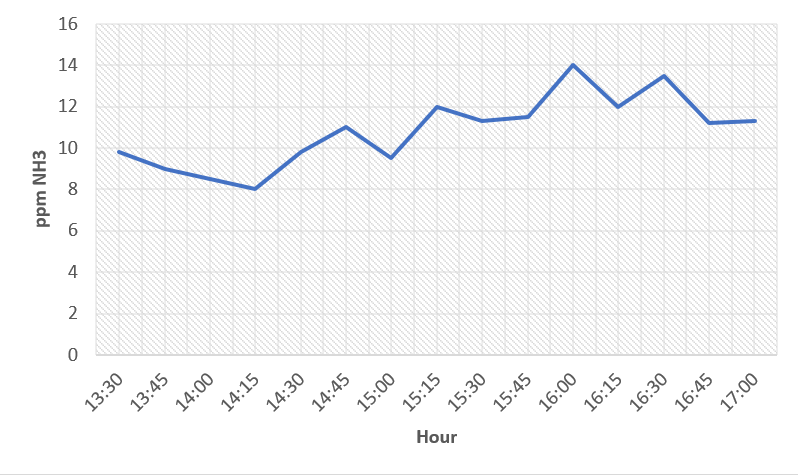
\includegraphics[width=\columnwidth]{mockup grafiek}
    \caption{Voorbeeld grafiek}
\end{figure}








%%---------- Andere bijlagen --------------------------------------------------
% Voeg hier eventuele andere bijlagen toe. Bv. als je deze BP voor de
% tweede keer indient, een overzicht van de verbeteringen t.o.v. het origineel.
\chapter{Bijlage}
%%=============================================================================
%% Voorwoord
%%=============================================================================

\chapter*{Bijlage}%
\label{ch:bijlage}

\section{Berekenen van de R0 waarden}
\label{lst:kalibratie}
\begin{lstlisting}[language=Java, caption={Berekenen van de R0 waarden}]
float R0_berekenen(float analogeWaarde, float luchtconstante) {
    float Rs;
    float R0;
    float V_out;
    float V_cc = 5.0;
    float maxAnaloog = 1023.0;
    float R_l = 1.0;
    
    //waarde omzetten naar spanning
    V_out = (analogeWaarde*V_cc)/maxAnaloog;
    
    //Rs berekenen
    Rs = ((V_cc*R_l)/V_out)-R_l;
    
    //R0 berekenen met luchtconstante
    R0 = Rs/luchtconstante;
    
    return R0;
}
\end{lstlisting}


\section{Berekenen van de ppm waarden voor de MQ-135}
\label{lst:ppm_mq135}
\begin{lstlisting}[language=Java, caption={Berekenen van de ppm waarden voor de MQ-135}]
// ppm meten MQ-135

//R0 berekent met kalibratie script
float R0_MQ135 = 9.59;

float Rs_MQ135;

//pin vd sensor 
int MQ135 = A1;

float analogeWaarde_MQ135;

float MQ135_CO_ppm;
float MQ135_NH4_ppm;
float MQ135_CO2_ppm;
float MQ135_alcohol_ppm;
float MQ135_tolueen_ppm;
float MQ135_aceton_ppm;

//waarden van grafieken (x1, y1, x2, y2)
float MQ135_CO2[4] = {10.72, 2.78, 191.15, 1.35};
float MQ135_NH4[4] = {10.61, 2.49, 190.20, 0.77};
float MQ135_CO[4] = {10.72, 2.24, 188.31, 0.81};
float MQ135_alcohol[4] = {10.51, 1.86, 189.25, 0.74};
float MQ135_tolueen[4] = {10.45, 1.52, 188.31, 0.65};
float MQ135_aceton[4] = {10.72, 1.39, 189.25, 0.59};


void setup() {
    Serial.begin(9600);
}

void loop() {
    analogeWaarde_MQ135 = analogRead(MQ135);
    
    Rs_MQ135 = Rs_berekenen(analogeWaarde_MQ135);
    
    MQ135_CO_ppm = ppm_berekenen(R0_MQ135, Rs_MQ135, MQ135_CO);
    MQ135_NH4_ppm = ppm_berekenen(R0_MQ135, Rs_MQ135, MQ135_NH4);
    MQ135_CO2_ppm = ppm_berekenen(R0_MQ135, Rs_MQ135, MQ135_CO2);
    MQ135_alcohol_ppm = ppm_berekenen(R0_MQ135, Rs_MQ135, MQ135_alcohol);
    MQ135_tolueen_ppm = ppm_berekenen(R0_MQ135, Rs_MQ135, MQ135_tolueen);
    MQ135_aceton_ppm = ppm_berekenen(R0_MQ135, Rs_MQ135, MQ135_aceton);
    
    Serial.print("MQ135_CO_ppm = ");
    Serial.println(MQ135_CO_ppm);
    
    Serial.print("MQ135_NH4_ppm = ");
    Serial.println(MQ135_NH4_ppm);
    
    Serial.print("MQ135_CO2_ppm = ");
    Serial.println(MQ135_CO2_ppm);
    
    Serial.print("MQ135_alcohol_ppm = ");
    Serial.println(MQ135_alcohol_ppm);
    
    Serial.print("MQ135_tolueen_ppm = ");
    Serial.println(MQ135_tolueen_ppm);
    
    Serial.print("MQ135_aceton_ppm = ");
    Serial.println(MQ135_aceton_ppm);
    
    delay(5000);
}


float Rs_berekenen(float analogeWaarde) {
    float Rs;
    float V_out;
    float V_cc = 5.0;
    float maxAnaloog = 1023.0;
    float R_l = 1.0;
    
    //waarde omzetten naar spanning
    V_out = (analogeWaarde*V_cc)/maxAnaloog;
    
    //Rs berekenen
    Rs = ((V_cc*R_l)/V_out)-R_l;
    
    return Rs;
}

float ppm_berekenen(float R0, float Rs, float waarden[4]) {
    float b;
    float m;
    float ppm;
    
    m = (log10(waarden[3])-log10(waarden[1]))/(log10(waarden[2])-log10(waarden[0]));
    b = log10(waarden[1]) - m*log10(waarden[0]);
    
    ppm = pow((Rs/(R0*pow(10, b))),(1/m));
    
    return ppm;
}
    
\end{lstlisting}



\section{Het initialiseren van de ESP01 WiFi module}
\label{sec:esp_init}

\subsection{Downloaden van de firmware}
\label{subsec:firmware}

Figuur \ref{fig:esp_circuit} toont aan hoe de ESP01 moet worden aangesloten om de firmware te kunnen downloaden.

\begin{figure}[h]
    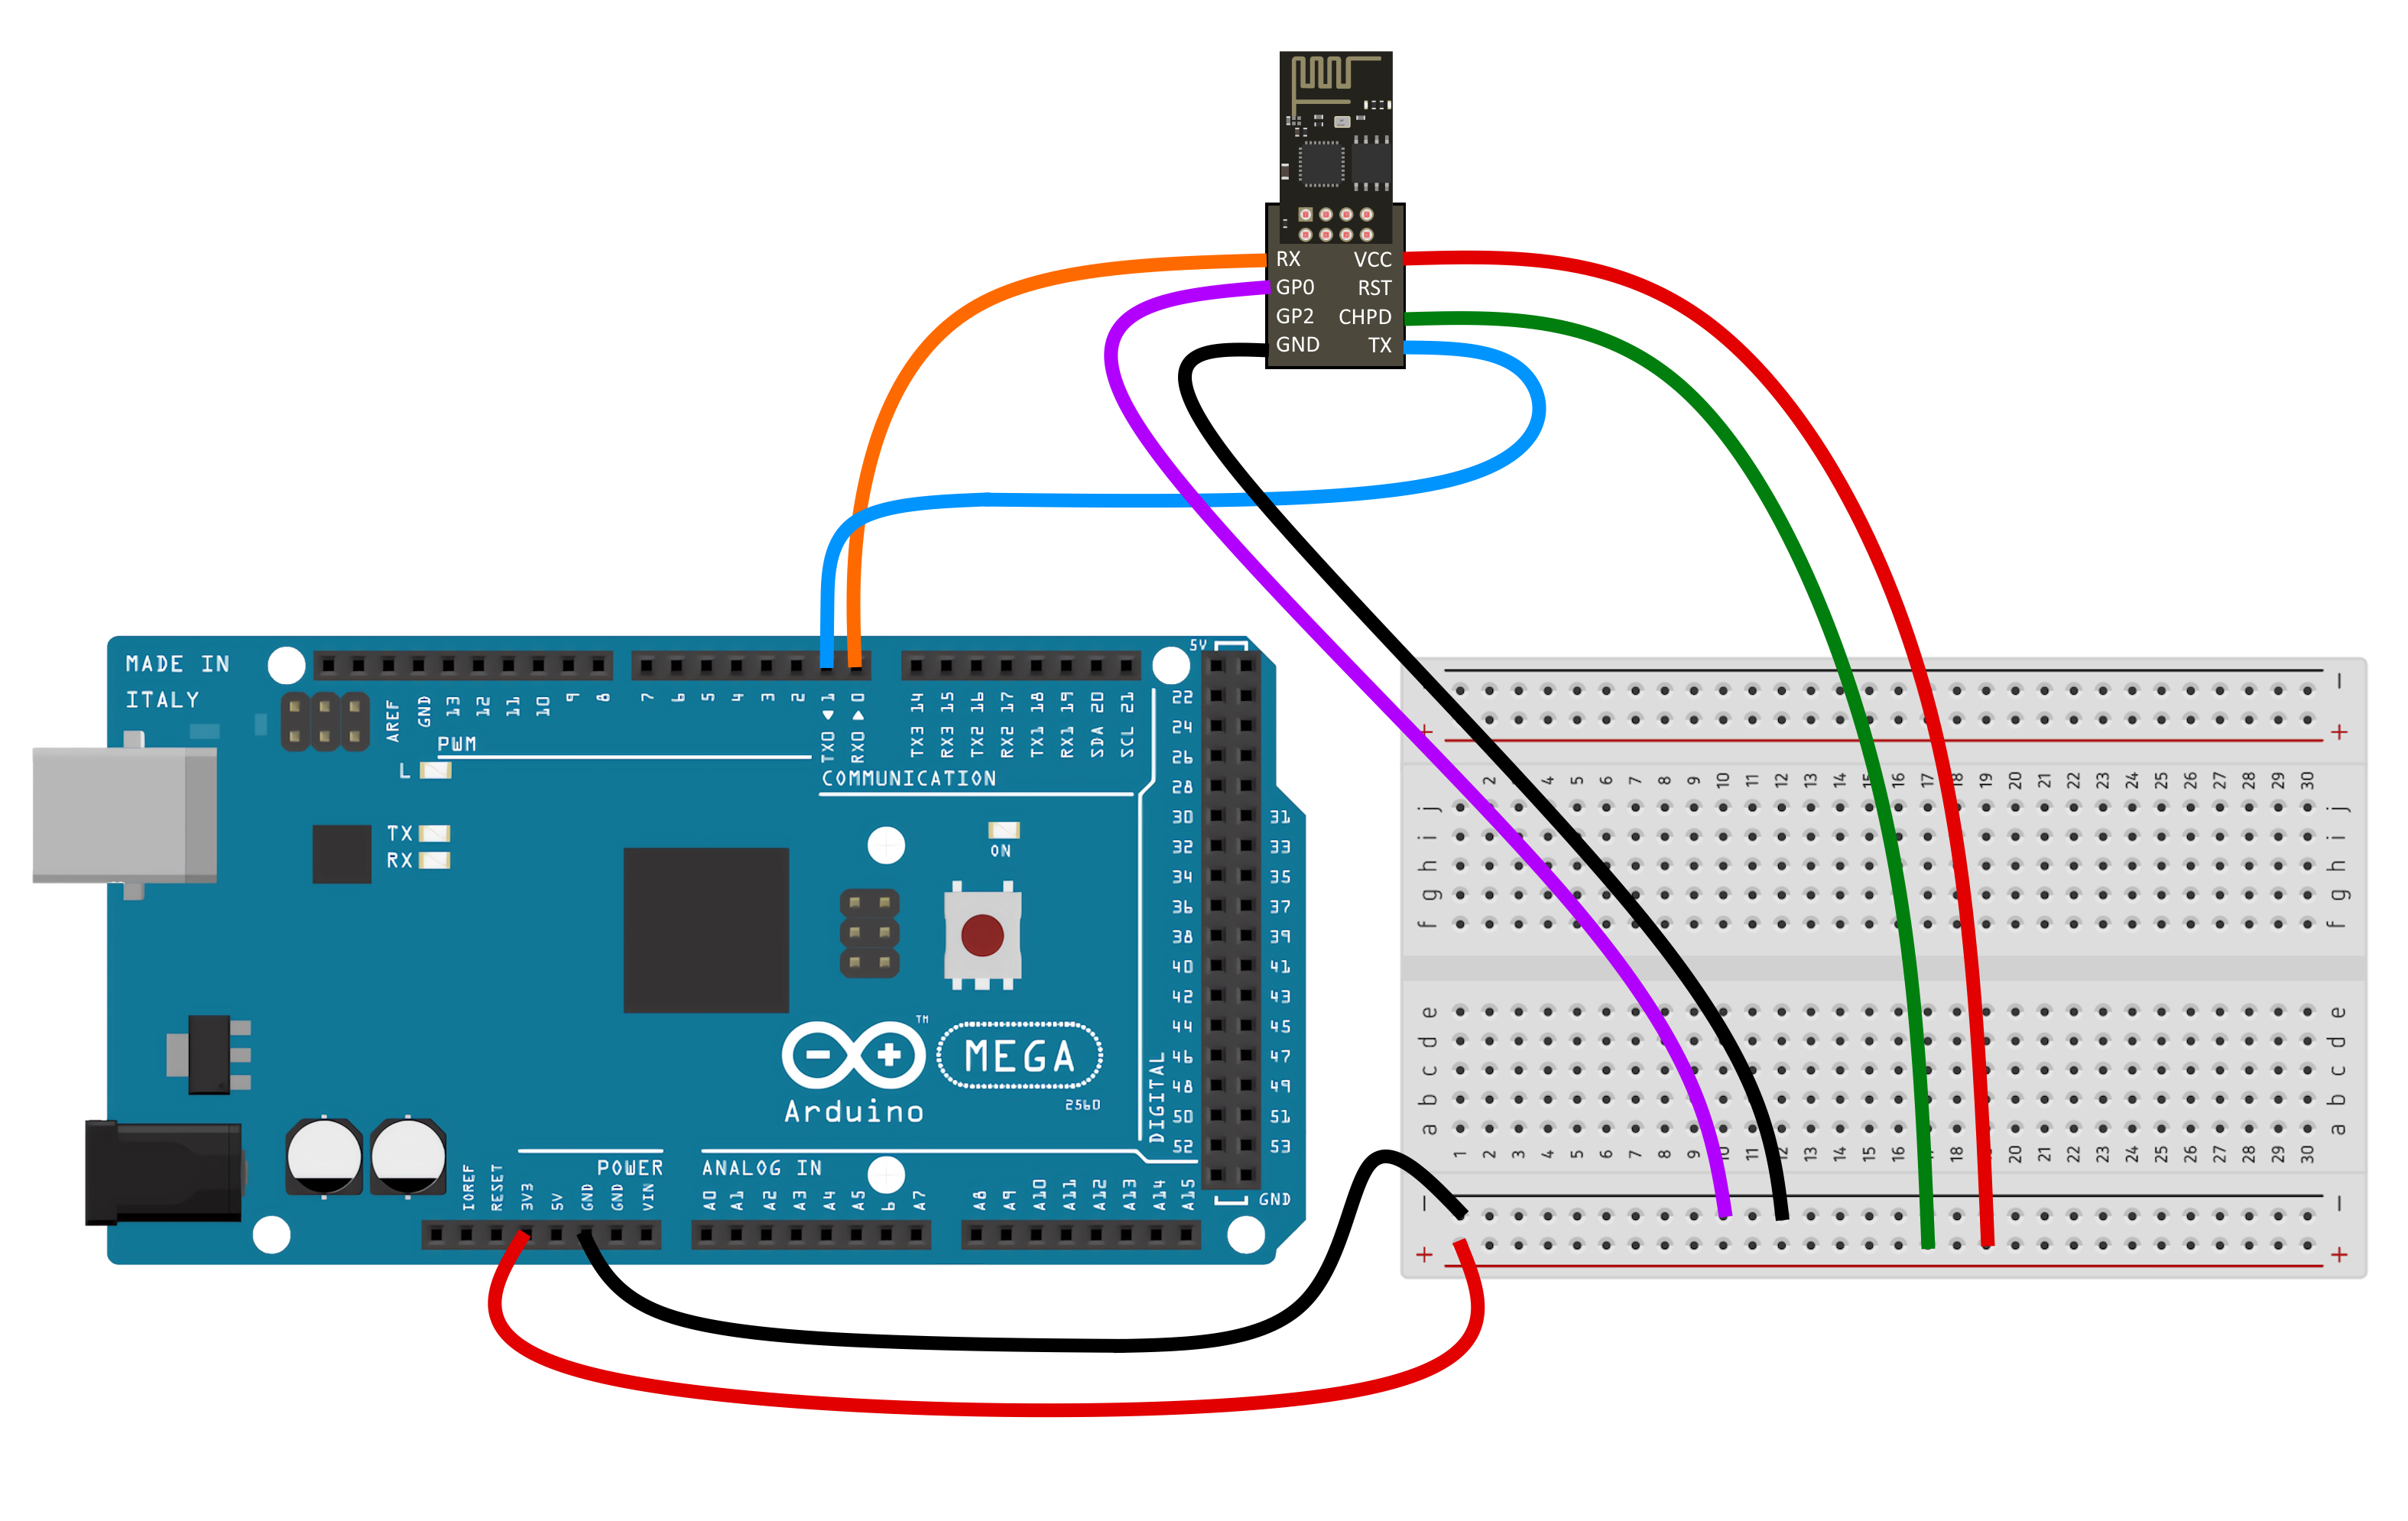
\includegraphics[scale=0.2, center]{esp_circuit.png}
    \caption[Circuit ESP01]{Circuit voor het instellen van de ESP01}
    \label{fig:esp_circuit}
\end{figure}

De juiste flasher software is te vinden in \href{https://drive.google.com/open?id=1tD7IpE4rPMOWyQHP6xzjdRKjJAyeEZPj}{deze} deze Google drive. De juiste firmware is op \href{https://wiki.aprbrother.com/en/Firmware_For_ESP8266.html}{deze} site te vinden, de correcte versie is v0.9.5.2.

Vervolgens kan de juiste firmware worden geüpload door de juiste poort van de Arduino te selecteren en te beginnen met downloaden. Tijdens het downloaden is het belangrijk dat er geen Serial monitors open staan in de Arduino IDE.



\subsection{Instellen van de ESP01}
\label{subsec:instellen}

Nadat de juiste firmware is geïnstalleerd op de ESP01 kan deze worden bereikt met de command-line-interface in de Arduino IDE. Vooraleer er AT-commando's kunnen worden verstuurd moet er een lege applicatie worden geüpload op de Arduino. Zo zal de Arduino ondertussen geen script uitvoeren. Hierna kan de ESP bereikt worden, een kleine test is het commando AT, waarop OK moet worden geantwoord:

\begin{lstlisting}[language=Java,caption={Test of de ESP01 bereikbaar is}]
AT

    OK
\end{lstlisting}

Vervolgens moeten de volgende commando's worden verstuurd:
\begin{lstlisting}[language=Java,caption={ESP01 voorbereiden}]
AT+CIOBAUD=9600 //baud rate veranderen naar 9600

AT+CWMODE=1     //WiFi modus correct instellen

AT+CWJAP="netwerknaam","paswoord"   //ESP01 verbinden met WiFi netwerk

AT+CIPMUX=0     //enkele verbinding inschakelen    
\end{lstlisting}


\section{Visualisatie in Thingspeak via Matlab}
\label{sec:matlab}

\begin{lstlisting}[language=Matlab,caption={Visualisatie in matlab}]
readChannelID = CHANNEL_ID;
readAPIKey = 'READ_API_KEY';

fieldIDs = [1, 2, 3, 4, 5, 6, 7, 8];

% aantal datapunten die worden getoont
numPoints = 10;

% data lezen van Thingspeak
data = thingSpeakRead(readChannelID, 'Fields', fieldIDs, 'NumPoints', numPoints, 'ReadKey', readAPIKey);

% per veld de data selecteren
MQ135_CO2_ppm = data(:, 1);
MQ135_NH4_ppm = data(:, 2);
MQ7_CO_ppm = data(:, 3);
MQ4_CH4_ppm = data(:, 4);
MQ7_H2_ppm = data(:, 5);
MQ4_LPG_ppm = data(:, 6);
Temperature = data(:, 7);
Luchtvochtigheid = data(:, 8);


figure;

subplot(2, 4, 1);
plot(MQ135_CO2_ppm);
title('MQ135 CO2');

subplot(2, 4, 2);
plot(MQ135_NH4_ppm);
title('MQ135 NH4');

subplot(2, 4, 3);
plot(MQ7_CO_ppm);
title('MQ7 CO');

subplot(2, 4, 4);
plot(MQ4_CH4_ppm);
title('MQ4 CH4');

subplot(2, 4, 5);
plot(MQ7_H2_ppm);
title('MQ7 H2');

subplot(2, 4, 6);
plot(MQ4_LPG_ppm);
title('MQ4 LPG');

subplot(2, 4, 7);
plot(Temperature);
title('Temperatuur');

subplot(2, 4, 8);
plot(Luchtvochtigheid);
title('Luchtvochtigheid');

\end{lstlisting}


\section{Instellen van de database}
\label{sec:database}

De databank werd gehost via Apache, dit gebeurde met de hulp van XAMPP. XAMPP is een open source applicatie gemaakt door ApacheFriends. Deze omgeving biedt verschillende diensten aan, zoals de Apache-webserver en MySQL. Via het controle paneel kan Apache worden opgestart waarna deze draait op poort 80. Het is belangrijk dat er in de firewall configuratie van de computer een uitzondering wordt gemaakt voor \verb|C:\xampp\apache\bin\httd.exe|, anders zal Apache worden geblokkeerd.

\begin{figure}[h]
    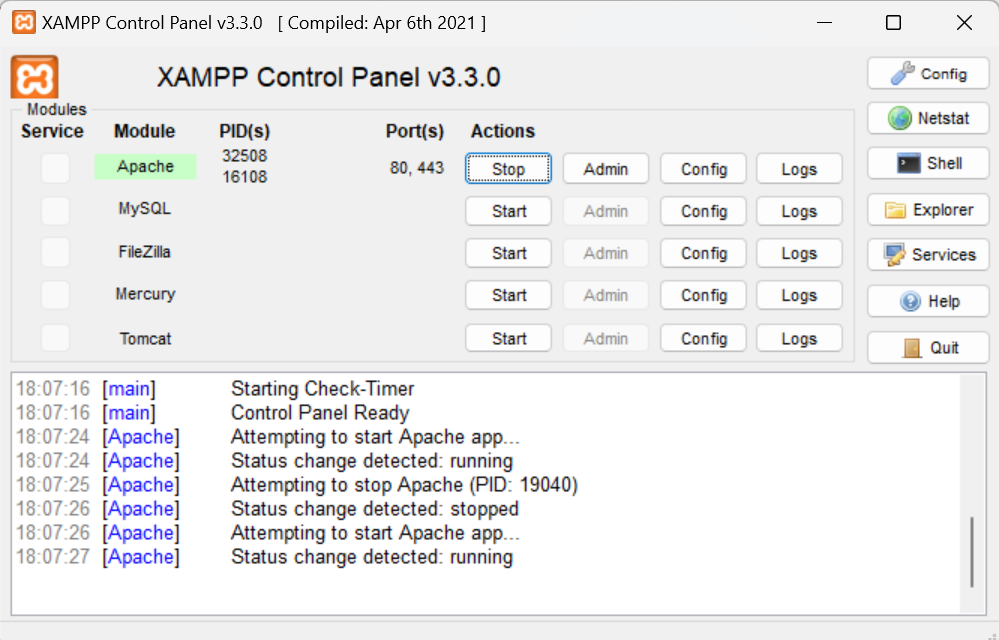
\includegraphics[scale=0.5, center]{XAMPP.png}
    \caption[XAMPP controlepaneel]{Controlepaneel van XAMPP}
    \label{fig:XAMPP}
\end{figure}

Vervolgens moeten de PHP-files worden geschreven, tenslotte moeten deze in de folder \verb|C:\xampp\htdocs| worden gezet staan zodat Apache deze kan vinden.

\section{Finale code}
\label{sec:finale_code}

\subsection{Berekenen van de R\textsubscript{0} waardes}
\label{subsec:script_R0}

\begin{lstlisting}[language=Java,caption={Berekenen en verzenden van de R0 waardes}]
// Kalibratie MQ-4, MQ-135 en MQ-7
// te doen in schone buitenlucht na opwarmperiode van minimaal 5 minuten
#include <SoftwareSerial.h>
#include <stdlib.h>

SoftwareSerial ser(10, 11); // TX, RX
String server = "192.168.1.44"; // ip pc -> zorg dat apache runt

//luchtconstanten uit datasheet
float luchtconstante_MQ4 = 4.4;
float luchtconstante_MQ135 = 3.6;
float luchtconstante_MQ7 = 25.8;

//pinnen vd sensoren 
int MQ4 = A0;
int MQ135 = A1;
int MQ7 = A2;
int mosfet = 9;


float analogeWaarde_MQ4;
float analogeWaarde_MQ135;
float analogeWaarde_MQ7;
float R0_MQ4;
float R0_MQ135;
float R0_MQ7;

void setup() {
    Serial.begin(9600);
    pinMode(MQ7, INPUT);
    pinMode(mosfet, OUTPUT);
    
    ser.begin(9600);
    // reset ESP8266
    ser.println("AT+RST");
}

void loop() {
    
    analogWrite(mosfet, 255); // turn the heater to 5V
    Serial.println("----- 5V voor 60s -----");
    delay(60000); // heat for 60 second
    analogWrite(mosfet, 72); // turn the heater to 1.4V
    Serial.println("----- 1.4V voor 90s -----");
    delay(90000); // wait for 90 seconds | Read values at heater voltage 1.4V
    
    analogeWaarde_MQ4 = analogRead(MQ4);
    analogeWaarde_MQ135 = analogRead(MQ135);
    analogeWaarde_MQ7 = analogRead(MQ7);
    
    R0_MQ4 = R0_berekenen(analogeWaarde_MQ4, luchtconstante_MQ4, 1.0);
    R0_MQ135 = R0_berekenen(analogeWaarde_MQ135, luchtconstante_MQ135, 1.0);
    R0_MQ7 = R0_berekenen(analogeWaarde_MQ7, luchtconstante_MQ7, 10.0);
    
    stuur_naar_DB (R0_MQ4, R0_MQ135, R0_MQ7);
    
    Serial.print("R0 MQ4 = ");
    Serial.println(R0_MQ4);

    Serial.print("R0 MQ135 = ");
    Serial.println(R0_MQ135);

    Serial.print("R0 MQ7 = ");
    Serial.println(R0_MQ7);
}


float R0_berekenen(float analogeWaarde, float luchtconstante, float R_l) {
    float Rs;
    float R0;
    float V_out;
    float V_cc = 5.0;
    float maxAnaloog = 1023.0;
    
    //waarde omzetten naar spanning
    V_out = (analogeWaarde*V_cc)/maxAnaloog;
    
    //Rs berekenen
    Rs = ((V_cc*R_l)/V_out)-R_l;
    
    //R0 berekenen met luchtconstante
    R0 = Rs/luchtconstante;
    
    return R0;
}


void stuur_naar_DB (float R0MQ4, float R0MQ135, float R0MQ7) {
    // TCP connection
    String cmd = "AT+CIPSTART=\"TCP\",\"";
    cmd += server;
    cmd += "\",80";
    Serial.println(cmd);
    ser.println(cmd);
    
    if(ser.find("Error")){
        Serial.println("AT+CIPSTART error");
        return;
    }
    
    String data;
    String uri = "/insertR0.php";
    
    data = "R0_MQ4=" + String(R0_MQ4) + "&R0_MQ135=" + String(R0_MQ135) + "&R0_MQ7=" + String(R0_MQ7);
    
    String postRequest =
    "POST " + uri + " HTTP/1.1\r\n" +
    "Host: " + server + "\r\n" +
    "Connection: keep-alive\r\n"
    "Content-Type: application/x-www-form-urlencoded\r\n" +
    "Content-Length: " + data.length() + "\r\n" +
    "\r\n" + data;
    postRequest += "\r\n\r\n";
    
    // send data length
    cmd = "AT+CIPSEND=";
    cmd += String(postRequest.length());
    ser.println(cmd);
    Serial.println(cmd);
    
    if(ser.find(">")){
        ser.print(postRequest);
        Serial.println(postRequest);
    }
    else{
        ser.println("AT+CIPCLOSE");
        // alert user
        Serial.println("AT+CIPCLOSE");
    }
    
    ser.println("AT+RST");
}
   
\end{lstlisting}

\begin{lstlisting}[language=Java,caption={insertR0.php}]
<?php

$R0_MQ4 = $_POST["R0_MQ4"];
$R0_MQ135 = $_POST["R0_MQ135"];
$R0_MQ7 = $_POST["R0_MQ7"];

$servername = "localhost";
$username = "root";
$password = "root";
$dbname = "db_arduino";

// Create connection
$conn = new mysqli($servername, $username, $password, $dbname);
// Check connection
if ($conn->connect_error) {
    die("Connection failed: " . $conn->connect_error);
}

$sql = "INSERT INTO R0 (R0_MQ4, R0_MQ135, R0_MQ7, gelezen_op) VALUES ($R0_MQ4, $R0_MQ135, $R0_MQ7, NOW())";
if ($conn->query($sql) === TRUE) {
    echo "New record created successfully";
} else {
    echo "Error: " . $sql . " => " . $conn->error;
}

$conn->close();

?>

\end{lstlisting}

\subsection{MQ sensoren naar Thingspeak}
\label{subsec:script_thingspeak}

\begin{lstlisting}[language=Java,caption={MQ sensoren naar Thingspeak}]
//           //
// Libraries //
//           //
#include <SoftwareSerial.h>
#include <stdlib.h>
#include <dht.h>
dht DHT;

//            //
// Variabelen //
//            //
String apiKey = "WRITE_API_KEY";

//R0 berekent met kalibratie script
float R0_MQ4 = 4.88;
float R0_MQ135 = 9.59;
float R0_MQ7 = 16.33;

float Rs_MQ4;
float Rs_MQ135;
float Rs_MQ7;

//pinnen vd sensoren 
int MQ4 = A0;
int MQ135 = A1;
int MQ7 = A2;
int mosfet = 9;
#define DHT22 2

float analogeWaarde_MQ4;
float analogeWaarde_MQ135;
float analogeWaarde_MQ7;

float MQ4_LPG_ppm;
float MQ4_CH4_ppm;
float MQ135_NH4_ppm;
float MQ135_CO2_ppm;
float MQ7_CO_ppm;
float MQ7_H2_ppm;

//waarden van grafieken
float MQ4_LPG[4] = {224.99, 2.47, 9184.24, 0.75};
float MQ4_CH4[4] = {222.75, 1.68, 9184.24, 0.45};
float MQ135_NH4[4] = {10.61, 2.49, 190.20, 0.77};
float MQ135_CO2[4] = {10.72, 2.78, 191.15, 1.35};
float MQ7_CO[4] = {53.60, 1.51, 3552.21, 0.09};
float MQ7_H2[4] = {54.85, 1.19, 3525.08, 0.05};

float vochtigheid;
float temperatuur;


SoftwareSerial ESP(10, 11); // TX, RX

//       //
// Setup //
//       //
void setup() {
    Serial.begin(9600);
    ESP.begin(9600);
    pinMode(MQ7, INPUT);
    pinMode(mosfet, OUTPUT);
    
    // reset ESP
    ESP.println("AT+RST");
}


//           //
// Main loop //
//           //
void loop() {
    // MQ7 hoog (voor 60 sec)
    analogWrite(mosfet, 255); //5V naar MQ7
    Serial.println("5V naar MQ7");
    // 4 * MQ (15 sec) naar Thingspeak
    delay(15000);
    for (int i = 0; i < 3; i++) {
        sensoren_berekenen_en_sturen(false); //zonder MQ7
        delay(15000);
    }
    // MQ7 laag (voor 90 sec)
    analogWrite(mosfet, 72); //1.4V naar MQ7
    Serial.println("5V naar MQ7");
    // 6 * MQ (15 sec) naar Thingspeak
    for (int i = 0; i < 6; i++) {
        sensoren_berekenen_en_sturen(false); //zonder MQ7
        delay(15000);
    }
    sensoren_berekenen_en_sturen(true); //MQ7 cyclus is klaar dus met mq7
}

void sensoren_berekenen_en_sturen(bool MQ7) {
    String waarde_MQ4;
    String waarde_MQ135;
    String waarde_MQ7;
    String waarde_DHT;
    int x = DHT.read22(DHT22);
    vochtigheid = DHT.humidity;
    temperatuur = DHT.temperature;
    
    analogeWaarde_MQ4 = analogRead(MQ4);
    analogeWaarde_MQ135 = analogRead(MQ135);
    
    Rs_MQ4 = Rs_berekenen(analogeWaarde_MQ4, 1.0); //Rl van 1
    Rs_MQ135 = Rs_berekenen(analogeWaarde_MQ135, 1.0); //Rl van 1
    
    MQ4_LPG_ppm = ppm_berekenen(R0_MQ4, Rs_MQ4, MQ4_LPG, 4, temperatuur, vochtigheid);
    MQ4_CH4_ppm = ppm_berekenen(R0_MQ4, Rs_MQ4, MQ4_CH4, 4, temperatuur, vochtigheid);
    MQ135_NH4_ppm = ppm_berekenen(R0_MQ135, Rs_MQ135, MQ135_NH4, 135, temperatuur, vochtigheid);
    MQ135_CO2_ppm = ppm_berekenen(R0_MQ135, Rs_MQ135, MQ135_CO2, 135, temperatuur, vochtigheid);
    
    waarde_MQ4 = "field4="+String(MQ4_CH4_ppm)+"&field6="+String(MQ4_LPG_ppm);
    waarde_MQ135 = "field1="+String(MQ135_CO2_ppm)+"&field2="+String(MQ135_NH4_ppm);
    waarde_DHT = "field7="+String(temperatuur)+"&field8="+String(vochtigheid);
    
    if (MQ7) {
        analogeWaarde_MQ7 = analogRead(MQ7);
        Rs_MQ7 = Rs_berekenen(analogeWaarde_MQ7, 10.0); //Rl van 10
        MQ7_CO_ppm = ppm_berekenen(R0_MQ7, Rs_MQ7, MQ7_CO), 7, temperatuur, vochtigheid;
        MQ7_H2_ppm = ppm_berekenen(R0_MQ7, Rs_MQ7, MQ7_H2, 7, temperatuur, vochtigheid);
        waarde_MQ7 = "field3="+String(MQ7_CO_ppm)+"&field5="+String(MQ7_H2_ppm);
        
        thingspeak(waarde_MQ4+"&"+waarde_MQ135+"&"+waarde_MQ7+"&"+waarde_DHT);
    } else {
        thingspeak(waarde_MQ4+"&"+waarde_MQ135+"&"+waarde_DHT);
    }
    
}


void thingspeak(String waarde) {
    // TCP connection
    String cmd = "AT+CIPSTART=\"TCP\",\"";
    cmd += "184.106.153.149"; // api.thingspeak.com
    cmd += "\",80";
    //Serial.println(cmd);
    ESP.println(cmd);
    
    if(ESP.find("ERROR")){
        Serial.println("AT+CIPSTART error");
        return;
    }
    
    // prepare GET string
    String getStr = "GET /update?api_key=";
    getStr += apiKey;
    getStr +="&";
    getStr += waarde;
    getStr += "\r\n\r\n";
    
    // send data length
    cmd = "AT+CIPSEND=";
    cmd += String(getStr.length());
    ESP.println(cmd);
    Serial.println(cmd);
    
    if(ESP.find(">")){
        ESP.print(getStr);
        Serial.println(getStr);
    }
    else{
        ESP.println("AT+CIPCLOSE");
        // alert user
        Serial.println("AT+CIPCLOSE");
    }
    
    ESP.println("AT+RST");
}

float Rs_berekenen(float analogeWaarde, float R_l) {
    float Rs;
    float V_out;
    float V_cc = 5.0;
    float maxAnaloog = 1023.0;
    
    //waarde omzetten naar spanning
    V_out = (analogeWaarde*V_cc)/maxAnaloog;
    
    //Rs berekenen
    Rs = ((V_cc*R_l)/V_out)-R_l;
    
    return Rs;
}

float ppm_berekenen(float R0, float Rs, float waarden[4], int sensortype, float temperatuur, float vochtigheid) {
    float b;
    float m;
    float ppm;
    
    m = (log10(waarden[3])-log10(waarden[1]))/(log10(waarden[2])-log10(waarden[0]));
    b = log10(waarden[1]) - m*log10(waarden[0]);
    float corr_factor = bereken_correctiefactor(sensortype, temperatuur, vochtigheid);
    
    ppm = pow((Rs*corr_factor/(R0*pow(10, b))),(1/m));
    
    return ppm;
}

float bereken_correctiefactor(int sensor, float temp, float hum) {
    float y_33;
    float y_85;
    if (temp > 20) {
        switch (sensor) {
            case 4:
            y_33 = -0.00295586181504405 * temp + 1.0533607677395043;
            y_85 = -0.004342063209608854 * temp + 0.937042646891705;
            break;
            case 7:
            y_33 = -0.004424792057792776 * temp + 1.0851404282394788;
            y_85 = -0.0039878849252431 * temp + 0.9353690615195733;
            break;
            case 135:
            y_33 = -0.002329525704310693 * temp + 1.026785488456616;
            y_85 = -0.002731083213397648 * temp + 0.9528596643559701;
            break;
            default:
            Serial.println("Foute sensor");
            break;
        }
    } else {
        switch (sensor) {
            case 4:
            y_33 = 0.00021598016836642446 * pow(temp,2) - 0.011780605617435404 * temp + 1.1489572784939854;
            y_85 = 0.00011618781246091718 * pow(temp,2) - 0.009401474805251435 * temp + 0.9921017705779126;
            break;
            case 7:
            y_33 = 0.0004604255602040132 * pow(temp,2) - 0.019452899554979888 * temp + 1.2135189729083746;
            y_85 = 0.00020619142958797082 * pow(temp,2) - 0.01249218944803551 * temp + 1.0274335776434782;
            break;
            case 135:
            y_33 = 0.00046307428153304244 * pow(temp,2) - 0.02906738438091286 * temp + 1.3784941304658396;
            y_85 = 0.0004117696144765908 * pow(temp,2) - 0.025339923585248027 * temp + 1.245958990497358;
            break;
            default:
            Serial.println("Foute sensor");
            break;
        }
    }
    return y_33 + ((y_85-y_33)/(85-33))*(hum-33);
}
        
\end{lstlisting}

\begin{lstlisting}[language=Java,caption={insertDB.php}]
<?php

$MQ4_CO_ppm = $_POST["MQ4_CO_ppm"];
$MQ4_alcohol_ppm = $_POST["MQ4_alcohol_ppm"];
$MQ4_rook_ppm = $_POST["MQ4_rook_ppm"];
$MQ4_H2_ppm = $_POST["MQ4_H2_ppm"];
$MQ4_LPG_ppm = $_POST["MQ4_LPG_ppm"];
$MQ4_CH4_ppm = $_POST["MQ4_CH4_ppm"];

$MQ135_CO_ppm = $_POST["MQ135_CO_ppm"];
$MQ135_NH4_ppm = $_POST["MQ135_NH4_ppm"];
$MQ135_CO2_ppm = $_POST["MQ135_CO2_ppm"];
$MQ135_alcohol_ppm = $_POST["MQ135_alcohol_ppm"];
$MQ135_tolueen_ppm = $_POST["MQ135_tolueen_ppm"];
$MQ135_aceton_ppm = $_POST["MQ135_aceton_ppm"];

$MQ7_alcohol_ppm = $_POST["MQ7_alcohol_ppm"];
$MQ7_CH4_ppm = $_POST["MQ7_CH4_ppm"];
$MQ7_LPG_ppm = $_POST["MQ7_LPG_ppm"];
$MQ7_CO_ppm = $_POST["MQ7_CO_ppm"];
$MQ7_H2_ppm = $_POST["MQ7_H2_ppm"];

$vochtigheid = $_POST["hum"];
$temperatuur = $_POST["temp"];

$servername = "localhost";
$username = "root";
$password = "root";
$dbname = "db_arduino";

// Create connection
$conn = new mysqli($servername, $username, $password, $dbname);
// Check connection
if ($conn->connect_error) {
    die("Connection failed: " . $conn->connect_error);
}

$sql = "INSERT INTO MQ4 (CO, alcohol, rook, H2, LPG, CH4, gelezen_op) VALUES ($MQ4_CO_ppm, $MQ4_alcohol_ppm, $MQ4_rook_ppm, $MQ4_H2_ppm, $MQ4_LPG_ppm, $MQ4_CH4_ppm, NOW())";
if ($conn->query($sql) === TRUE) {
    echo "New record created successfully";
} else {
    echo "Error: " . $sql . " => " . $conn->error;
}
$sql = "INSERT INTO MQ135 (CO, NH4, CO2, alcohol, tolueen, aceton, gelezen_op) VALUES ($MQ135_CO_ppm, $MQ135_NH4_ppm, $MQ135_CO2_ppm, $MQ135_alcohol_ppm, $MQ135_tolueen_ppm, $MQ135_aceton_ppm, NOW())";
if ($conn->query($sql) === TRUE) {
    echo "New record created successfully";
} else {
    echo "Error: " . $sql . " => " . $conn->error;
}
$sql = "INSERT INTO MQ7 (alcohol, CH4, LPG, CO, H2, gelezen_op) VALUES ($MQ7_alcohol_ppm, $MQ7_CH4_ppm, $MQ7_LPG_ppm, $MQ7_CO_ppm, $MQ7_H2_ppm, NOW())";
if ($conn->query($sql) === TRUE) {
    echo "New record created successfully";
} else {
    echo "Error: " . $sql . " => " . $conn->error;
}
$sql = "INSERT INTO DHT22 (vochtigheid, temperatuur, gelezen_op) VALUES ($vochtigheid, $temperatuur, NOW())";
if ($conn->query($sql) === TRUE) {
    echo "New record created successfully";
} else {
    echo "Error: " . $sql . " => " . $conn->error;
}

$conn->close();

?>

\end{lstlisting}


\subsection{MQ sensoren naar de databank}
\label{subsec:script_db}

\begin{lstlisting}[language=Java,caption={MQ sensoren naar de databank}]
//           //
// Libraries //
//           //
#include <SoftwareSerial.h>
#include <stdlib.h>
#include <dht.h>
dht DHT;

//            //
// Variabelen //
//            //
String server = "192.168.1.44"; // ip pc -> zorg dat apache runt

//R0 berekent met kalibratie script
float R0_MQ4 = 4.88;
float R0_MQ135 = 9.59;
float R0_MQ7 = 16.33;

float Rs_MQ4;
float Rs_MQ135;
float Rs_MQ7;

//pinnen vd sensoren 
int MQ4 = A0;
int MQ135 = A1;
int MQ7 = A2;
int mosfet = 9;
#define DHT22 2

float analogeWaarde_MQ4;
float analogeWaarde_MQ135;
float analogeWaarde_MQ7;

float vochtigheid;
float temperatuur;

float MQ4_CO_ppm;
float MQ4_alcohol_ppm;
float MQ4_rook_ppm;
float MQ4_H2_ppm;
float MQ4_LPG_ppm;
float MQ4_CH4_ppm;
float MQ135_CO_ppm;
float MQ135_NH4_ppm;
float MQ135_CO2_ppm;
float MQ135_alcohol_ppm;
float MQ135_tolueen_ppm;
float MQ135_aceton_ppm;
float MQ7_alcohol_ppm;
float MQ7_CH4_ppm;
float MQ7_LPG_ppm;
float MQ7_CO_ppm;
float MQ7_H2_ppm;

//waarden van grafieken
float MQ4_CO[4] = {230.69, 4.23, 9369.99, 3.51};
float MQ4_alcohol[4] = {218.33, 4.00, 9092.75, 3.08};
float MQ4_rook[4] = {223.87, 3.89, 9138.38, 2.57};
float MQ4_H2[4] = {222.75, 3.71, 9276.65, 1.92};
float MQ4_LPG[4] = {224.99, 2.47, 9184.24, 0.75};
float MQ4_CH4[4] = {222.75, 1.68, 9184.24, 0.45};

float MQ135_CO2[4] = {10.72, 2.78, 191.15, 1.35};
float MQ135_NH4[4] = {10.61, 2.49, 190.20, 0.77};
float MQ135_CO[4] = {10.72, 2.24, 188.31, 0.81};
float MQ135_alcohol[4] = {10.51, 1.86, 189.25, 0.74};
float MQ135_tolueen[4] = {10.45, 1.52, 188.31, 0.65};
float MQ135_aceton[4] = {10.72, 1.39, 189.25, 0.59};

float MQ7_alcohol[4] = {56.12, 15.88, 3525.08, 12.23};
float MQ7_CH4[4] = {56.55, 13.70, 3634.86, 9.20};
float MQ7_LPG[4] = {53.19, 8.90, 3498.16, 5.10};
float MQ7_CO[4] = {53.60, 1.51, 3552.21, 0.09};
float MQ7_H2[4] = {54.85, 1.19, 3525.08, 0.05};



SoftwareSerial ESP(10, 11); // TX, RX

//       //
// Setup //
//       //
void setup() {
    Serial.begin(9600);
    ESP.begin(9600);
    pinMode(MQ7, INPUT);
    pinMode(mosfet, OUTPUT);
    
    // reset ESP
    ESP.println("AT+RST");
}


//           //
// Main loop //
//           //
void loop() {
    // MQ7 hoog (voor 60 sec)
    analogWrite(mosfet, 255); //5V naar MQ7
    Serial.println("5V naar MQ7");
    delay(60000);
    // MQ7 laag (voor 90 sec)
    analogWrite(mosfet, 72); //1.4V naar MQ7
    Serial.println("1.4V naar MQ7");
    delay(90000);
    
    sensoren_berekenen_en_sturen();
}

void sensoren_berekenen_en_sturen() {
    String waarde_MQ4;
    String waarde_MQ135;
    String waarde_MQ7;
    String waarde_DHT;
    
    int x = DHT.read22(DHT22);
    vochtigheid = DHT.humidity;
    temperatuur = DHT.temperature;
    
    analogeWaarde_MQ4 = analogRead(MQ4);
    analogeWaarde_MQ135 = analogRead(MQ135);
    analogeWaarde_MQ7 = analogRead(MQ7);
    
    Rs_MQ4 = Rs_berekenen(analogeWaarde_MQ4, 1.0); //Rl van 1
    Rs_MQ135 = Rs_berekenen(analogeWaarde_MQ135, 1.0); //Rl van 1
    Rs_MQ7 = Rs_berekenen(analogeWaarde_MQ7, 10.0); //Rl van 10
    
    MQ4_CO_ppm = ppm_berekenen(R0_MQ4, Rs_MQ4, MQ4_CO, 4, temperatuur, vochtigheid);
    MQ4_alcohol_ppm = ppm_berekenen(R0_MQ4, Rs_MQ4, MQ4_alcohol, 4, temperatuur, vochtigheid);
    MQ4_rook_ppm = ppm_berekenen(R0_MQ4, Rs_MQ4, MQ4_rook, 4, temperatuur, vochtigheid);
    MQ4_H2_ppm = ppm_berekenen(R0_MQ4, Rs_MQ4, MQ4_H2, 4, temperatuur, vochtigheid);
    MQ4_LPG_ppm = ppm_berekenen(R0_MQ4, Rs_MQ4, MQ4_LPG, 4, temperatuur, vochtigheid);
    MQ4_CH4_ppm = ppm_berekenen(R0_MQ4, Rs_MQ4, MQ4_CH4, 4, temperatuur, vochtigheid);
    MQ135_CO_ppm = ppm_berekenen(R0_MQ135, Rs_MQ135, MQ135_CO, 135, temperatuur, vochtigheid);
    MQ135_NH4_ppm = ppm_berekenen(R0_MQ135, Rs_MQ135, MQ135_NH4, 135, temperatuur, vochtigheidv);
    MQ135_CO2_ppm = ppm_berekenen(R0_MQ135, Rs_MQ135, MQ135_CO2, 135, temperatuur, vochtigheid);
    MQ135_alcohol_ppm = ppm_berekenen(R0_MQ135, Rs_MQ135, MQ135_alcohol, 135, temperatuur, vochtigheid);
    MQ135_tolueen_ppm = ppm_berekenen(R0_MQ135, Rs_MQ135, MQ135_tolueen, 135, temperatuur, vochtigheid);
    MQ135_aceton_ppm = ppm_berekenen(R0_MQ135, Rs_MQ135, MQ135_aceton, 135, temperatuur, vochtigheid);
    MQ7_alcohol_ppm = ppm_berekenen(R0_MQ7, Rs_MQ7, MQ7_alcohol, 7, temperatuur, vochtigheid);
    MQ7_CH4_ppm = ppm_berekenen(R0_MQ7, Rs_MQ7, MQ7_CH4, 7, temperatuur, vochtigheid);
    MQ7_LPG_ppm = ppm_berekenen(R0_MQ7, Rs_MQ7, MQ7_LPG, 7, temperatuur, vochtigheid);
    MQ7_CO_ppm = ppm_berekenen(R0_MQ7, Rs_MQ7, MQ7_CO, 7, temperatuur, vochtigheid);
    MQ7_H2_ppm = ppm_berekenen(R0_MQ7, Rs_MQ7, MQ7_H2, 7, temperatuur, vochtigheid);
    
    waarde_MQ4 = "MQ4_CO_ppm="+String(MQ4_CO_ppm)+"&MQ4_alcohol_ppm="+String(MQ4_alcohol_ppm)+"&MQ4_rook_ppm="+String(MQ4_rook_ppm)+"&MQ4_H2_ppm="+String(MQ4_H2_ppm)+"&MQ4_LPG_ppm="+String(MQ4_LPG_ppm)+"&MQ4_CH4_ppm="+String(MQ4_CH4_ppm);
    waarde_MQ135 ="MQ135_CO_ppm="+String(MQ135_CO_ppm)+"&MQ135_NH4_ppm="+String(MQ135_NH4_ppm)+"&MQ135_CO2_ppm="+String(MQ135_CO2_ppm)+"&MQ135_alcohol_ppm="+String(MQ135_alcohol_ppm)+"&MQ135_tolueen_ppm="+String(MQ135_tolueen_ppm)+"&MQ135_aceton_ppm="+String(MQ135_aceton_ppm);
    waarde_MQ7 = "MQ7_alcohol_ppm="+String(MQ7_alcohol_ppm)+"&MQ7_CH4_ppm="+String(MQ7_CH4_ppm)+"&MQ7_LPG_ppm="+String(MQ7_LPG_ppm)+"&MQ7_CO_ppm="+String(MQ7_CO_ppm)+"&MQ7_H2_ppm="+String(MQ7_H2_ppm);
    waarde_DHT = "temp="+String(temperatuur)+"&hum="+String(vochtigheid);
    
    stuur_naar_DB(waarde_MQ4+"&"+waarde_MQ135+"&"+waarde_MQ7+"&"+waarde_DHT);  
}



void stuur_naar_DB (String waarde) {
    String php = "insertDB.php";
    // TCP connection
    String cmd = "AT+CIPSTART=\"TCP\",\"";
    cmd += server;
    cmd += "\",80";
    Serial.println(cmd);
    ESP.println(cmd);
    
    if(ESP.find("Error")){
        Serial.println("AT+CIPSTART error");
        return;
    }
    
    String postRequest =
    "POST /" + php + " HTTP/1.1\r\n" +
    "Host: " + server + "\r\n" +
    "Connection: keep-alive\r\n"
    "Content-Type: application/x-www-form-urlencoded\r\n" +
    "Content-Length: " + waarde.length() + "\r\n" +
    "\r\n" + waarde;
    postRequest += "\r\n\r\n";
    
    // send data length
    cmd = "AT+CIPSEND=";
    cmd += String(postRequest.length());
    ESP.println(cmd);
    Serial.println(cmd);
    
    if(ESP.find(">")){
        ESP.print(postRequest);
        Serial.println(postRequest);
    }
    else{
        ESP.println("AT+CIPCLOSE");
        // alert user
        Serial.println("AT+CIPCLOSE");
    }
    
    ESP.println("AT+RST");
}


float Rs_berekenen(float analogeWaarde, float R_l) {
    float Rs;
    float V_out;
    float V_cc = 5.0;
    float maxAnaloog = 1023.0;
    
    //waarde omzetten naar spanning
    V_out = (analogeWaarde*V_cc)/maxAnaloog;
    
    //Rs berekenen
    Rs = ((V_cc*R_l)/V_out)-R_l;
    
    return Rs;
}

float ppm_berekenen(float R0, float Rs, float waarden[4], int sensortype, float temperatuur, float vochtigheid) {
    float b;
    float m;
    float ppm;
    
    m = (log10(waarden[3])-log10(waarden[1]))/(log10(waarden[2])-log10(waarden[0]));
    b = log10(waarden[1]) - m*log10(waarden[0]);
    float corr_factor = bereken_correctiefactor(sensortype, temperatuur, vochtigheid);
    
    ppm = pow((Rs*corr_factor/(R0*pow(10, b))),(1/m));
    
    return ppm;
}

float bereken_correctiefactor(int sensor, float temp, float hum) {
    float y_33;
    float y_85;
    if (temp > 20) {
        switch (sensor) {
            case 4:
            y_33 = -0.00295586181504405 * temp + 1.0533607677395043;
            y_85 = -0.004342063209608854 * temp + 0.937042646891705;
            break;
            case 7:
            y_33 = -0.004424792057792776 * temp + 1.0851404282394788;
            y_85 = -0.0039878849252431 * temp + 0.9353690615195733;
            break;
            case 135:
            y_33 = -0.002329525704310693 * temp + 1.026785488456616;
            y_85 = -0.002731083213397648 * temp + 0.9528596643559701;
            break;
            default:
            Serial.println("Foute sensor");
            break;
        }
    } else {
        switch (sensor) {
            case 4:
            y_33 = 0.00021598016836642446 * pow(temp,2) - 0.011780605617435404 * temp + 1.1489572784939854;
            y_85 = 0.00011618781246091718 * pow(temp,2) - 0.009401474805251435 * temp + 0.9921017705779126;
            break;
            case 7:
            y_33 = 0.0004604255602040132 * pow(temp,2) - 0.019452899554979888 * temp + 1.2135189729083746;
            y_85 = 0.00020619142958797082 * pow(temp,2) - 0.01249218944803551 * temp + 1.0274335776434782;
            break;
            case 135:
            y_33 = 0.00046307428153304244 * pow(temp,2) - 0.02906738438091286 * temp + 1.3784941304658396;
            y_85 = 0.0004117696144765908 * pow(temp,2) - 0.025339923585248027 * temp + 1.245958990497358;
            break;
            default:
            Serial.println("Foute sensor");
            break;
        }
    }
    return y_33 + ((y_85-y_33)/(85-33))*(hum-33);
}

\end{lstlisting}


\subsection{Warmte-koelcyclus MQ7}
\label{subsec:script_mq7}

\begin{lstlisting}[language=Java,caption={Warmte-koelcyclus van de MQ7}]
//           //
// Libraries //
//           //
#include <dht.h>
dht DHT;

//            //
// Variabelen //
//            //
//pinnen vd sensoren 
int MQ7 = A2;
int mosfet = 9;
#define DHT22 2

float analogeWaarde_MQ7;

float vochtigheid;
float temperatuur;

//       //
// Setup //
//       //
void setup() {
    Serial.begin(9600);
    pinMode(MQ7, INPUT);
    pinMode(mosfet, OUTPUT);
}


//           //
// Main loop //
//           //
void loop() {
    // MQ7 hoog (voor 60 sec)
    analogWrite(mosfet, 255); //5V naar MQ7
    for (int j = 0; j < 30; j++) {
        DHT_en_MQ7_sturen(5.0);
        delay(2000);
    }
    // MQ7 laag (voor 90 sec)
    analogWrite(mosfet, 72); //1.4V naar MQ7
    for (int j = 0; j < 45; j++) {
        DHT_en_MQ7_sturen(1.4);
        delay(2000);
    }
}

void DHT_en_MQ7_sturen(float voltage) {
    String waarde;
    analogeWaarde_MQ7 = analogRead(MQ7);
    int x = DHT.read22(DHT22);
    vochtigheid = DHT.humidity;
    temperatuur = DHT.temperature;
    
    Serial.println("INSERT INTO MQ7_analoog (voltage, analoge_waarde) VALUES ("+String(voltage)+", "+String(analogeWaarde_MQ7)+");");
    Serial.println("INSERT INTO DHT22 (vochtigheid, temperatuur) VALUES ("+String(vochtigheid)+", "+String(temperatuur)+");");
}

\end{lstlisting}










%%---------- Backmatter, referentielijst ---------------------------------------

\backmatter{}

\setlength\bibitemsep{2pt} %% Add Some space between the bibliograpy entries
\nocite{*}
\printbibliography[heading=bibintoc]

\end{document}
